\documentclass[12pt]{book}
\usepackage{fontspec} % Use fontspec for font management
\usepackage{polyglossia} % For multilingual support
\setmainlanguage{english}
\setotherlanguage{greek}

% Set a font that supports both English and Greek
\setmainfont{Times New Roman} % Example font, replace with any suitable font installed on your system

% Define \tightlist to handle Pandoc's list conversion
\providecommand{\tightlist}{%
  \setlength{\itemsep}{0pt}\setlength{\parskip}{0pt}}

% Include necessary packages for tables and hyperlinks
\usepackage{amssymb} % Provides additional symbols
\usepackage{longtable} % For long tables
\usepackage{booktabs} % For better table rules
\usepackage{hyperref} % For hyperlinks

\title{Historical Jesus as the Son of God: Glory to the Newborn King}
\author{MV Data sp. z o.o.}
\date{2025}

\begin{document}

\maketitle

\tableofcontents

\chapter*{Preface}
\begin{itemize}
\item
  Historical Jesus as the Son of God: Glory to the Newborn King
\end{itemize}

\section{Preface}\label{par:preface}

Few figures in history have generated as many competing portraits as Jesus of Nazareth.
Few movements have been as dissected, debated, and reimagined as early Christianity.
Across centuries of inquiry, scholars and theologians have offered radically different answers to the question: Who was Jesus, and what was the origin of the movement that carried his name?

Some say he was the divine Son of God, performing miracles and rising from the dead.
Others see him as an apocalyptic prophet, a rabbi, a revolutionary zealot, a Cynic philosopher, a mystic, a Jewish messiah, a prophet of Allah, a purely mythical creation, or even an actual supernatural being.
Every one of these portraits points to real evidence, and every one has shaped entire schools of thought.

And yet — none has prevailed.
Each model explains something powerfully, but collapses when tested against the evidence as a whole.
This is why the “quest for the historical Jesus” has been renewed again and again for over two centuries: not because the question is trivial, but because no proposed solution has yet fit all the data.

The paradox is sharp: Jesus and early Christianity are among the best-documented figures and movements of antiquity, yet no reconstruction has managed to hold the evidence together without breaking at key points.

This book takes a different approach.
Its foundation is the use of artificial intelligence to synthesize an archive larger than any single human could absorb: two millennia of historical writing, theological speculation, textual criticism, archaeology, and cultural commentary.
Each generation of scholars left insights, but also blind spots.
AI allows us to read them all at once — to uncover patterns, to highlight contradictions, and to recover questions that have been hiding in plain sight.

With the AI-assisted synthesis we apply to it the scientific method.
Every hypothesis is tested against the entire body of data.
The moment a contradiction appears, the hypothesis must be revised or abandoned.
Only the model that survives these collisions — that accounts for more evidence and leaves fewer anomalies than all rivals — deserves to stand.

This is not a shortcut.
It is the opposite: the cumulative labor of countless scholars, disciplined by the logic of scientific testing, now brought into one field of vision.
Secondly, the AI can help us remove the biases that inevitably come from continued reliance on past scholarship and authority that often becomes so ingrained in anyone studying the subject in depth.
There have been countless brilliant points and insights that have been dismissed or ignored because they did not fit the prevailing narrative.
Devoted christians would not read a book openly criticizing religion.
Secular scholars would not listen to valid points made by religious scholars.
And scientific scholars would not consider points made by theories of Ancient Aliens.
And although the final analysis may not agree with a majority of viewpoints of many particular scholars, we find countless deeply insightful observations and fantastic arguments from all groups whether, secular, deeply religious, or even considered fringe theories.
We also look at many points, modern or not, that have often gained general acceptance but their consequences on the scholarship have not been fully explored.
The result is a sharper and more demanding inquiry into Jesus and the birth of Christianity than has ever before been possible.
And it leads us to a striking possibility: the answer may have been hiding in plain sight all along.

This is not a theological work, and it does not aim to change the reader’s religious beliefs.
Rather, it seeks to offer a new framework that both deeply committed Christians and those with no religious affiliation — whether casual readers or professional scholars — may find intellectually valuable.
Jesus and early Christianity can be studied historically with the same rigor applied to any other figure of antiquity.
While we do not seek to challenge anyone’s faith, we do seek to challenge assumptions widely held about the story of Jesus and his early followers.
Our aim is to invite readers to confront new and important questions about the historical Jesus and the origins of Christianity.

Beyond identifying questions, AI tools are also highly effective at spotting contradictions and inconsistencies in the traditional narratives.
In particular, we revisit the mainstream scholarship consensus on issues such as the dating and authorship of the Gospels and the original structure of the earliest Christian movement.
Examples of issues that seem to have a strong body of evidence behind them, but are nearly inexplicably dismissed in favor of alternatives with far poorer evidence, include:
* Johannine primacy and authorship - We will show mostly what we know as John's Gospel was likely written first based on a source who was an eyewitness woman, most likely Mary Magdalene.
* Late dating of Jesus’s birth - We show that Jesus birth narratives seem far more consistent and historically grounded than almost any historian or even theologian has recognized.

The other deeply intriguing questions arise in the study of early Christianity.
* The impossibly fast growth of Christianity in first century - We show Christianity that existed already during the time of Jesus is far more plausible than the traditional model of a small sect that exploded after Jesus's death and founding text being written many decades or centuries later.
* The success of Christianity despite failed prophecies - We show that the mission of Jesus as understood by his earliest followers was actually fulfilled and the Kingdom did come.

There are countless other fascinating questions that arise from this analysis, and we invite readers to explore them in depth throughout the book.
While not every question has a certain answer, this project ultimately aims to spark curiosity, deepen engagement with the Christian story, and inspire a renewed search for understanding through historical inquiry.

\section{The Historical Background}\label{par:background-historical}

On 31 Aug the year 326 BCE, Alexander the Great, King of the Macedon stood on the banks of the river Hydaspes in India and wept because there were no more worlds to conquer.
In the year 323 BCE, Alexander the Great died in Babylon and left his empire to the strongest among his men.
His empire was divided with the biggest share and the imperial title going to Seleucus Nicator.
Under the greek rule there came an era of enlightenment and prosperity in all the nations of the world.
In a short span of time countless colonies were founded and given the law, currency and culture of the Greeks.
Of all the cities under the sun, Ephesus, Antioch, Thessalonica, Laodiciea, Philippi, Corinth, Athens, Tarsus and Alexandria rose as the greatest seats of learning.

In 146 BCE, the Roman general Lucius Mummius destroyed Corinth, and Polybius lamented, ``The day will come when men will ask where once stood mighty Corinth.'' In the year 85 BCE, to the shock of the world, the Roman general Lucius Cornelius Sulla fought and destroyed the combined 350,000 strong army of the Greek would.
Athens, once the teacher of the world, lay in ruins.
In 31 BCE, at Actium, fortune truly turned away from the Greeks and embraced the Romans as Gaius Julius Caesar Octavianus defeated the combined forces of the Greek world and Mark Antony.
In the East the Greek world was attacked by the Parthians and Scythians.
Meanwhile, in the East, the unstoppable tide of Scythians pressed upon the remnants of Alexander's empire.
The last Greek king of Bactria, Strato II Soter, fell to king Rajuvula around 10 CE.
With that the fall of the entire Greek world was no more, well, not exactly\ldots{} When the general Sulla sued for peace he did not fully incorporate the Judea, a rebellious land, and permitted the Greek dynasties of the Hasmoneans and Herodians to continue to rule as client kingdoms of Gallilee, Samaria, Judea, Decapolis.
And so the imperial court officials of the Greeks, the Head of the Imperial Guard, the Keeper of Imperial Light and the Imperial Treasurer, came to Galilee from the East to seek the last rightful heir to the empire.

As we read form the works of the Jewish historian Flavius Josephus:
``About this time there lived Jesus, a wise man, if indeed one ought to call him a man.
For he was one who performed surprising deeds and was a teacher of such people as accept the truth gladly.
He won over many Jews and many of the Greeks.
He was the Christ.
When Pilate, upon hearing him accused by men of the highest standing amongst us, had condemned him to be crucified, those who had in the first place come to love him did not give up their affection for him.
On the third day he appeared to them restored to life, for the prophets of God had prophesied these and countless other marvelous things about him.
And the tribe of the Christians, so called after him, has still to this day not disappeared.
``
And so the Jesus Christ was called the Son of God, the King of Kings, the Lord of Lords, the Savior of the World, the Light of the World, the Prince of Peace, the Lamb of God, the Good Shepherd, the Way, the Truth, the Life, the Alpha, the Omega.
Jesus died for the sins of others so that those who believe in him may not perish but have eternal life.

There is a bird which is called the Phoenix.
This is the only one of its kind and lives five hundred years.
When the time of its dissolution draws near, it makes for itself a coffin of frankincense and myrrh and other spices, and when the time is fulfilled it enters it and dies.
But as its flesh decays, a worm is produced, which is nourished by the moisture of the dead creature and puts forth wings.
Then, when it has grown strong, it takes up that coffin and flies from the land of Arabia to Egypt, to the city of Heliopolis, and, in the daytime, in the sight of all, it places itself on the altar of the sun.



\chapter{Jesus Christ, Son of Joseph and Mary Christ}\label{ch:jesus-christ-son-of-joseph-and-mary-christ}
\hfuzz=5pt % Allow up to 5pt of overfull without warning
\hbadness=10000 % Suppress underfull warnings
\tolerance=1000 % Default is 200, increase to allow more flexibility
\emergencystretch=3em % Allow extra stretchability in emergency situations

\section{The Quest for the Historical Jesus}\label{sec:quest}

The “quest for the historical Jesus” is the modern scholarly effort to reconstruct Jesus within history rather than theology.
It began in the Enlightenment, flourished in the nineteenth century with many “Lives of Jesus,” was cut back by early twentieth-century skepticism, and has been renewed since the mid-century in successive waves.
Since then, countless works have proposed competing hypotheses about who Jesus was and what his message meant.
Before turning to our own analysis, it is useful to outline the most influential of these portraits, each of which has commanded serious attention in modern scholarship.

\paragraph{Apocalyptic prophet.}

In this portrait Jesus stands within the apocalyptic currents of late Second Temple Judaism.
His proclamation of the “kingdom of God” (βασιλεία τοῦ θεοῦ) is heard not as a timeless ethic but as a time–sensitive announcement that God is about to act: “the kingdom has drawn near” (ἤγγικεν; Mark 1:15).
The rhetoric is urgent—watchfulness, division, harvest, reckoning—and the frame is the same one found in Daniel, 1 Enoch, 4 Ezra, and the Dead Sea Scrolls: God judges the wicked, vindicates the righteous, restores Israel, and reorders the world.

Advocates point to a cluster of sayings that read naturally in this horizon.
Jesus speaks of the “Son of Man” (ὁ υἱὸς τοῦ ἀνθρώπου) who will be revealed, of cosmic portents, and of nearness indexed to “this generation” (ἡ γενεὰ αὕτη).
The “Little Apocalypse” (Mark 13 and synoptic parallels) sets tribulation, desecration, and the coming of the Son of Man “on the clouds” (cf. Dan 7:13) in a single arc.
Even Jesus’ reply to John the Baptist—“the blind see, the lame walk, the poor have good news preached to them”—echoes an eschatological sign list (cf. Isa 35; 61; 4Q521), tying healings to end–time renewal rather than mere compassion.
On this reading, prophetic sign–acts—the symbolic action in the Temple, the choosing of Twelve, open meals—function as enacted parables of Israel’s imminent restoration.

The model’s strength is historical fit.
It explains the urgency of Jesus’ summons, why his movement could be read as destabilizing by both priestly elites and Rome, why kingship language sounded political, and why crucifixion—the Roman penalty for seditious claimants—became the end of his public course.
It also explains why the earliest preaching carries eschatological pressure forward: Paul’s letters, for example, register both the nearness of the end and the need to order communities under that expectation.

The tensions are real.
Timelines are hard: sayings about “some standing here” who will see the kingdom, or about events arriving before a generation passes, sit uneasily with delay.
Redaction is a problem: Mark 13 looks shaped by post-70 trauma, raising questions about how much is Jesus and how much is crisis interpretation.
Not all remembered speech is crisis–driven; parables of mercy, commands to forgive, and counsel against anxiety can read like stable wisdom, not countdown rhetoric.
Proponents respond in several ways.
Some argue “inaugurated eschatology”: the kingdom arrives in Jesus’ deeds now and will arrive climactically later, so nearness is true in two phases (already/not yet).
Others read the time–markers as prophetic idiom—intended to press decision, not to supply a calendar.
Still others stress contingency: judgment sayings function like Jonah in Nineveh—real warnings whose fulfillment depends on response.

Even with these difficulties, the apocalyptic prophet remains the dominant baseline in modern scholarship.
It does so because it explains why Jesus’ words carried such urgency, why his symbolic acts threatened both local elites and Roman power, and why his death was framed in political terms.
It also explains why the earliest followers spoke with the same apocalyptic register, even as they reinterpreted its timing.
Other portraits often borrow its force without admitting it—softening apocalyptic into wisdom, social vision, or moral teaching—yet they depend on the same undercurrent of imminent divine rule.
To erase that edge is to flatten the sources.
To acknowledge it is to see why this model, for all its tensions, continues to shape the field and to press every rival theory.
The apocalyptic Jesus may not be the whole story, but he remains the unavoidable horizon against which all other accounts must measure themselves.

\paragraph{Revolutionary or zealot.}

Another long-standing portrait identifies Jesus as a political insurgent against Rome.
It takes seriously the charge on the cross—“King of the Jews”—which is most naturally read as political, and it points out that crucifixion was Rome’s penalty for sedition.
On this model Jesus was not primarily a sage or mystic but a revolutionary claimant whose movement threatened the stability of Judea.

The fullest statement of this thesis came from S. G. F. Brandon in *Jesus and the Zealots* (1967) and *The Fall of Jerusalem and the Christian Church* (1951).
Brandon argued that Jesus stood in continuity with the nationalist zealot tradition, that the Temple action was a revolutionary sign-act, and that his disciples were not merely hearers but comrades in resistance.
The strengths of this view are that it makes sense of the political overtones of kingship language, the symbolic challenge to the Temple, and the Roman decision to crucify him.

Variants of the revolutionary thesis identify Jesus directly with known rebel leaders.
One proposal equates him with “the Egyptian” mentioned by Josephus, a prophet who led thousands to the Mount of Olives in the 50s CE and promised to bring down Jerusalem’s walls.
This parallel is attractive because it explains why Rome reacted so harshly and why later Christians might remember him as one who foretold the Temple’s fall.
The difficulty is chronological, since Josephus places the Egyptian two decades too late.

Another variant links Jesus with Judas the Galilean, who led a revolt against Rome at the time of Quirinius’ census in 6 CE and is remembered as the founder of the zealot movement.
Here the appeal is geographical—Judas was a Galilean like Jesus—and thematic, since both were proclaimed leaders challenging Roman rule.
The weakness is again chronology: Judas’ revolt predates Jesus’ ministry, and there is no clear evidence that they were the same person.

Even with these problems, the revolutionary model remains compelling because it foregrounds the political danger Jesus posed.
It explains why Rome crucified him, why the charge was “King of the Jews,” and why later memory of him could not be disentangled from royal and national expectations.
While that is true, all current variants of the theory suffer from chronological difficulties.
Moving Jesus’ birth date, ministry, or crucifixion by a year or two is possible.
But shifting them by decades, as required to identify him with the Egyptian or Judas the Galilean, is far beyond historical plausibility.

\paragraph{Mythical figure.}

The mythicist position ranges from total denial of Jesus’ existence to the claim that, even if he lived, nothing of him remains recoverable beneath the myths.
The case rests on two pillars: the lateness and anonymity of the sources, and the density of mythic and literary parallels in the ancient world.

Jesus himself wrote nothing.
The Gospels are fully attested only by mid second century, with solid arguments they may not have been composed much before then.
By then all who might have known Jesus were likely long dead.
The texts are anonymous, attributed to Matthew, Mark, Luke, and John only much later by the church fathers.
Instead of independent voices, the Gospels are read as literary layers, with Mark written first, Matthew and Luke revising it, and John producing a theologically reshaped version.

The narratives are saturated with scriptural borrowing.
The passion reads like a deliberate pastiche of Psalm 22, Isaiah 53, and Daniel 7.
The infancy stories echo Exodus, Hosea, and Micah.
Scenes such as the trial before Pilate or the mocking of Jesus align with stock motifs from biblical lament and prophetic suffering.

But the parallels extend well beyond scripture.
Jesus’ healings, exorcisms, and life story have hundreds of uncanny parallels in the life of Apollonius of Tyana.
His wine miracle at Cana, the Eucharist, and resurrection recalls Dionysian cult.
The language of “rebirth” and “new creation” parallels rites of Mithras, Isis, and Eleusis.
His passion and death recall motifs of dying-and-rising gods such as Osiris, Attis, and Dionysus.

Even the trial and death fit known templates.
The nobly suffering teacher brought before the state echoes the trial of Socrates.
Philosophers condemned for corrupting youth or challenging gods form a clear cultural backdrop.
The crucifixion becomes, in this reading, a Mediterranean variation on the righteous sage unjustly executed by human power yet vindicated by the divine.

Paul’s letters, when read this way, describe no Galilean rabbi.
They proclaim a heavenly Christ revealed through visions and scripture.
Paul never quotes a parable, names Nazareth, or narrates a miracle.
His Jesus is cosmic, not biographical.

The earliest external witnesses are late and second-hand.
Josephus is dismissed as interpolated.
Tacitus is seen as reporting Christian belief, not independent archival knowledge.
Suetonius’ “Chrestus” is treated as unrelated.

On this reconstruction, Christianity begins not with memory of a man but with myth, allegory, and ritual.
The parallels to mystery cults, Dionysian faith, Apollonius, and philosophical trials are so dense that the story of Jesus reads less like unique biography and more like a collage of known cultural motifs.
Whether or not a man once lived at the root, the Jesus of the texts is viewed as myth from the ground up, a theological construct rather than a historical teacher.

\paragraph{Healer, exorcist, and social prophet.}

One of the most persistent portraits of Jesus is that of a healer and exorcist whose acts of power drew crowds and gave his mission immediate authority.
The Gospels present this dimension not as ornament but as central: exorcisms of demons, cures of blindness and lameness, restorations of lepers, and actions that reintegrated the ritually impure.
Such traditions are multiple, early, and widespread, and they align with Jewish memories of holy men like Honi the Circle Drawer and Hanina ben Dosa, who were recalled for prayer, rainmaking, or healing.
They also resonate with Mediterranean traditions of wonder–workers and divine men whose authority rested on visible power.
Not surprisingly, an enormous number of books have been written that develop this portrait in different ways, sometimes emphasizing the Jewish holy man, sometimes focusing on social reintegration, sometimes on political economy, sometimes on religious experience, and sometimes on broader Mediterranean parallels.
While these approaches vary in emphasis, together they create a composite picture: Jesus’ deeds of power were integral to his reputation and message.

Within this framework, healings can be read as enacted parables of God’s reign.
An exorcism signals the defeat of hostile powers.
A cure enacts the restoration of Israel.
A shared meal erases boundaries of purity and status.
Social readings underline that illness meant exclusion and healing meant reintegration into family, village, and covenant life.
Political readings stress that purity codes and debt systems served as instruments of elite control, so that Jesus’ healings and meals enacted an alternative social order.
Experiential readings emphasize his sense of sonship and prayer as the source of power.
Comparative readings place him among Mediterranean healers and sages, but note that his idiom is Israel’s scripture and his horizon is covenant renewal.
Liturgical readings show how stories of healing became rituals of memory, shaping how communities taught, preached, and worshiped.

The strengths of this composite portrait are breadth and explanatory force.
It makes sense of why crowds gathered, why discipleship formed, and why opponents reacted strongly.
It shows how “kingdom” talk took flesh in visible action, not just in speech.
It explains why memory of Jesus endured: people remembered help received.

The weaknesses are equally important.
The problem is not that healings are incredible but that they are insufficient as a total explanation.
Many figures in antiquity were remembered as healers, and countless priests across centuries have performed exorcisms.
That category alone cannot explain why this Galilean became the center of a movement that reshaped history.

Methodological limits are obvious: historians cannot verify miracles as they can coins or inscriptions, and narrative shaping blurs what occurred.
The traditions overlap with nearly every other portrait: apocalyptic prophets, wisdom teachers, revolutionaries, and restorationist prophets all absorb healings as evidence for their own frames.
Early letters like Paul’s, our first Christian texts, mention visions and spiritual gifts but do not narrate Jesus as healer in detail, suggesting that miracle stories grew in prominence after his death.
The stories themselves vary—some cures are instant, others gradual; some tied to faith, others not—pointing to community shaping as well as memory.
And most decisive, healing alone does not explain crucifixion.
Rome did not execute men for curing the sick.
The danger must have lain in his proclamation of God’s reign, his symbolic challenge to the Temple, his dynastic claim, or his perceived political threat.

The result is a portrait that secures one indispensable strand of memory but cannot stand alone.
Jesus likely did perform healings and exorcisms, and these were remembered as signs of divine power and social renewal.
But they must be framed within a larger horizon—apocalyptic urgency, dynastic claim, challenge to authority—if they are to explain why Jesus was crucified as “King of the Jews” and why his followers proclaimed him as Lord.

\paragraph{Prophet of Israel’s restoration.}
This approach argues that Jesus enacted and announced the renewal of Israel.
His symbolic actions (especially his action in the Temple), the choosing of the Twelve as a sign of restored tribes, and his kingdom language point to a program of covenant renewal rather than mere ethics or private piety.
The strength is its deep coherence with Second Temple hopes for God’s return to Zion and the reconstitution of Israel.
The open question is how to specify the politics of that renewal—how Jesus imagined Temple, Torah, land, and kingship would be transformed in practice.

\paragraph{Wisdom teacher (sapiential sage).}
In this portrait Jesus is a teacher of God’s wisdom whose parables and aphorisms overturn conventional values and summon hearers to a new way of life—mercy, forgiveness, generosity, enemy-love.
It explains the centrality and durability of parables and fits Jewish wisdom traditions while also resonating with broader Mediterranean sapiential forms.
Its strength is the explanatory power of Jesus’ sayings as remembered speech.
Its tension is the apocalyptic material that does not sit easily with a purely non-eschatological reading, and the need to show how wisdom and judgment language interact in the sources.

\paragraph{Cynic-like village sage.}
This view emphasizes similarities to Greco-Roman Cynic philosophers: sharp aphorisms, critique of social pretensions, voluntary poverty, itinerancy, and open table-fellowship.
It often draws on sayings collections (Q, Thomas) and on the Hellenized environment of Galilee.
The strength is the availability of cross-cultural comparanda for Jesus’ style and social performance.
The weakness is twofold: the degree of Cynic presence in rural Galilee is debated, and the deeply Jewish content and scriptural argument of Jesus’ teaching resists reduction to a Hellenistic type.

\paragraph{Law-observant Jewish teacher (near-Pharisaic).}
Here Jesus stands within vigorous Jewish legal debate, intensifying the law’s moral demands while disputing some applications (Sabbath, purity, divorce, tithes).
The strength is its strong Jewish context and the clear presence of halakhic argument in the Gospels.
It explains both continuity with Pharisaic concerns and sharp disagreements where Jesus prioritizes mercy and weightier matters of the law.
The challenge is to balance the portrait so that Jesus is neither collapsed into later Pharisaism nor set in false opposition to the law he cites and fulfills.

\medskip

Each of these models isolates real data and clarifies something essential—urgency about God’s reign, the pull of a healer, the renewal of Israel, the force of parables, the social bite of meals and debt language, the political danger of kingship claims, the intensity of legal debate, the depth of God-experience. None, however, integrates all the pieces without remainder. With this map in view, we now turn to the historical background that shaped Jesus’ world, and to evidence that standard treatments often set aside.

\section{The Historical Background}\label{par:background-historical}

Most scholarly works on the historical Jesus begin with a brief overview of the historical background of the time.
And at the very start we already arrive at a major bias in the historiography of Jesus.
The overview is usually focused only on Jewish history and the Roman occupation of Judea.
While these are extremely important, for over 300 years preceding the birth of Jesus Christ the entire Eastern Mediterranean was shaped by the successors of Alexander the Great.
Hellenistic culture was prolific and deeply involved in every aspect of life in the Greek states.
Even though every single Christian text for decades after the birth of Jesus was written in Greek, and the Judaism we know today only began to be practiced in a Hellenistic state, this wider background is mostly ignored.

Among the successors of Alexander, those who ruled over Galilee and Judea the longest were the Ptolemaic dynasty, who governed from Alexandria in Egypt, and the Seleucid dynasty, who ruled from Antioch and Damascus in Syria.
It is worth noting that Galilee was directly adjacent to Syria and Phoenicia, while Judea bordered Egypt.
At the same time Galilee and Judea were separated by Samaria, which was not considered a friendly neighbor to either.

Most scholars do acknowledge Greek, Egyptian, and Syrian influence on the story of Jesus, but they often compare it to the ancient mythologies of these nations rather than to their actual religious and philosophical beliefs in the first century.
By then, both Greeks and Egyptians had been steeped in centuries of monotheistic thought.
In the world of Jesus, the Theos, the Demiurge, or the Creator God was already the most common way to refer to the supreme deity in Greek philosophy.
Meanwhile, Alexandrians worshiped Serapis, a syncretic deity combining Osiris and Apis from Egyptian religion with Zeus and Hades from Greek tradition.

On 31 August 326 BCE, Alexander the Great, King of Macedon, stood on the banks of the Hydaspes River in India and wept because there were no more worlds to conquer.
In 323 BCE, Alexander died in Babylon and left his empire to the strongest of his men.
His realm was divided, with the largest share and the imperial title going to Seleucus Nicator.
Under Greek rule an era of enlightenment and prosperity spread across the nations of the East.
In a short span of time countless colonies were founded and given Greek law, currency, and culture.
Among the cities of the world, Ephesus, Antioch, Thessalonica, Laodicea, Philippi, Corinth, Athens, Tarsus, and Alexandria rose as the greatest seats of learning.

In 146 BCE, the Roman general Lucius Mummius destroyed Corinth, and Polybius lamented, ``The day will come when men will ask where once stood mighty Corinth.''
In the year 85 BCE, to the shock of the world, the Roman general Lucius Cornelius Sulla fought and destroyed the combined 350,000–strong army of the Greek world.
Athens, once the teacher of the world, lay in ruins.
In 31 BCE, at Actium, fortune truly turned away from the Greeks and embraced the Romans as Gaius Julius Caesar Octavianus defeated the combined forces of the Greek world and Mark Antony.
In the East the remaining parts of the Greek empire were attacked by the Parthians and Scythians.
The last Greek king of Bactria, Strato II Soter, fell to King Rajuvula around 10 CE.

With that the fall of the entire Greek world was complete — well, not exactly\ldots{}
When the general Sulla sued for peace he did not fully incorporate Judea, a rebellious land, and permitted the Greek dynasties of the Hasmoneans and Herodians to continue to rule as client kingdoms of Galilee, Samaria, Judea, and the Decapolis.
And so the imperial court officials of the Greeks, the Head of the Imperial Guard, the Keeper of Imperial Light, and the Imperial Treasurer, came to Galilee from the East to seek the last rightful heir to the empire.

In this light let's first revisit the identity and background of Jesus Christ.
Where was he born and when?
Who were his parents?
What was the world like where he grew up?

Let us begin the exploration of the historical Jesus by revisiting the identity and background of Jesus Christ.

There is a long-standing assumption that historical Jesus and his apostles and companions were illiterate Jewish peasants from Judea and Galilee which were a backwater of the Roman empire.
This assumption underlays nearly all of modern scholarship and is treated as gospel while there is barely any evidence to support it, while there is overwhelming evidence to the contrary.
Breaking this assumption can categorically change the way we assign the probabilities to various theories about the life and death of Jesus Christ and the rise of Christianity.

\paragraph{1.
Timeline}\label{par:historical-background}

Let's revisit the the current mainstream scholarly consensus on the timeline of the life of Jesus Christ.

Jesus was born to Mary and Joseph in Nazareth in Galilee, around 4 BC.
The alleged birth in Bethlehem is considered to be a later invention to fulfill the prophecy of city of David.
Jesus did not flee to Egypt as a child, as this is also considered to be a later invention to fulfill the prophecy of Hosea.
The birth narrative is considered to be a later invention, and the gospels are deeply inconsistent and were interpolated much later to fit the narrative.
Jesus was a carpenter by trade and was illiterate living in a backwater village of the Roman empire.
His apostles were also illiterate peasants.

When looking more closely at the historical evidence, we find that the traditional biblical timeline is actually far more sensible than the current mainstream scholarly consensus.
When looking at most scholarly arguments we see a lot of overinterpreted events as prophetic fulfillment's and allegories where literal reading in the right historical context would make far more sense.

\paragraph{2. Was Jesus an illiterate peasant?}\label{par:nazareth-was-not-a-backwater-village.}

Nazareth was in the same area as Sepphoris (today Tzippori), the capital of Galilee.
The Church of the Annunciation, the Church of St. Joseph, and the Basilica of Jesus the Adolescent — our best indications of where Jesus lived as a child — are only about 4 km from the center of Sepphoris.
Sepphoris was a major city, and a settlement that close should be considered part of its immediate district rather than a remote village.
Herod the Great rebuilt Sepphoris as a royal city, and in many respects it was more important than Jerusalem at the time.
It had a Greek theater, a Roman-style forum, colonnaded streets, and elite villas decorated with mosaics such as the famous Dionysus and Nile Festival scenes.

Archaeology underscores how deeply Hellenized the region was.
While countless Greek inscriptions and mosaics have been uncovered in the Sepphoris area, almost no Hebrew inscriptions or clear signs of Torah observance or Second Temple Jewish practices have been found.
By contrast, Jerusalem and Samaria show abundant synagogues, mikva’ot, and Hebrew inscriptions from the same period.
Although Galilee was considered an Israelite region, it does not appear to have adopted Second Temple Judaism in the same way as Judea.

It has often been pointed out that Jesus was a humble “carpenter,” but this rests on a mistranslation of the Greek word τέκτων (*tekton*).
The term does not mean only “carpenter” but more broadly “builder” or even “stonemason.”
Jesus’ frequent use of construction and masonry metaphors in his teaching supports this reading.
Being a builder was a common occupation for members of royal households, and Herod the Great himself was praised as a master builder.
Thus τέκτων (*tekton*) strengthens, rather than weakens, the case for Jesus’ royal background.

This connection between Jesus’ sayings and the broader philosophical traditions cannot be reconciled with the assumption that he and his apostles were illiterate peasants.
Multiple Gospel pericopes presuppose literary allusions: Jesus’ dialogues echo Cynic-Stoic sayings, and his parables employ established rhetorical tropes.
It is difficult to imagine that a man unable to read Greek could have produced such forms, or that illiterate followers could have preserved them with such precision.
Either they were divinely inspired, or they were highly educated — able to rival the most learned philosophers of the time.

If Jesus was so well-educated, why did he not write anything himself?
The answer is simple: he had others record his teachings for him.
This would be unusual for a prophet or a commoner, but it is exactly what we expect from a person of high status — a nobleman or a royal figure.

One of the strongest arguments for the late dating of the Gospels is the assumption that Jesus and his apostles were illiterate peasants.
If that assumption cannot stand, then the case for late dating must be reconsidered.
We will revisit this in more depth, but once we grant that the Gospels were written close to the time of Jesus — by highly educated people who were either eyewitnesses or had access to eyewitnesses — the likelihood that they preserve genuine historical facts increases substantially.

\paragraph{3.
Messiah or Christ?.}\label{par:messiah-or-christ}

Mixing up the terms *Christos* and *Messiah* is deeply rooted in the historiography of Jesus.

The common narrative is to dismiss the idea of “Jesus, son of Mary and Joseph, Christ” as ridiculous, and then to say that *Christos* was simply the Greek translation of the Jewish term *Messiah*, and not a title in its own right.

Nearly every historical treatment of the topic forgets that *Christos* is a Greek term meaning “anointed one,” often used for royal or chosen figures, while *Messiah* is a Jewish term referring to a prophesied apocalyptic figure.
The New Testament overwhelmingly uses *Christos*, whereas *Messiah* appears only a few times, usually in dialogues with Jewish figures.
This suggests that the term *Messiah* was employed only when convincing Jewish audiences that Jesus the *Christos* was also their expected *Messiah*.

In Greek usage, *Christos* applied to athletes, rulers, and initiates — categories tied to public honor and kingship, not to hidden Jewish prophecy.
If *Christos* were simply a translation of *Messiah*, we would expect to find the Greek term used in Jewish texts outside Christianity.
Yet apart from a rare usage in Aeschylus (*Prometheus Bound*), its earliest sustained association is with Jesus.

And so we arrive at another strong argument: Jesus *Christos* may well have been understood as a royal figure.

\paragraph{4.
Royal lineage through his mother Mary}\label{par:royal-lineage-through-his-mother-mary}

The lineage of Jesus is described in the Gospels of Matthew and Luke, with Luke traditionally understood to trace the line through his mother Mary.
From this alone it follows that both Mary and Joseph were presented as of royal descent.
Mary’s early title Θεοτόκος (“God-bearer”) makes sense only if she was perceived as more than a peasant mother: she was viewed as a dynastic figure whose womb transmitted legitimate kingship.

The Gospels also show Mary in Jerusalem with notable frequency.
That pattern ties her not merely to Galilee but to the Judahite world centered on Jerusalem and Bethlehem.
Bethlehem itself functioned as a satellite of Jerusalem, the city of David, so tracing Jesus’ lineage through Mary places him within that dynastic line.

If so, Mary giving birth to Jesus in Bethlehem, the city of David, makes perfect sense — it is plausible and even expected.
It is not something that needed to be invented merely to fit prophecy.
As will be discussed later, Matthew had no shortage of Old Testament texts he could frame as prophecy; in practice he could find a proof-text for almost any verse in his Gospel.
Inventing an elaborate narrative just to match Bethlehem would have been a strange choice.
The same applies to the massacre of the innocents and the flight to Egypt, often claimed to be inventions to make Jesus a new Moses.
Yet Matthew again had no shortage of prophetic material, so the flight to Egypt could well preserve a real historical event.

The tradition that Joseph was not the father but only the guardian of Jesus may indicate that the real father died before Jesus was born; otherwise, more straightforward cover stories would have been available.
Herod the Great is known as a paranoid ruler who murdered even members of his own family.
Fleeing to Egypt — the nearest refuge outside Herod’s reach — would have been a sensible action for a threatened dynastic family.
If Jesus spent part of his childhood in Alexandria until Herod’s death, it would also help explain how he became so well-educated, with access to the libraries and intellectual circles of that city from a young age.

\paragraph{5.
Jesus's mother was Mary Christ, the last rightful heiress to the Hasmonean dynasty.}\label{par:jesuss-mother-was-mary-christ-the-last-rightful-heiress-to-the-hasmonean-dynasty.}

Although not the mainstream view, several traditions and sources suggest that Mary was connected to the Hasmonean dynasty.
We see this as a highly plausible theory that explains many otherwise puzzling details in the story of Jesus Christ.

The lineage of Mary as preserved in Luke includes names associated with the Hasmoneans.
The Protoevangelium of James — regarded as reliable by many early church fathers — gives Mary’s father as Joachim.
This agrees with Luke’s genealogy, which names her father as Heli, a shortened form of Eliakim, the same name as Joachim.
The text presents Mary in a biographical, almost royal fashion, describing her perpetual virginity and the miraculous conception of Jesus in terms that parallel traditions about Greek princesses.
Celsus, the second-century Jewish philosopher and sharp critic of Christianity, confirms knowledge of these traditions.

Other dynastic details also point in this direction.
Mary’s brother Simon, remembered as a high priest in the Temple, was executed by Herod the Great in 23 BC.
Her birth name, Miriam, was especially common in the Hasmonean dynasty.
Her birthplace was Sepphoris — a city conquered in 104 BC by Alexander Jannaeus of the Hasmonean line, who even made it his capital.
The rare name Jannaeus also appears in Luke’s genealogy of Mary.

Taken together, these details make sense if Mary was not merely a villager, but the rightful dynastic heiress.
Under this interpretation she may herself have been a “Christ” — the anointed one, perhaps the last to carry the legitimate rule of the Hasmonean house — and the one through whom Jesus inherited his royal claim.

And if both Mary and Joseph were dynastic figures, then perhaps Jesus Christ was indeed “Jesus Christ, son of Joseph and Mary Christ.”

\paragraph{6.
Jesus fleeing to Egypt can be a historical fact as the Hasmonean family had very close ties to Egypt.}\label{par:jesus-fleeing-to-egypt-can-be-a-historical-fact-as-the-hasmonean-family-had-very-close-ties-to-egypt.}

If we consider Alexander Jannaeus as Jesus’s great-great-great-grandfather, we can see further reasons why Jesus would flee to Egypt.
The son of Jannaeus, Aristobulus II, had a daughter Alexandra who married Philippion, a member of the Ptolemaic dynasty.
There were also other family ties between the Hasmoneans and the Ptolemies.
It is therefore very plausible that Mary had relatives in Alexandria who could shelter her family from the wrath of Herod the Great.
Jesus’ flight to Egypt thus fits the pattern of dynastic exile, not of a rustic folk tale.

\paragraph{7.
Jesus's father was killed by Herod the Great}\label{par:jesuss-father-was-killed-by-herod-the-great}

Celsus, a highly educated philosopher, used the name Panthera as one of his main arguments against the divinity of Jesus.
For such a claim to carry weight, he must have drawn on a solid source; otherwise it would have had no impact in debate.
Later rabbinic texts — Shabbat 104b and Tosefta Hullin 2:22 — also contain indirect references to Jesus and Mary (Miriam), implying accusations of adultery.
Celsus’ information was likely drawn from oral court history or family traditions, hostile to Christians but accurate in preserving a dynastic scandal.
That his testimony survived within Origen’s rebuttal shows that even Christian defenders could not simply dismiss it.

If Jesus’ father had a claim to the Herodian throne, while Mary carried Hasmonean blood, their union would have been a direct threat to Herod the Great.
Josephus records that Herod executed several of his own relatives, including his Hasmonean wife Mariamne I and her two sons, as well as his firstborn son Antipater.
The Gospel claim that Herod slaughtered all infants under two is implausible, but the killing of dynastic heirs is exactly what Josephus confirms.

It is significant that Herod’s firstborn son was named Antipater — a name closely related to the form Panthera.
The Greek Ἀντίπατρος (Antipatros) became Antipater in Latinized form.
This name was difficult to render naturally in Hebrew, which lacks the “nt” consonant cluster, and Hebrew commonly shortened or reshaped such names.
Alexander (Alexandros), for example, was often shortened to Sandros or Sendros.
Antiochus was reduced to Yochus or Yuki in Jewish tradition, and Antipas became Pas or Pasi in later Talmudic contractions.
By similar shifts, πατρος could morph into Pantera as the name passed from Greek into Hebrew and back into Greek, with single letters dropped or altered.

Thus, what appears as “Panthera” in Celsus may ultimately preserve the memory of Herod’s Antipater — precisely the kind of dynastic link that would explain both the polemics of Christianity’s critics and Herod’s lethal paranoia.

\paragraph{8.
The Magi scene preserves real Eastern court protocol, not folklore.}\label{par:magi-court-protocol}

The visit of the Magi is often dismissed as myth, even by readers otherwise sympathetic to the Gospels.
Yet when read carefully, Matthew’s account preserves the grammar of Near Eastern statecraft rather than the texture of folklore.

Matthew calls them \textit{μάγοι ἀπὸ ἀνατολῶν} (Magi from the East) and has them say, \textit{εἴδομεν γὰρ αὐτοῦ τὸν ἀστέρα ἐν τῇ ἀνατολῇ}—“we saw his star at its rising” (Matt 2:1–2).
This is technical language: Magi as astronomer–priests, “at its rising” as the heliacal rising of a natal star, and an embassy that performs \textit{προσκυνῆσαι} (royal obeisance) and opens \textit{θησαυρούς} (treasure chests) to present \textit{δῶρα} (state gifts).
The register is diplomatic, not fairy-tale.
Herod’s alarm and his consultation of scribes fits the reality that a foreign court publicly recognizing a rival Davidic heir in his territory was a political act.

The later names Caspar, Melchior, and Balthazar, though not found in Matthew, crystallize real court categories.
Caspar (Gaspar) comes from Hebrew \textit{gizbār}, a loanword from Old Persian via Imperial Aramaic, meaning “treasurer” (cf. Ezra 1:8).
Melchior reflects a title associated with the Zoroastrian concept of the royal light (*khvarenah*), the divine radiance that legitimized kingship—hence “king of light” or “keeper of light.”
Balthazar comes from the Akkadian royal name \textit{Bēl-šar-uṣur}, preserved in the biblical Belshazzar, meaning “Bel, protect the king.”
Taken together, these figures map to the royal treasurer, the priest and keeper of the royal light, and the commander of the royal guard.

The gifts in Matthew align with these roles exactly.
The treasurer brought gold, the symbol of wealth and kingship; the priest of light offered frankincense, the symbol of priesthood and divine worship; and the commander of the guard carried myrrh, the emblem of death and enthronement.
The fit between office and offering is precise: the treasurer brings gold, the priest of light incense, the guard myrrh.
This is court logic, not children’s-pageant symbolism.

The Zoroastrian background is quietly assumed.
The Magi read the sky, the omen marked a birth, the royal light legitimized a king.
In that ideology, the “keeper of light” was a priestly role at court, not a later Christian flourish.
Matthew does not name *khvarenah*; he simply uses the system’s moves: omen → embassy → obeisance → investiture gifts.

Even Matthew’s Greek reads like a dossier.
Key terms are administrative: \textit{ἀνατολή} (rising), \textit{προσκυνέω} (royal obeisance), \textit{θησαυροί} (state treasure), \textit{δῶρα} (formal gifts).
He places the scene in a \textit{οἰκία} (house) with a \textit{παιδίον} (child), not a manger tableau.
It reads as a recognition scene of a dynastic infant.

The symbolism still surfaces in coronation ceremonies.
When a new Pope is crowned, he receives the golden ring and is incensed with frankincense.
When a grandmaster of a military order is chosen, he is invested with myrrh.
The survival of these patterns across millennia is what one expects from state liturgy, not from improvised legend.

What is most striking is that these names preserve authentic Eastern court titles, yet the tradition that transmitted them offers no explanation of their meaning.
Had a Latin author with remarkable knowledge of ancient Eastern tradition in the sixth century invented them, he would almost certainly have drawn out the symbolism—stating plainly that Caspar was a treasurer, Melchior a priest and keeper of light, and Balthazar a commander or guardian.
Instead, the names were passed on in silence, their significance left unarticulated, as though even the transmitters no longer understood them.
Indeed, that significance was never explained for centuries after the names first appeared in the West.
This very lack of commentary is the strongest evidence that the names were not late fabrications but vestiges of genuine diplomatic memory—fragments of a tradition already older than the Church Fathers who repeated it.

It is remarkable Matthew’s Magi story coheres as a compressed report of Eastern diplomatic recognition: astronomer–priests identify a royal birth, an embassy is dispatched, obeisance is rendered, and investiture gifts are presented.
The later names only confirm the pattern: treasurer, priest of light, and guard-commander, each matched with the appropriate gift.
This coherence is what sets the story apart from folklore.

\paragraph{5.5.
The other brothers of Jesus, James, Simon and Judas, also prominently feature in the New Testament}\label{par:the-other-brothers-of-jesus-james-simon-and-judas-also-prominently-feature-in-the-new-testament}

The importance of brothers taking over is a very common characteristic of dynasties, not religious movements.

Sanhedrin 67a -- Mentions a figure called Ben Stada, who was accused of sorcery and brought from Egypt.


\paragraph{8.
Herod dies in 10AD, not 4BC, and the gospels of Matthew and Luke are not in agreement on the date of Jesus's birth.}\label{par:herod-dies-in-10ad-not-4bc-and-the-gospels-of-matthew-and-luke-are-not-in-agreement-on-the-date-of-jesuss-birth.}

There is a small difficulty in dating the Jesus birth to 7BC, common date used in modern scholarship.

There is an apparent contradiction between the gospels of Matthew and Luke, as the gospel of Matthew states that Jesus was born during the reign of Herod the Great, who died in 4BC, while the gospel of Luke states that Jesus was born during the reign of Quirinius, who was governor of Syria from 6AD to 12AD .

Even if we date the gospels very late to late second century, it is still hard to explain how the authors could be so right about so many historical background details, yet so wrong about such a critical part of the story.
Other than birth, Luke would have to be wrong about Jesus age at the time of baptism, which is also a very critical part of the story.
Adding to this, in this book we have a further discrepancy of Caspar, Melchior, and Balthazar journey in 7BC would make no sense as the Greek throne was still held by Strato III and this kingdom was not at the brink of collapse just yet.
Mainstream scholars dismiss contradictions between Matthew and Luke as proof of invention, but the eclipse correction to 12 AD shows both can be harmonized — meaning both traditions may preserve genuine memory rather than fabrication.

It is very overstated what we really know historically about this date.
We know the Quirinius was governor of Syria from 6AD to 12AD .
It is worth emphasizing that Quirinius being a governor of Syria does not imply Judea was annexed the second day he came to power.
It does not violate any historical records to assume Judea was annexed just before he left the office in 12AD .
We know the census happened during his governorship, but we do not know when exactly.
Josephus does not claim the census occurred after the death of Herod the Great.
We know Josephus placed the death of Herod the Great at the lunar eclipse just before the Passover.
Note that he specifically emphasized he died after a long illness, which is consistent with the fact he may have spent a few years with the power shifted to his son Archelaus.

And here already comes a substantial mainstream scholarship error.
The passage from Josephus that is used to date the death of Herod the Great states ``the eclipse of the moon, which happened before his death, took place on the 10th day of the month Lous, which is Nisan.'' What is not admitted is that there were 51 lunar eclipses in the years 7BC to 12AD .
Out of these, there were three that happened at nighttime in Nisan and would have been prominent enough to be seen by the people.
The scholarly consensus is that this passage refers to the lunar eclipse of 4BC, however, upon closer inspection, in 4BC the lunar eclipse happened in Adar, a whole month earlier.

The only possible dates for the lunar eclipse that happened close to 10 Nisan between 4pm UTC and 4am UTC, so could have been seen by the people in Jerusalem is: 0012 Apr 24--22:38:24 10410 -24585 41 N -a 1.4693 0.1335 -0.8101 96.4 - - 11S 64E

Notably the lunar eclipse always happens at full moon and the 15 Nisan is the full moon of the month of Nisan.
However, as the lunar calendars do not align with solar, Jewish calendars introduce a second month of Adar, immediately before Nisan on leap years.
And it so happens that in year 12AD, the extra month of Adar moved the 15th of Nisan a few days later, which explains why Josephus would have said the lunar eclipse happened on the 10th of Nisan.
While on all other possible dates the lunar eclipse happened within a day of the 15th of Nisan.

This readjustment actually solves a lot of problems with the dating of Jesus's birth and the census.
And then the gospels would be in perfect agreement with each other.
Quirinius may have conducted his census in 6AD, Jesus could have been both in 6AD .
There was enough time to spend some time in Jerusalem in the first 2 years of Jesus's life, visiting the temple and being circumcised.
The magi could have come to visit him in 8AD when he was a very young child, right at the time of the fall of Greco-Indian kingdom.
Herod would have the time to order the slaughter of the innocents in 8AD, and Jesus could have fled to Egypt staying there for the next 4 years.
And then settling in Nazareth once Herod Antipas took over the throne of Judea.

With this new dating, there come some apparent contradictions with the records.
Most notably the traditional dating of the reign of Herod Archelaus, who was the son of Herod the Great and was the ruler of Judea from 4BC to 6AD .
Do note that Herod the Great was a tetrarch of Judea and not a king, and the title subsumed Judea proper Galilee Perea Idumea Samaria And other parts adjacent to Nabataea and the Decapolis.

At that time Archelaus was given the title of ethnarch, which was only a king of the Jews.
Josephus also quite clearly states that Archelaus ruled while Herod the Great was still alive.

Heir Territory Title Archelaus Judea, Samaria, Idumea Ethnarch (not King) Herod Antipas Galilee, Perea Tetrarch Philip Gaulanitis, Batanea, Trachonitis, Iturea Tetrarch

It is also important to highlight the tenures of the Roman governors of Judea is also actually tied to the reign of Herod Archelaus and the know dates are not attested from other sources.
So if the reign of Herod Archelaus ended in 12AD, there is still plenty of time to plausibly fit Coponius, Ambivulus, Annius Rufus and Valerius Gratus, the predecessors of Pontius Pilate, into the timeline.



\paragraph{10.
Jesus was very close to and heavily influenced by his cousin John the Baptist, who christened Jesus and declared him a Christ, the rightful ruler of a Greek kingdom.}\label{par:jesus-was-very-close-to-and-heavily-influenced-by-his-cousin-john-the-baptist-who-christened-jesus-and-declared-him-a-christ-the-rightful-ruler-of-a-greek-kingdom.}

John mentions that he was not worthy to untie the sandals of Jesus, which was a common Greek expression for a disciple.
The gospel of John also mentions that Jesus was the lamb of God

\paragraph{11.
John was known to be in close contact with the religious movements in the desert and learned from them extensively.}\label{par:john-was-known-to-be-in-close-contact-with-the-religious-movements-in-the-desert-and-learned-from-them-extensively.}

``I am the voice of one crying out in the wilderness: `Make straight the way of the Lord,' as the prophet Isaiah said.''

\paragraph{12.
Under the influence of his mother Mary, Jesus was still a believer in the Greek way of life and always taught others the teachings of the Greek philosophers.}\label{par:under-the-influence-of-his-mother-mary-jesus-was-still-a-believer-in-the-greek-way-of-life-and-always-taught-others-the-teachings-of-the-greek-philosophers.}

The philosopher king was a very common concept in the Greek world, and Jesus was educated to become a true philosopher king.
He learned from the stoics, the cynics, and the epicureans, and his teachings were heavily influenced by them.
Do onto others as you would have them do onto you, is a very common stoic principle.

\paragraph{13.
He opposed the covenant of old testament and the preachings of the pharisees and the sadducees.}\label{par:he-opposed-the-covenant-of-old-testament-and-the-preachings-of-the-pharisees-and-the-sadducees.}

Jesus said pharisees were very hypocritical.

\paragraph{14.
He saw these groups and the Jews as taking what was rightfully his, the kindom of Judea.}\label{par:he-saw-these-groups-and-the-jews-as-taking-what-was-rightfully-his-the-kindom-of-judea.}

He got very angry and overturned the tables of the money changers in the temple.

\paragraph{15.
The first historical mention of Jesus is in the writings of Mar Bar Serapion, a stoic philosopher, who wrote a letter to his son from prison.}\label{par:the-first-historical-mention-of-jesus-is-in-the-writings-of-mar-bar-serapion-a-stoic-philosopher-who-wrote-a-letter-to-his-son-from-prison.}

The testimony of Serapion of Syria is a very important piece of evidence for the existence of Jesus.
The testimony from 73AD reads: ``What advantage did the Athenians gain from putting Socrates to death?
Famine and plague came upon them as a judgment for their crime.
Or the people of Samos for burning Pythagoras?
In one moment their country was covered by sand.
Or the Jews by murdering their wise king?
After that their kingdom was abolished.''

\paragraph{16.
Testimonium Flavianum - Josephus, a Jewish historian, mentions Jesus in his Antiquities}\label{par:testimonium-flavianum---josephus-a-jewish-historian-mentions-jesus-in-his-antiquities}

Jesper Flavius, a Jewish historian, mentions Jesus in his Antiquities, which was written in 93 AD .
The passage reads: ``At this time there appeared Jesus, a wise man.
For he was a doer of startling deeds, a teacher of people who receive the truth with pleasure.
And he gained a following both among many Jews and among the Greeks.
He was the Christ.'' This passage has been heavily debated by scholars, but the evidence for its authenticity is very strong.
The question is why would a Jewish historian known to have no sympathy for Christianity call Jesus a Christ?
The only plausible explanation is that he was a Christ, a rightful heir to the Greek empire, and not a Jewish Messiah.

This passage poses a very strong conundrum for the scholars who believe that Jesus was a Jewish Messiah and not a Greek Christ.
The typical explanation is that the passage was interpolated by later Christian scribes is not supported by evidence and would require an extraordinary high level of conspiracy.

The conundrum is further deepened by the fact that in another passage that is also considered authentic by the scholars and much less likely to be an interpolation, Josephus mentions that Jesus the Christ was the brother of James, who was the high priest of the temple in Jerusalem.

\paragraph{17.
Cornelius Tacitus, a one of the most prominent Roman historians, mentions Jesus in his Annals, which was written in 116 AD.}\label{par:cornelius-tacitus-a-one-of-the-most-prominent-roman-historians-mentions-jesus-in-his-annals-which-was-written-in-116-ad.}

The passage reads: ``The founder of this name, Christ, was put to death by Pontius Pilate, procurator of Judea in the reign of Tiberius.'' The overwhelming majority of scholars consider this passage to be authentic, and evidence against a possible interpolation is very strong.
This is both because of the style of writing and the difficulty of the passage to be interpolated given the high popularity and importance of his works.
A single church father would have had a very hard time to interpolate such a wide-spead work.
Given how skilled Tacitus was at historical writing it is an extraordinary corroborating evidence for Jesus being a Christ.

It is thus very compelling that the three earliest mentions of Jesus are from a stoic philosopher, a Jewish historian, both of whom had no reason to lie about Jesus's identity and all of whom are know not to believe in Jesus's divinity clearly state that Jesus was a Christ and a king of the Jews.

\paragraph{18.
Pliny the Younger, a Roman governor, mentions Jesus in his letters to the emperor Trajan, which were written in 112 AD.}\label{par:pliny-the-younger-a-roman-governor-mentions-jesus-in-his-letters-to-the-emperor-trajan-which-were-written-in-112-ad.}

The passage reads: ``But they asserted that the sum and substance of their fault or error had been that they were accustomed to meet on a fixed day before dawn and sing responsively a hymn to Christ as to a god.'' The authenticity of this letter is sometimes debated, but regardless of its authenticity, it highlights the fact that what was known about Jesus was that he was a Christ.
So even though this passage adds little to the historical evidence of existence of Jesus, it does add to the evidence that Jesus was a Christ.
Note that once again, it is not Jesus the wise man or Jesus of Nazareth, but Jesus the Christ.

\paragraph{19.
Suetonius, a Roman historian, mentions Jesus in his Life of Claudius, which was written in 121 AD.}\label{par:suetonius-a-roman-historian-mentions-jesus-in-his-life-of-claudius-which-was-written-in-121-ad.}

Suetonius writes briefly about Jesus as an instigator.
This is notable as highlights Jesus was not just a preacher but a political figure.

\paragraph{20.
Lucian of Samosata, a satirist, mentions Jesus in his work The Passing of Peregrinus, which was written in 170 AD.}\label{par:lucian-of-samosata-a-satirist-mentions-jesus-in-his-work-the-passing-of-peregrinus-which-was-written-in-170-ad.}

The part of the passage reads ``and they worship the same crucified sophist and live after his laws.'' In here Jesus is called a sophist, which was a common term for a philosopher in the Greek world.

This passage is much later, but highlights the fact that Jesus was considered a philosopher by the Greeks which would corroborate Jesus's noble Greek lineage.
Again, we are talking about cultural ties here, someone who was closely related to and promoting Greek culture.
The non-Christian sources never call him ‘the prophet’, ‘the rabbi’, or ‘the Messiah’.
They consistently call him Christos or ‘king’.
This unanimity is otherwise inexplicable unless the dominant cultural understanding was dynastic.

\paragraph{21.
Clark Kent argument}\label{par:clark-kent-argument}

There is something to be said about the fact of the wealth of historical records surrounding Jesus Christ and his apostles.
``In total, we have 42 sources dating to less than 150 years after Jesus's death that mention his existence, 9 of which are non-Christian.
In comparison, regarding Julius Caesar, only five sources report his military operations.''

The argument goes that if Jesus was an apocalyptic preacher, or just a wise man, why would there be so many sources mentioning him?
There were no books about Clark Kent, but there are many about Superman.
For this argument we have to consider both independent sources and the sources that are not Christian.

The wealth of the available records can would be hard to explain by Jesus without supernatural powers or not being a very prominent political figure of major significance.
In fact the only non-supernatural plausible explanation may be that Christianity was a loyalist movement attempting to restore the Greek empire.
By contrast, dozens of other would-be prophets and rebels of the era (Theudas, Judas the Galilean, Athronges) leave only scraps in Josephus, not a chorus across Roman, Jewish, and Greek literature. Why Jesus? Only because he was a royal claimant.

\paragraph{20.5.
Silence in Jewish archives}\label{par:silence-in-jewish-archives}

It is striking that no Gospel manuscript or Christian text has been found in the Dead Sea Scrolls or in any Jewish library deposits, despite their preservation of countless minor sectarian writings. This silence suggests Christianity did not originate as a Jewish sect but as a Greek-aligned movement outside Pharisaic or Essene circles.

\paragraph{22.
Ossuary of James}\label{par:ossuary-of-james}

The James Ossuary, which reads ``James son of Joseph, brother of Jesus,'' has long been the subject of authenticity debates.
However, when examined in the context of the Talpiot Tomb, it becomes a strong data point for Jesus having been a historical figure of high lineage --- not a legendary peasant.

Over 1,000 ossuaries have been excavated from the Jerusalem area, dated within a few decades of Jesus's death.
The practice of bone collection into ossuaries was limited primarily to urban, upper-class Jewish families due to cost and ritual precision.
Most ossuaries found have no inscriptions --- only a minority were inscribed, and among those, only prominent individuals typically had names written.

Critics of the Talpiot Tomb theory have claimed that the names found --- Yeshua (Jesus), Yosef (Joseph, father of Jesus), Maria (Mary), Yose (a diminutive of Joseph), Matya (Matthew), Yehuda bar Yeshua (Judas son of Jesus), and Mariamne --- were all common in 1st-century Judea.
And the critics are right to question all published statistical analyses as they are full of statistical and logical errors that critics very rightfully point out.
Almost all the analysis already fail on even asking the right questions to judge the authenticity of the tomb.
The right question to ask is what is the probability that this specific tomb could have existed at that time with these specific names in it and not be related to Jesus.
P(this tomb exists \textbar{} not-Jesus) --- the probability this cluster arises in a non-Jesus family tomb, purely by chance.

Here we will re-do the analysis correctly and using the priors of the theory that Jesus and his family were a prominent family deserving an inscription on their ossuaries.

But this objection fails to consider two key statistical distortions:

Only a small fraction of ossuaries has inscriptions, and the more elite the individual, the more likely the ossuary was inscribed.
This filters the name sample to a specific social class, not the general population.
Only one other known ossuary inscription among over 1,000 ever includes the phrase ``brother of'' --- a highly unusual addition.
The James Ossuary is the only one pairing ``brother of'' with names that correspond precisely to the Jesus of the Gospels.
This feature alone radically shifts the statistical significance: the rarity of ``brother of'' in ossuary inscriptions is what transforms this find from coincidental to highly suggestive.
Furthermore, geochemical analysis has shown that the patina of the James Ossuary matches that of the ossuaries in the Talpiot tomb, suggesting it was originally part of the same tomb.
If so, then the presence of a ``James son of Joseph, brother of Jesus'' ossuary from that family tomb further increases the probability that this is indeed the burial site of the historical Jesus and his immediate family.

This convergence of:

Rare inscription format, Clustered familial names, Matching archaeological context, And elite-class burial indicators \ldots invalidates assumptions of random name coincidence and suggests high plausibility that we are looking at a dynastic burial, not a later legend.

Mariamnou is a fairly uncommon variant of the name Mary but held by Mary Magdalene.

Some experts claim the change of these names with familial connections is 1 in a few hundred.
That is simply very poor math skills of the mainstream scholars that everyone repeats and nobody mathematically oriented bothers to check.
We know the change of Mary is about 25\%, and the change of Joseph is about 10\%, Jesus is about 1.5\%, Jehuda is about 1.5\%, and the change of James is about 1.5\%.

So when we combine the odds of Jesus son of Joseph, brother of James, two Marys with a Mariamnou variant.

Very notably this is a greek variant of the name Mary and that is because as a Herodian court member Mary Magdalene would have been a Greek speaker or at least very heavy hellenized.
Finding that name in a tomb in Jerusalem would likely not be even close to 0.01, but for this analysis we will assume it is 0.01.

The way to do the math correctly is to estimate how many tombs with inscribed ossuaries were there in Jerusalem around the time of Jesus.

We can estimate around 1000 tombs, and generously 200 tombs with inscribed ossuaries.

The Talpiot tomb had 6 inscribed ossuaries, we add James ossuary to it as it was a chemical match.

We have no record of Juda son of Jesus, and Mathew so we treat them as random names, plausibly close family members that we cannot assign with much probability to any particular person in any text or tradition.

The statistical question is what is the probability of finding these 5 names within a tomb of 7 people given the number of tombs being 200.

P(Jesus,Joseph,Jacob,Mary,Mariamnou in a group of 7)=0.015×0.10×0.015×0.25×0.01 * 21, In 200 tombs this gives us 0.00023625

Now from here, we need to account for Jesus and Jacob being sons of Joseph and Jesus brother of James.
Given 3 known male names that are very likely to be brothers or sons of each other, that gives us a factor of 1 in 7.
So interesting the strongest arguments given for the strength of the statistics which is brother-father relations only give a relatively minor boost to the probability.
And even more interestingly, Jesus listed brother of James is thought to be a major factor in the probability of the ossuary being authentic, but actually it does not even change the probability calculation at all.
Both Jesus and James are marked sons of Joseph already, so knowing Jesus and James being brother is already fully accounted for.

But now finally out of 1000 inscribed ossuaries we have only one case of brother of, so having the brother of Jesus is 1 in 1000.

That leaves us with a staggering 3.375e-8 probability.
However, we cannot stop here.
We need to consider the fact we would have also been stunned if we found another combination of 5 names.

So for that Jesus and Mary are pretty much required, but the other three people could plausibly be Joanna, Suzanna, Salome, Martha (other women mentioned in the gospels, could be romantic interests, but also sisters), Simon, Judas (Thaddeus), John the Beloved disciple, Joseph the father of Jesus

Overall we should estimate about up to 10 people filling up the other two names, albeit with some adjustment because Juda Thaddeus and Suzanna are not as closely tied to Jesus as James and Mary Magdalene.
For that we account for about 30 or so plausible combinations of people we would have plausibly identified as Jesus family members.

There is one caveat that Jose in the tomb is Joseph the brother of Jesus, and not Joseph the father of Jesus.
Hence, it is referred to by a slightly different name variant than Joseph the father of Jesus.

Note that although Joseph the father may actually not be in the ossuary in favor od the brother, he still needs to enter the statistics in a similar factor as Joseph the father is clearly inscribed as the father of Jesus and James.

Joseph in the tomb bing the father of Jesus is actually the statistically much more probable case, and so for the authenticity calculation we only need to consider that case (Joseph the father of Jesus makes this one in a million as this accident being possible to occur, Joesph the brother of Jesus makes this less than one in 10 million chance).

And that gives us almost exactly one in a million chance a tomb exited with names and relations we would be leaning to identify as Jesus family.
This is close to 5 sigma which is considered very strong evidence in natural sciences.

Finally, in a bayesian sense to answer if this tomb is authentic this needs to be adjusted with a prior of Jesus and some of his family having a tomb in Jerusalem.
In the scenario of this book, this is a very likely scenario, close to one, but of course if we assign a large probability to Jesus was only a preacher or Jesus really ascending bodily to heaven, then the probability of this tomb being authentic will need to get adjusted by that factor.

\paragraph{23.
δεσπόσυνοι}\label{par:par:ux3b4ux3b5ux3c3ux3c0ux3ccux3c3ux3c5ux3bdux3bfux3b9}

Although it is said Jesus never had a son Yehuda, that is necessarily true.

The blood relatives of Jesus or δεσπόσυνοι are mentioned by Hegesippus, a prominent early Christian historian were brought to the attention of the Roman emperor Domitian.

The people brought forward to the emperor were the descendents of Jude, not Jesus, not James.
So although Jude is not directly identified as a son of Jesus, there is a possibility the Jude discussed by Hegesippus was a son of Jesus, not Jesus's brother.

Note that James, Simon and Jude, sons of Joesph, are mentioned in the gospels as brothers of Jesus, but likely sons of Joseph, from a previous marriage, while Joseph was likely only an adoptive father of Jesus, not a biological father.

Hence, δεσπόσυνοι could likely not refer to the brother of Jude, but instead Jesus's son, who was also named Jude.

Regardless of if Jude was the son or brother or step-brother, Why would the emperor be interested in the blood relatives of Jesus if Jesus did not have a royal lineage?
Domitian’s interest makes no sense if Jesus were a village teacher.
Emperors feared dynasties, not prophets.
The bloodline mattered because it was still viewed as politically dangerous.


\chapter{He Truly was the Son of God}\label{ch:he-truly-was-the-son-of-god}
\section{Chapter 2 - He Truly was the Son of God}\label{par:chapter-2---he-truly-was-the-son-of-god}

Next we re-investigate Jesus's royal claim within the context of the greek empire.
We want to show that all the titles given to Jesus were titles given to the rulers of the greek empire.
That the events surrounding Jesus's life were consistent with the events surrounding the rulers of the greek empire and were deeply rooted in greek imperial cult.

\paragraph{0.
Jesus is the Christ.}\label{par:jesus-is-the-christ.}

In the gospels and all the earliest materials we can see by far the most common title given to Jesus is Christ.
It is not the Messiah, but the Christ.
In the very few cases the word Messiah is used, the gospels clearly state that Messiah is the Hebrew translation of the word Christ.
Christ is the title used by Josephus, Christ is used by Pliny the Younger, Christ is used by Tacitus, Christ is used by Suetonius, Christ is used by Paul.
Christ is the only term used by Jesus own highly educated, greek speaking brother James.
It is not the other way around, Jesus was not actually called the Messiah, which later morphed into Christ.
The gospels just use the Messiah to explain to the Hebrews what the Christ was, not the other way around.
We should look at the usage of the word Christ in the context of the greek empire and not purely in the context of the Hebrew apocalyptic literature.

\paragraph{1.
Jesus is the Son of God.}\label{par:jesus-is-the-son-of-god.}

Alexander was the son of God and so were the Seleucids, Ptolemys.
The title was used for the rulers of the greek empire.

\paragraph{2.
Jesus is the Son Of Father.}\label{par:jesus-is-the-son-of-father.}

The well known ruler of Egypt, Cleopatra, was given the title ``father loving goddess''.
Seleucus IV Philopator was also given the title ``father loving god''.
This or similar title was used by countless other rulers in the greek world.
In this context the multiple references to being the only-begotten son of the father signify the rightful heir, and the only rightful claim to the throne.

\paragraph{3.
Jesus is the Logos, the Word of God.}\label{par:jesus-is-the-logos-the-word-of-god.}

The Stoics, particularly Zeno of Citium (c.~334--262 BCE) and later Chrysippus, played a significant role in further developing the idea of Logos.
In Stoic thought, Logos became the rational principle that permeates and organizes the cosmos.
It was understood as a divine rationality that was present in the universe, giving it structure and coherence.
Very notably, Philo of Alexandria who was closely related to the Herodian and Hasmonean dynasties and contemporary to Jesus, described the Logos as a mediator between God and the world.
Thus, if Jesus and some of the other members of the court were indeed visiting Alexandria in Jesus's youth, they must have had close exposure to the idea of logos.
Based on the age difference and the family relations, Jesus would have likely treated Philo as his distinguished uncle, and so would John the Evangelist.

Notably in the context of the greek empire, the Logos was a divine principle that was both God's expression and as such the ruler would have been considered to speak the Logos of the God.
This is consistent with the idea of multiple quotes as nobody can get to the father except through me.

Notably Philo described the Logos as the firstborn son of God, and so the rightful heir to the throne and the intermediary between God and the world.

Even though countless philosophers claimed rulers should follow the Logos and called the Logos the divine, the title of the Logos itself does not appear to have been given to any ruler prior to John's gospel.
And as the idea of Logos in John appears so closely to the evolution of the Logos idea from Philo, it increases the likelihood that indeed John was in a close contact with Philo.

\paragraph{3.
Jesus is the God manifested in the flesh.}\label{par:jesus-is-the-god-manifested-in-the-flesh.}

Epiphanes is a title given to multiple rulers, such as Antiochus IV and Ptolemy V.
The title signify the ruler is the god manifested in the flesh.

\paragraph{4.
Jesus is the Savior of the World.}\label{par:jesus-is-the-savior-of-the-world.}

Essentially every other ruler of the greek empire was given Soter as a title, which means savior.
The first Ptolemy was given the title ``Soter'', and so was the last king of the greek kingdom Strato II Soter.
Antiochus III was even given the title ``The God the Savior''.

\paragraph{5.
Jesus is the Good Shepherd.}\label{par:jesus-is-the-good-shepherd.}

Plato taught that a true philosopher king is a good shepherd.
Likely it stuck as a title for Jesus.

\paragraph{6.
Jesus is the Light of the World.}\label{par:jesus-is-the-light-of-the-world.}

Here the title relates to the cave from Plato's Republic.
The journey from darkness to light symbolizes the philosopher's ascent from ignorance to knowledge, particularly knowledge of the Good.

\paragraph{7.
Jesus is the King of Kings and Lord of Lords.}\label{par:jesus-is-the-king-of-kings-and-lord-of-lords.}

Similarly, King of Kings and Lord of Lords was a title used for the rulers of empires, not only greeks, but also of India and Persia.

\paragraph{8.
Jesus is the Prince of Peace.}\label{par:jesus-is-the-prince-of-peace.}

Ptolemy V Epiphanes famous of the Rosetta stone, was called the bringer of peace.

\paragraph{9.
Jesus is the Word.}\label{par:jesus-is-the-word.}

The Stoics, particularly Zeno of Citium (c.~334--262 BCE) and later Chrysippus, played a significant role in further developing the idea of Logos.
In Stoic thought, Logos became the rational principle that permeates and organizes the cosmos.
It was understood as a divine rationality that was present in the universe, giving it structure and coherence.
The Stoics taught that humans should live in accordance with the Logos, which represented divine reason and the natural law of the universe.
For the Stoics, the Logos was both immanent and cosmic, meaning it was part of everything and governed all things.

For Philo, the Logos was a mediator between God and the world.
He described the Logos as a divine principle that was both God's expression and the agent of creation.
Philo's Logos was similar to the Stoic idea, but with a more direct connection to the Jewish monotheistic tradition.

\paragraph{10.
Jesus has 12 apostles.}\label{par:jesus-has-12-apostles.}

Apostles were a common term for the emissaries of the greek empire.
Ptolemaic and Seleucid Kings often sent out ἀπόστολοι as official emissaries or envoys on diplomatic missions.
The emissaries represented the kings' political will and spread decrees across the empire.

\paragraph{11.
Jesus was crucified for being the King of The Jews}\label{par:jesus-was-crucified-for-being-the-king-of-the-jews}

This is the actual question that was asked to Jesus by the Roman governor Pontius Pilate.
If Jesus really had the title of the last rightful heir to the greek empire, then he would have indeed posed a threat to the Roman empire.
Generally apocalyptic preachers would not have been given this punishment, but a rightful heir to the greek empire would have been.
Typically, the punishment was reserved for those who posed a threat to the Roman empire.

\paragraph{12.
The writing on the cross was ``The King of the Jews''}\label{par:the-writing-on-the-cross-was-the-king-of-the-jews}

In the context of crucifixion being a punishment for those who posed a threat to the Roman empire, it would make sense that Romans would post a note like this not to mock Jesus, but to warn others against rebelling against the Roman empire.

\paragraph{13.
Jesus was not left on the cross to be eaten by scavengers.}\label{par:jesus-was-not-left-on-the-cross-to-be-eaten-by-scavengers.}

Typically, the bodies of the crucified were left on the cross to be eaten by scavengers, but Jesus was taken down from the cross and buried in a tomb.
This is consistent with the Roman being harsh but ultimately not trying to overstep their bounds.
In a case of a slave committing a crime, Jesus would be left on the cross, but as they could expect more rebellion if their cruelty had no bounds, it is conceivable that they would have allowed Jesus to be buried.

\paragraph{13.
Parables of Jesus.}\label{par:parables-of-jesus.}

There are many parables of Jesus that seem to hint at him being a good ambassador of a future kingdom.
The parable of the talents, the parable of the sower, the parable of the lost sheep, the parable of the prodigal son, the parable of the good samaritan, the parable of the wedding feast, the parable of the ten virgins, the parable of the wise and foolish builders, the parable of the rich fool, the parable of the barren fig tree, the parable of the great banquet, the parable of the mustard seed, the parable of the yeast, the parable of the hidden treasure, the parable of the pearl, the parable of the net, all seem to hint at a future kingdom that Jesus would rule over.

\subsubsection{14.
Kingdom of God was a common term for the greek empire and the greek kingdoms.}\label{par:kingdom-of-god-was-a-common-term-for-the-greek-empire-and-the-greek-kingdoms.}

The Hellenistic rulers weren't just kings---they were divine monarchs ruling by the will of the gods.
Βασιλεία τοῦ θεοῦ is a very common pre christian greek term to describe greek kingdoms, notably used in the writings of Philo of Alexandria who likely influenced Jesus and early Christian writers.
This culture was very deeply rooted in the Greek, Persian and Egyptian royal cultures for centuries by that time.
And so restoring a kingdom of God on earth much more likely refers to restoring the greek empire than to some abstract idea of a spiritual kingdom.
This is something fresh in the mind of Philo and Jesus himself.

\subsubsection{15.
Jesus birth was represented as a new star in the sky.}\label{par:jesus-birth-was-represented-as-a-new-star-in-the-sky.}

This is a common trope in the greek world, notably used for the birth of Alexander the Great.
The Ptolemies of Egypt (Greek rulers after Alexander) often linked their divine status to stars and celestial phenomena.
Ptolemy III (246--222 BC) was honored with a new star appearing, supposedly confirming his divine favor.
The tradition actually was transferred to the Roman empire, where the birth of Augustus was also represented as a new star in the sky, and so was the death and deification of Julius Caesar.

The story of Ptolemy III (246--222 BC) and a celestial sign is linked to the Canopus Decree (238 BC), an inscription issued by Egyptian priests during his reign.
This decree honors Ptolemy III and his wife, Berenice II, and includes references to astronomical phenomena associated with his rule.

The Canopus Decree (238 BC) This decree was issued by Egyptian priests to honor Ptolemy III for his military campaigns and religious patronage.
It mentions a new star appearing in the sky, likely in connection with his divine status.
The decree also orders the addition of a leap day to the Egyptian calendar, demonstrating Ptolemy III's association with astronomical knowledge.
Callimachus (Greek Poet, 3rd Century BC) In his lost work, Aetia, Callimachus possibly referenced Berenice's Lock, a constellation myth that was linked to a celestial omen for Ptolemy III.
The myth suggests that Berenice II dedicated a lock of her hair for her husband's victory, which disappeared and was later seen as a new star in the sky (Coma Berenices).
Manetho (Egyptian Historian, 3rd Century BC) Though most of Manetho's works are lost, later writers reference his accounts of omens, stars, and divine portents during the reign of Ptolemy III.

Antiochus III (the Great, r.
222--187 BC) was said to have had a new star appear before his greatest campaigns.
Seleucid coins often depicted Zeus with a star, symbolizing divine rule.

Mithridates VI of Pontus (120--63 BC) Celestial Sign: A comet appeared at his birth, interpreted as a sign of his future greatness.
Source: Justin's Epitome of Pompeius Trogus mentions his divine status.

\subsubsection{16.
Jesus was buried in a tomb.}\label{par:jesus-was-buried-in-a-tomb.}

No other crucified person was buried in a tomb.
They were left on the cross to be eaten by scavengers.
A regular revolutionary would have been left on the cross, but someone with a royal lineage could be given an extraordinary exception.
As the Romans likely could have conceived of Jesus being more divine by his royal lineage, they may have already be afraid of Gods wrath at the time of crucifixion.

\subsubsection{17.
Jesus was crucified on Wednesday in 31 AD.}\label{par:jesus-was-crucified-on-wednesday-in-31-ad.}

It is commonly believed that Jesus was crucified on Friday, but all the Christian sources actually very directly say that Jesus was crucified on Wednesday.
This is not a new idea, but but for some unknown reason it is ignored by nearly all scholars.
The Friday crucifixion is a later liturgical development and not present in the bible or earliest Christian sources.
All gospels agree that Jesus was crucified on the day of preparation for the Passover.
The common misunderstanding is that the day of preparation is the day before the Sabbath, which is Saturday, but in this context the passover is also a Sabbath.
So for the texts to be consistent, the day of preparation must be Thursday.
If we assume Friday we have trials before Annas, Caiaphas, Sanhedrin, Herod, and Pilate, mocking, beatings, travel, flogging, crucifixion, death, burial before sunset all supposedly occurred on the same morning, which is highly implausible.
There is obviously the extremely common statement that Jesus was in the tomb for three days and three nights which only works if we assume Jesus was crucified on Thursday.

To summarize: Wednesday crucifixion in 34 AD (April 21 Julian) fits all the evidence: John 19:31 explicitly distinguishes the Sabbath following Jesus' death as a ``high day'' (i.e., not a regular Saturday Sabbath).
Leviticus 23:7 establishes that Nisan 15 is a mandatory Sabbath regardless of weekday---this is the Feast of Unleavened Bread.
Matthew 28:1 does indeed say ``after the Sabbaths'' (plural: σαββάτων), and this is not a scribal error.
Mark 16:1 -- ``When the Sabbath was past, Mary Magdalene, and Mary the mother of James, and Salome, bought spices\ldots'' → This refers to buying spices after the first (Thursday) Sabbath, so it must be Friday.
``Three days and three nights'' (Matthew 12:40) cannot be forced into a Friday-to-Sunday window without manipulating Jewish idiom or chronology.
Luke 23:56 -- ``They returned and prepared spices and ointments; and rested on the Sabbath according to the commandment.'' → This refers to preparing spices on Friday, and then resting on Saturday.

Day Event Here's the count if Jesus died Wednesday afternoon: Buried before sunset Wednesday Night 1: Wednesday night Day 1: Thursday (High Sabbath) Night 2: Thursday night Day 2: Friday (spice preparation day) Night 3: Friday night, third night in the tomb Day 3: Saturday (Weekly Sabbath), third day in the tomb Night 4: Jesus resurrected at the sundown of Saturday, that is the beginning of Sunday in Jewish calendar Day 4: Sunday (first day of the week) the tomb was found empty If resurrection occurred just after sunset on Saturday, it is exactly three days and three nights.
Leading to Thursday, Friday, and Saturday being the three days and three nights, and the evening of Saturday when the resurrection allegedly occurred is the beginning of Sunday.
So this is fully consistent with the numerous references to the resurrection on Sunday.

Why the tomb was found empty Sunday: Because the women waited until the Sabbath ended (Saturday evening), then came at dawn Sunday (Matthew 28:1, Luke 24:1).
That's when the resurrection was discovered --- not when it happened.

So: ✔ Three full days and nights: ✅ ✔ Resurrection not seen, only tomb found empty Sunday: ✅ ✔ Fits Jewish counting and Gospel timeline: ✅

Then the crucifixion must have happened on Wednesday, April 21, 31 AD.

Note that for example, the possibly oldest preserved Christian text, the Didache, explicitly states that fast on Wednesday and Friday.
Friday is likely linked to Sabbath, but Wednesday is a new addition and most logically it would be the day of crucifixion.

Notably the earliest Christian writers outside the gospels and before Tertullian (c.~160--220 AD) that talk about the resurrection are Justin Martyr (c.~100--165 AD) and Barnabas (c.~70--135 AD), both of whom place the resurrection on at the start of Sunday, but do not list the day of crucifixion.

\subsubsection{17.
Jesus survived crucifixion}\label{par:sec:jesus-survived-crucifixion}

In this context it is not even inconceivable that the Romans would have allowed Jesus to be picked up from the cross before death.
It is highly speculative, but it has a really strong explanation power to it.
Perhaps something as trivial as lightnings and thunders could have already made the Roman soldiers and the crowds to superstitiously believe he truly was the son of God and got scared.
Joseph of Arimathea and Nicodemus did receive an agreement from Pilate to pull him from the cross early, and Jesus could have simply survived the trauma and barely alive.
And on the third day he got so much better that he was able to walk around and talk to the apostles and show his wounds.
Then Jesus died fifty days later due to infection and all started to believe he was resurrected and ascended to heaven.

Notably all burial care was done at the time of death.
It was not Sabbath yet, and they had allegedly plenty of time to do bury Jesus on Friday.
Yet why would they still tend to Jesus body on Sunday morning?
This could have been a medical care, not just continuation of unfinished burial process.
The eventual death of Jesus from infection, especially given the severe wounds he suffered, adds a realistic angle to the story.
After his brief recovery, it would be plausible for his body to succumb to the damage sustained during the crucifixion.
This would also explain why the apostles continued to believe in his resurrection, even after his eventual death.
They might have interpreted his survival and brief recovery as divine intervention and seen his later death as part of a larger divine plan.
Perhaps all the doubting really did happen as the apostles were certain that Jesus was dead as they were not eyewitnesses to the event itself.

Further support to the story is In Mark 15:44, Pilate is described as being surprised by the news of Jesus' death, as he expected Jesus to have been on the cross longer.
Mark states: ``Pilate was surprised to hear that he was already dead.
Summoning the centurion, he asked him if Jesus had already died.
When he learned from the centurion that it was so, he gave the body to Joseph.'' This detail suggests that Jesus' death was unexpectedly quick.
Crucifixion was a prolonged form of execution designed to last for hours, if not days, as the condemned person typically died from a combination of blood loss, exposure, and suffocation.
For Pilate to be surprised, it could imply that Jesus' death occurred more quickly than usual, which is significant because:

Jesus cries out loudly before dying (Mark 15:37, Luke 23:46): Crucifixion victims typically die slowly, often suffocating, with fading strength.
A loud cry right before death is unusual and may imply he still had significant strength---suggesting he was not yet at death's door.
A burst of strength like this would point more towards a theatrical performance to convince the others the death was real.

Roman soldiers were typically experienced in carrying out executions, and the death on the cross was intended to be slow and torturous.
The standard time for death was several hours, and for someone to die within less than six hours, as Jesus did, would have been unusual.
Pilate's surprise may indicate that Jesus' death was significantly quicker than expected.
It may be that Jesus wasn't fully dead at the time he was taken down from the cross.
It seems likely small omens in the sky mixed with fear in the crowd and even among the soldiers made Pilate more receptive to Joseph of Arimathea's request without carefully checking Jesus fully passed away.
Note that Joseph of Arimathea was a member of the Sanhedrin, and he was likely a person of influence making it even more likely Pilate would have been more receptive to his request.

When the Roman soldiers pierced Jesus' side with a spear, blood and water flowed out, which is often interpreted as a sign of death.
``Instead, one of the soldiers pierced Jesus' side with a spear, bringing a sudden flow of blood and water.'' (John 19:34) Trauma, scourging, and prolonged stress could have caused a buildup of fluid around the lungs (pleural effusion) or around the heart (pericardial effusion).
If pierced, these fluids could flow out as a mix of clear fluid (``water'') and blood.
If Jesus were completely dead, the blood would have likely clotted in his body, and the wound wouldn't produce such a ``sudden flow.'' The fact that both blood and water ``flowed out'' immediately suggests the body still had some circulatory activity, meaning the heart might not have fully stopped yet.
Pleural or pericardial effusion does NOT mean the person is already dead---it can happen before death in cases of extreme shock or injury.
It would be likely more than enough to convince the centurion that Jesus was dead and pass the news to Pilate.
Joseph of Arimathea taking Jesus to his own garden, according to the gospel of Peter, to bury him there, is also highly suspect.
If Jesus were truly dead, it would be strange for Joseph, not his family, to take initiative.
But if alive, placing him in a personal tomb under control of a sympathizer makes sense.
The excuse that Jesus had to be buried quickly before the Sabbath in a temporary grave may actually be a plot to hide the fact that Jesus was not dead yet.
Aloes and myrrh for treatment, not burial (John 19:39): 75 pounds of myrrh and aloes were brought by Nicodemus.
That's far more than needed for burial alone and both have known medicinal properties---especially for healing wounds.
The quantity hints at treatment, not embalming.
It is also worth noting that using armed guards to protect the tomb is not a common practice.
Armed guards when the person is still alive would make a lot more sense.
For example some of the opponents of Jesus suspected a foul play and wanted to make sure Jesus was really dead and not taken down from the cross alive.

Many scholars point out that Arimathea is a place that does not exist, and so it is likely a made up name.
However, Ar-Ram, also known as Ramathaim, today better known as Ramallah or Ram Allah, is an ancient town a few kilometers north of Jerusalem that is more than likely to be that place.
We actually already know Ramallah from the Old Testament, where it is mentioned as the birthplace of Samuel.
Notably early versions of Septuagint translated the birthplace as ``Αρμαθαιμ'' in 1 Samuel 1:1, while hebrew text used Ramathaim.
It is a natural translation of the name into Greek, and the Septuagint should be considered as a strong evidence that Arimathea is indeed Ramallah.
It is also notable enough and close enough to Jerusalem that it would have been very logical origin place for a prominent member of the Sanhedrin.
It is also notable enough to have been mentioned in the gospels as a place elevating the status of Joseph of Arimathea and familiar enough to the people of the story to not be needing any further explanation.
The doubting found in all the gospels is also highly natural.
Simply Jesus being tortured and left for near-certain death but then eventually surviving would have still been treated as a miracle.
Most likely the apostles really did not believe much in miracles and were not expecting Jesus to survive.

Finally, many scholars point out that the victim of crucifixion were always left on the cross to be eaten by scavengers in every known record.
However, even Philo of Alexandria, featured in many discussions in this book for unrelated reasons, described a case of numerous Jew insurrectionists in Alexandria in 38AD were actually taken down from the cross in exchange for a bribe.
It is not completely clear from the text, but the more plausible reading is that some of the victims may have been taken down from the cross before they died.
In this light it should not be considered as implausible that a member of the Sanhedrin would have been able to bargain with the centurion to convince Pilate Jesus already died.

Josephus, Jewish War 4.5.2 (333): He says he recognized three of his acquaintances being crucified, asked for their removal, and one of them survived.

Indications do not fully end at the burial, Thomas' request to touch wounds (John 20:27) only makes sense if the wounds are fresh and still healing---rather than glorified.

Summarizing, although partially speculative, there is a lot of speculation that matches unexpectedly well on close inspection.
Addition of so much of this detail We need to consider the possibilities that Jesus really died and then numerous propaganda stories were created with strictly controlled narrative.
The non-resurrection theory actually does suffer very substantially from the problem of consistent narrative.
The ungrounded claims would not be corroborated by everyone in the same way.
There is bound to be more serious discrepancies in the story and more variants of the story.
To witness the fact, there is famously very serious discrepancy between all the gospels as to how the resurrection was discovered.
This actually strongly corroborates the idea that a lot of earlier highly consistent narratives were actually independently attested in the gospels, while the discovery of the missing body must have been a deliberate attempt to cover up the actual story.

The other alternative is that there really was empty tomb and misunderstanding.
For example, Joseph and Nicodemus really did use a temporary grave and then moved Jesus to a different grave without telling anyone.
Then the women came to the grave and found it empty and spread the news to Peter and John and so the story started to spread.
Then the empty grave was undeniable but everyone doubted the resurrection as they had no certainty that Jesus was resurrected or simply his body was secretly moved.

So here we need to consider the plausibility that Jesus survived because of luck or a conspiracy of Joseph of Arimathea and Nicodemus, and contrast it with the alternative of the event being completely fabricated.

\subsection{Was God the Father the God of Moses or the God of Plato?}\label{par:sec:was-god-the-father-the-god-of-moses-or-the-god-of-plato}

In modern Christianity it is completely beyond doubt that God the Father is YHWH, the God of Moses, the God of Abraham, Isaac and Jacob.

Not many are aware that this is actually a surprisingly recent development in Christianity.
Many believe that the distinction of God the Father from the God of Moses was the heresy of Marcion and one Marcion has been excommunicated, the Church has always believed that God the Father is the God of Moses.
However, this is not the case.
Marcion's theory went further than that, he believed that the God of Moses was an evil god, and that the God of Jesus was a good god.
This theory was far more radical than the idea that God the Father is not the God of Moses, and that was what was condemned by other thinkers of the early Church.

In the Gospel of John, Jesus is described as the Logos, the Word of God with is very unequivocal reference to the Greek creator deity and not the God of Moses.
A lot more of the philosophy and theology of Logos has been described by Philo who seems to have had very substantial influence on the New Testament texts.
Saint Paul refers to the God the Father by ``For we are indeed his offspring'' which was one of the most common phrases related to Zeus.
Just a moment later he uses the common greek thought ``The God who made the world and everything in it\ldots{} does not live in temples\ldots{} we should not think the divine being is like gold or silver\ldots{} In him we live and move and have our being.''

Perhaps the most common perspective was expressed by Clement of Alexandria ``God is one and the same, the universal Father, being known under many names.''

An epitaph from the 5th century AD, written by deeply Christian family, reads: ``Weak at birth with defence of crosses walled, Guiltless of any dark stain of sin, Little Theodosius, who with pure mind parents Chose to dip in the sacred baptismal font Cruel death seized.
May the ruler of Olympus' height Give rest to these members with the noble sign Of the cross marked, proclaiming an heir of Christ.''

Then we obviously have the images of God

\subsubsection{Pater Noster}\label{par:sec:pater-noster}

In catechisms and commentaries the Pater Noster is presented as a quintessentially Jewish prayer.
Two Gospel forms survive---Matthew 6:9--13 (Sermon on the Mount) and Luke 11:2--4 (disciple request).
Its usual gloss runs like this: • ``Our Father in heaven'' echoes synagogue formulas (e.g., the later Kaddish: ``Exalted and hallowed be His great Name'').
• ``Hallowed be thy Name'' = sanctifying YHWH's Name (already holy in Israel).
• ``Thy kingdom come / Thy will be done on earth as in heaven'' = Israel's hope from Daniel and the Prophets.
• ``Give us today our daily bread'' = manna typology or Psalmic providence.
• ``Forgive us our debts\ldots{} as we forgive'' = Jubilee/Leviticus ethic.
• ``Lead us not into temptation, but deliver us from evil'' = moral temptations; God's protection from sin.
On this reading the prayer is ``Second-Temple Jewish'' through and through.

\begin{enumerate}
\def\labelenumi{\arabic{enumi})}
\setcounter{enumi}{1}
\tightlist
\item
  Why that neat picture collapses
\end{enumerate}

Read closely, the prayer pointedly avoids Israel's covenant markers.
There is no Sinai, no Torah, no Zion, no Abraham, no Sabbath, no sacrifices---nothing that nails it to Moses.
Instead, the vocabulary is cosmic, royal, solar: • A universal Father in the heavens, not the covenant God ``who brought you out of Egypt.'' • A sanctified Name without the Tetragrammaton or Temple.
• A Kingdom that descends from heaven to earth (cosmic axis), not the restoration of David on Mount Zion.
• A petition for daily bread does not echo manna (which was not daily) or psalmic providence (which is not daily).
• A trial (Greek peirasmos) and rescue from the Evil One that ring like an eschatological ordeal with a devouring adversary, not like a generic plea about private temptations.

The standard reading ``works'' only by importing background the text doesn't supply, while ignoring the imagery it does supply.

\begin{enumerate}
\def\labelenumi{\arabic{enumi})}
\setcounter{enumi}{2}
\tightlist
\item
  The Egyptian solar--royal reading (what fits cleanly, line by line)
\end{enumerate}

\begin{enumerate}
\def\labelenumi{(\alph{enumi})}
\item
  ``Our Father in the heavens'' Egyptian hymns to Aten and Amun-Ra address the high god as father of all; the Pharaoh is the son of the Sun.
The address is cosmic, not ethnic.
It's the right register for the prayer.
\item
  ``Hallowed be thy Name'' (ἁγιασθήτω τὸ ὄνομά σου) Egyptian piety centers on the Name (rèn).
Amun literally means ``the Hidden (One)''; his hidden Name is praised and protected.
Refrains like ``Your name is Amun---Amun, Amun'' are liturgical.
This is precisely a sanctified Name without pronouncing it---a far tighter fit than Moses' tetragrammaton practices as usually described for lay prayer.
\item
  ``Thy kingdom come.
Thy will be done on earth as in heaven.'' Every dawn the Sun restores Maʿat (order) in the heavens and, through the king, on earth.
Solar kingship is a heaven-to-earth pipeline of will/order.
That is exactly the structure of this petition.
\item
  ``Give us today our daily bread'' (τὸν ἄρτον\ldots{} τὸν ἐπιούσιον) The Great Hymn to Aten praises the god who ``daily makes bread for humankind.'' Egyptian offering formulas (``bread and beer, daily'') are standard temple language.
This line is almost a quotation in sense.
\item
  ``Forgive us our debts as we forgive our debtors.'' Egypt frames justice as weight at judgment---the heart weighed against the feather of Maʿat.
Being ``set right'' (absolved of moral weight/debt) is the difference between survival and obliteration.
The ethical turn (``as we forgive'') binds the worshiper to enact Maʿat socially.
This is far closer to Egyptian moral weight/debt than to later juridical hair-splitting.
\item
  ``Do not bring us into the time of trial, but deliver us from the Evil One.'' (μὴ εἰσενέγκῃς\ldots{} εἰς πειρασμόν\ldots{} ῥῦσαι ἀπὸ τοῦ πονηροῦ) Peirasmos = trial/ordeal, not chiefly ``temptation.'' Read apocalyptically, it is the great ordeal; read visually, it is the judgment scene.
And the Evil One is not an abstraction: in Egyptian iconography the failed soul is devoured by Ammit (crocodile-lion-hippo) as the scales tip.
``Deliver us from the devourer'' is exactly how the scene works.
\item
  ``Amen.'' Before we pretend ``amen'' is safely, uniquely Hebrew, note the liturgical practice: Egyptian hymns and responses end with acclamations of Amun; congregational call-and-response reinforces the Name.
The sound and function of the close match the prayer's cadence (whatever the etymology textbooks insist).
In worship, ``All say Amun/Amen!'' is the logic.
\end{enumerate}

Bottom line: every clause fits solar-royal liturgy without strain.
The ``Jewish only'' reading must paper over the prayer's cosmic grammar; the Egyptian reading doesn't.

\begin{enumerate}
\def\labelenumi{\arabic{enumi})}
\setcounter{enumi}{3}
\tightlist
\item
  The historical pipeline (why this imagery would still be alive)
\end{enumerate}

This isn't Bronze-Age dust accidentally stuck to a 1st-century text.
It's continuous culture: • Egypt in Canaan (c.~1500--1150 BC).
For centuries the southern Levant was an Egyptian province.
Jerusalem appears in the Amarna archive (\textasciitilde1350 BC), with its ruler Abdi-Heba writing Pharaoh as ``my Sun.'' Egyptian garrisons and cult stood at Beth-Shean, Jaffa, Deir el-Balah, etc.
• Davidic psalmic core (c.~1150--970 BC).
The linguistically older psalms are drenched in sun, light, heaven, earth, kingship, divine rule (Ps 19; 29; 68; 84; 104).
These read like Hebrew adaptations of solar hymns, not Torah homilies.
• Aten's revolution and Amun-Ra's supremacy.
Akhenaten's Aten-monotheism collapses, but Amun-Ra returns stronger; the solar-monotheist pressure never disappears.
• Ptolemaic Egypt (3rd--1st c.~BC).
The dynasty crafts Serapis/Isis cult and keeps solar divine kingship explicit.
Cleopatra's death (30 BC) is within grandparent memory of Jesus' generation.
• Jesus' milieu.
A ``king of the Jews'' claim sits inside Roman Syria-Palestine, saturated with Helios/Sol imagery.
Early Christian art happily paints Christ as Helios; the holy day is Sunday.
The solar-royal idiom is not alien---it is the water everyone swims in.

Seen through this pipeline, the Pater Noster doesn't borrow a few Egyptian phrases; it belongs to the solar-royal register that ran from Aten → Amun-Ra → Ptolemaic kingship straight into the first century.

\begin{enumerate}
\def\labelenumi{\arabic{enumi})}
\setcounter{enumi}{4}
\tightlist
\item
  ``But isn't it still Jewish?'' --- the honest reconciliation
\end{enumerate}

Yes, the prayer can be prayed in a Jewish key (and was).
Luke embeds it in a lesson on dependence; Matthew frames it within piety and forgiveness.
The wording genuinely overlaps later synagogue language (``hallowed be His Name'').
But that overlap proves adaptability, not origin.
Crucially, the prayer: • avoids covenant particulars, • speaks in universal solar-cosmic grammar, and • lands perfectly inside Egyptian/Ptolemaic royal theology.

The better model is fusion: Israel's high-God devotion absorbed, translated, and reused the dominant solar-royal grammar everyone understood.
If Jesus stands---as our thesis argues---as a royal claimant in the wake of a just-collapsed Ptolemaic world, then this prayer reads not as a synagogue formula but as a dynastic solar-royal prayer: heavenly Father (Sun), kingdom descending, daily sustenance, righteous scales, rescue from the devourer---Amen.

\begin{enumerate}
\def\labelenumi{\arabic{enumi})}
\setcounter{enumi}{5}
\tightlist
\item
  Clause-by-clause gloss (for the reader who wants the map) • Father in heaven → Solar source (Aten/Amun-Ra) and royal sonship.
• Hallowed Name → the hidden Name exalted (Amun's rèn).
• Kingdom come / will be done → Maʿat restored from heaven to earth via the king.
• Daily bread → the sun-god who daily provides bread.
• Forgive debts → lighten the moral weight at the scales; enact Maʿat with others.
• Do not bring into the trial → spare us the ordeal/judgment.
• Deliver from the Evil One → rescue from the devourer who consumes the failed.
• Amen → the communal seal, functionally identical to Amun-acclamation.
\end{enumerate}

⸻

Coda: Why this matters for David and Jesus • David (1150--970 BC) sits close enough to the Amarna horizon for Egyptian solar kingship to be living memory; the oldest psalms sound like it because they grew in it.
• Jesus (early 1st c.~AD) stands within living memory of Ptolemaic solar monarchy.
If he is (as our book argues) a royal figure inside that political theology, the Pater Noster is exactly the kind of solar-royal prayer a claimant would teach: it translates Egypt's oldest grammar of kingship into a form his followers can pray anywhere.

That is the reading that explains everything the text actually says---without importing Sinai---and explains why the prayer crossed languages and empires so effortlessly.

\subsection{Jesus Christ believed in true immortal soul}\label{par:sec:jesus-christ-believed-in-true-immortal-soul}

Sometimes overlooked, the idea of soul in greek and jewish beliefs is very different.
``Do not fear those who kill the body but cannot kill the soul'' ψυχή (psyche) ≠ body (Matt 10:28) ``What does it profit a man to gain the world and forfeit his soul?'' (Matt 16:26) ``Today you will be with me in Paradise'' (Luke 23:43)

The belief in post mortem conscious existence as a continuation of soul is not a the belief of the Old Testament, but it is a common belief in the Greek world.
The Jews of that time believed in a resurrection of the body, but not in the immortality of the soul.

\subsection{Holy Mary, Mother of God, Perpetual Virgin, Queen of Heaven}\label{par:sec:holy-mary-mother-of-god-perpetual-virgin-queen-of-heaven}

\paragraph{1.
Mary was the rightful heiress to the Hasmonean dynasty and so the royal titles we know very well today also correspond to the titles of the Greek rulers.}\label{par:sec:mary-was-the-rightful-heiress-to-the-hasmonean-dynasty-and-so-the-royal-titles-we-know-very-well-today-also-correspond-to-the-titles-of-the-greek-rulers.}

There were countless greek female rulers with highly distinguished, divine titles, such as Cleopatra, who was also a common name in the Hasmonean dynasty.

\paragraph{2.
Holy Mary mother of God.}\label{par:sec:holy-mary-mother-of-god.}

As Jesus was the Son of God, as a rightful heir, Mary as the mother of future ruler would have been considered the Mother of God.

``Mother of the Lord'' (Μήτηρ τοῦ Κυρίου) -- Found in Luke 1:43, where Elizabeth calls Mary the ``Mother of my Lord.'' This implies royal status since ``Lord'' (Kyrios) could mean a divine or kingly ruler.
Elizabeth greets Mary: ``And why is this granted to me, that the mother of my Lord should come to me?''

\paragraph{3.
Mary was a perpetual virgin.}\label{par:sec:mary-was-a-perpetual-virgin.}

A very common trope in the greek world was that the royal women were pure often called perpetual virgins.
This is something that fits really well with the idea of Mary as royal but seems at odds with the idea of Mary as a mother to Jesus.

\paragraph{4.
Mary was the Queen of Heaven.}\label{par:sec:mary-was-the-queen-of-heaven.}

The earliest known hymns and prayers to Mary refer to her as Βασίλισσα τῶν Οὐρανῶν -- explicit royal status.

``The Woman Clothed with the Sun'' -- Revelation 12:1 ``A great sign appeared in heaven: a woman clothed with the sun, with the moon under her feet, and a crown of twelve stars on her head.'' While this passage refers to Israel, early Christian writings (Hippolytus, 3rd century AD) link it to Mary as a royal mother figure.

\paragraph{5.
Mary was Blessed among all women}\label{par:sec:mary-was-blessed-among-all-women}

Highlighting Mary's royal lineage

\paragraph{6.
Mary was the New Eve}\label{par:sec:mary-was-the-new-eve}

``New Eve'' -- Early Church Fathers (Justin Martyr, Irenaeus) described Mary as the new Eve, implying a role in a divine dynasty.
Protoevangelium of James (c.~2nd century AD) -- While emphasizing her perpetual virginity, it also hints at a priestly and royal lineage, calling her ``set apart for the Lord.''


\chapter{Gospels are Historically Reliable}\label{ch:gospels-are-historically-reliable}
As outlined in the previous chapter, there is overwhelming evidence that Jesus was of royal standing.
Yet if he were only a claimant to the throne of Jerusalem, we would not see the rapid spread of Christianity across the entire Greek empire.
Jesus and his story must have been much more extraordinary than that.

Royal pretenders attract their own nation; they do not instantly win foreigners.
While we know Jesus had a connection to Jerusalem, many try to view his life and the early Christian movement purely through the lens of Second Temple Judaism or Jewish apocalypticism.
But this lens is too narrow.
The movement spoke Greek, wrote Greek, and framed Jesus in the political–religious idiom Greeks already used for rulers.
Second Temple Judaism shows almost no sign of Jesus or his followers — no converts, no manuscripts, no trace in its libraries.
Jesus’ public ministry unfolded in Galilee, a borderland threaded by the Via Maris, looking west to the Phoenician ports of Tyre and Sidon and north and east toward Syria and the Decapolis.
Its urban centers, Sepphoris and Tiberias, were Greek-facing administrative hubs, and village life traded into those markets.
The Gospels themselves place him in that cross-cultural zone (for example, his travel toward Tyre and Sidon and the encounter with the Syrophoenician woman).
And the Gospel of Matthew preserves a tradition of an early sojourn in Egypt, locating his infancy within wider Mediterranean geography.
From the beginning, the horizon of his movement was broader than Jerusalem and its sectarian disputes.

When the earliest proclamation hailed Jesus as Christos, Son of God, Lord, and Savior, Greeks did not hear sectarian jargon; they heard the vocabulary of sovereignty reassigned.
Jews, for whom such claims were theologically charged and politically intolerable, did not follow in large numbers.
Greeks, for whom such claims defined kingship, did.

Christos was not the only title given to him.
He was hailed as Son of God, King of Kings, Lord of Lords, Savior of the World, Light of the World, Prince of Peace, Lamb of God, Good Shepherd, Way, Truth, Life, Alpha, and Omega.
His earliest followers proclaimed that he died for the sins of others so that those who believed in him might not perish but have eternal life.
These phrases are often read as theological inventions, but in fact they were political terms already established in the Greek and Roman world.

In the Hellenistic and Roman order divinity was the grammar of rule.
Alexander the Great claimed descent from Zeus–Ammon, and his image appeared with the horns of Ammon on coins that circulated across the empire.
The Ptolemies---the Greek dynasty that ruled Egypt from Alexander's death in 323 BC until Cleopatra's defeat in 30 BC---were styled as "saviors" and "manifest gods," their names carved in temples and honored in civic cults.
The Seleucids---the Greek dynasty that ruled Syria and the Near East for roughly the same period---adopted epithets such as \emph{Epiphanēs} ("God Manifest") to advertise divine mandate.
Coins, decrees, and festivals constantly reminded subjects that the ruler’s authority was both divine and political.
Rome inherited and deepened this tradition.
Augustus presented himself as \emph{divi filius}, “son of the divine Julius,” and this title appeared on coins and in civic festivals.
Cities hailed emperors as \emph{sōtēr} (“savior”) for providing grain, protection, and peace.
Even the Hasmonean ancestors of Jesus followed the same pattern.
The Hasmoneans were the Jewish dynasty that ruled Judea from 166 to 37 BC after the Maccabean revolt against Seleucid rule; they combined the roles of king and high priest and represented the last era of Jewish political independence before Roman domination.
John Hyrcanus was remembered as beloved of God, possessing prophetic gifts and ruling by divine favor.
His sons Aristobulus and Alexander Jannaeus combined priesthood and kingship, and Alexander struck coins inscribed “Jonathan the King” in the same Hellenistic style as the Seleucids.
Josephus describes them with titles such as “savior” and “chosen of God,” categories which in the wider Greek world carried unmistakable divine resonance.
In effect, the Hasmoneans claimed the same political–theological ground as their Hellenistic neighbors: rule itself as a form of divinity.

To call Jesus “Son of God,” “Savior,” “Lord,” or “Light” was therefore to reuse the civic language of kingship, not to invent a new theology.
These were not novel Christian creations but existing titles of political-theological power, instantly recognizable in the empire’s public culture.

On this reading Jesus’ “divinity” flows from his royal status in the imperial idiom.
He was treated as divine because he was asserted as the rightful ruler in a world where rule was by nature divine.
In what follows we take these titles one by one and show how each belonged to Greek and Roman kings before they were given to Jesus, and how that transfer explains both the movement’s speed and its map.

\section{Jewish Silence}\label{sec:jewish-silence}

The first-century Jewish world had multiple active repositories of texts.
Qumran---the site near the Dead Sea where the Dead Sea Scrolls were discovered---alone preserved over nine hundred manuscripts from approximately 250 BC to 70 AD.
The Temple precincts in Jerusalem held archives of laws, genealogies, decrees, and sacred writings until 70 AD .
Alexandrian Judaism, represented above all by Philo---the Jewish philosopher (c.~20 BC--50 AD) who synthesized Jewish scripture with Greek philosophy and developed the concept of the Logos---produced and preserved extensive Greek exegesis before 50 AD.
Philo also describes the Therapeutae near Lake Mareotis as a community devoted to copying and storing sacred books.
The schools of Hillel and Shammai generated halakhic material that fed later rabbinic compilations.

Across these repositories there is no Gospel and no early Christian treatise.
Not one.
This is striking because conceptually there was much overlap.
Strict monotheism was shared.
Motifs such as the “voice in the wilderness” from Isaiah circulated widely in Jewish thought, appearing at Qumran and in the Gospels’ portrait of John the Baptist.
Apocalyptic writings, messianic hopes, and salvation histories tied to Israel’s past were common across multiple Jewish sects.
In Alexandria, Philo’s doctrine of the Logos sits close to the Johannine Prologue in form and claims.
With this level of shared themes, some recognition—approval, rebuttal, or even polemic—would be expected.
Instead, the Jewish archives are silent.

There was a Jewish nucleus of the Jesus movement at the start.
The Gospels, Acts, and Paul all assume it.
Josephus mentions “James, the brother of Jesus who was called Christ” and records his execution in 62 AD .
But this nucleus left no manuscripts in Jewish repositories.
Rabbinic literature catalogs disputes with Sadducees, Samaritans, and sectarians, yet it preserves no first-century engagement with Christian writings.

Later Jewish-Christian groups such as the Ebionites and Nazarenes appear only in second-century notices, small and marginal.
They represent fragments of that original Jerusalem community rather than evidence of broad Jewish conversion.

The record we actually have is entirely Greek.
Paul’s letters from the 50s AD are addressed to Greek-speaking assemblies in Corinth, Thessalonica, Galatia, Philippi, Rome, and elsewhere.
When synagogues rejected the message, Paul “turned to the Gentiles,” and the texts reflect that reality.
The earliest Christian writings to survive are Greek: Paul's letters; then the \emph{Didache} (an early church manual of discipline and liturgy from the late first century), 1 Clement (a letter from Rome to Corinth written around 96 AD, one of the earliest Christian documents outside the New Testament), Ignatius, and the Gospels themselves.
For the first two centuries, every extant Christian manuscript is Greek.
There are no securely dated Hebrew or Aramaic Christian texts.

Put simply: the Christian movement existed from the beginning in a Greek-speaking form, while Judaism preserved no record of it.
The abundance of Jewish texts alongside the complete absence of Christian writings is positive evidence that Christianity’s center lay from the start in Greek urban networks and in claims of rule that Jewish communities neither shared nor transmitted.

\section{Was God the Father the God of Moses or the God of Plato?}\label{sec:was-god-the-father-the-god-of-moses-or-the-god-of-plato}

In modern Christianity it is assumed without question that God the Father is YHWH, the God of Abraham, Isaac, Jacob, and Moses.
Few realize that this identification was not fixed in the first generations of the movement.

Paul himself describes the Father in Greek categories.
Preaching in Athens he quotes the hymn to Zeus: “For we are indeed his offspring” (Acts 17:28).
He continues in the idiom of Greek philosophy: “The God who made the world and everything in it does not live in temples made by man … we ought not to think that the divine being is like gold or silver … in him we live and move and have our being” (Acts 17:24–28).
This is the language of Plato and the Stoics, not of the Mosaic covenant.

The Gospel of John likewise presents Jesus as the \emph{Logos}, the divine Word, the very term used by Greek thinkers for the creative principle.
Philo of Alexandria had already developed a theology of the Logos before the New Testament was written, and his influence is visible in both Johannine and Pauline language.

Later Christian writers expressed the synthesis openly.
Clement of Alexandria wrote: “God is one and the same, the universal Father, being known under many names.”
Even popular piety reflected this blending.
A Christian epitaph from the fifth century prays:
“May the ruler of Olympus’ height
Give rest to these members with the noble sign of the cross,
proclaiming an heir of Christ.”
Here God is invoked both as ruler of Olympus and as the Christian Lord.

By the second century Christianity existed in three large branches: Gnostics (who believed in secret divine knowledge and often viewed the material world as created by an inferior deity), Marcionites, and the community that evolved into the Church of Rome.
That Roman stream remained deliberately ambiguous, able to speak of the Father in both Jewish and Greek terms without settling the question.
The other two branches were explicit: both insisted that the Father was not YHWH.
Gnostics described the God of Moses as a lower or ignorant power, while Marcionites went further, calling him evil.
If Jesus himself had proclaimed YHWH as his Father, such views could not have become dominant currents of Christian belief.
The fact that they did shows that the earliest proclamation of God the Father was received in Greek categories, not tied to the covenant name of Israel.
Only later did the Roman church impose the identification of the Father with YHWH as official doctrine.

\subsection{Anthropology: Jesus's doctrine of the soul}\label{subsec:jesus-doctrine-of-the-soul}

The difference between the God of Moses and the God of Plato appears most clearly in what each tradition believes a human being is.
Hebrew Scripture treats the \emph{nefesh} as the living breath that perishes with the body and descends into Sheol without consciousness.
Greek thought treats the \emph{psyche} as an immortal essence that survives the body and returns to its divine source.
Jesus consistently teaches the Greek model.
"Do not fear those who kill the body but cannot kill the soul" sets an absolute distinction between mortal flesh and an immortal \emph{psyche}.
"What does it profit a man to gain the world and forfeit his soul?" assumes a self that cannot be reduced to bodily life.
"Today you will be with me in Paradise" presumes immediate post-mortem consciousness, not the long sleep of Sheol.
The parable of Lazarus and the rich man depicts two men fully aware, speaking, remembering, and experiencing moral recompense after death.
The Transfiguration shows Moses and Elijah alive, conscious, and recognizable in a non-bodily state centuries after their deaths.
None of this belongs to the anthropology of Torah.
All of it belongs to the anthropology of Middle Platonism and Hellenized Judaism.
Jesus does not teach the resurrection of a dormant breath-life; he teaches the survival of a conscious soul.
And this anthropology matches his doctrine of God.
A God who is pure mind and eternal Father naturally governs beings whose true life is the soul, not the flesh.
A God who is worshipped "in spirit and in truth" speaks to creatures defined by their inner, immortal essence.
The metaphysics and the anthropology rise together: the Greek Father and the immortal soul belong to the same intellectual world.

\subsection{Pater Noster}\label{subsec:pater-noster}
While we may try to argue which God portrayed in the New Testament could have been later distorted by the authors trying to convert the readers, what Jesus himself taught about the God he called “Father” is much harder to dismiss.

In catechisms and commentaries the Pater Noster is presented as a quintessentially Jewish prayer.
Two Gospel forms survive—Matthew 6:9–13 (Sermon on the Mount) and Luke 11:2–4 (disciple request).
Its usual gloss runs like this: • Our Father in heaven'' echoes synagogue formulas (e.g., the later Kaddish: Exalted and hallowed be His great Name’’).
• Hallowed be thy Name'' = sanctifying YHWH's Name (already holy in Israel).
• Thy kingdom come / Thy will be done on earth as in heaven’’ = Israel’s hope from Daniel and the Prophets.
• Give us today our daily bread'' = manna typology or Psalmic providence.
• Forgive us our debts\ldots{} as we forgive’’ = Jubilee/Leviticus ethic.
• Lead us not into temptation, but deliver us from evil'' = moral temptations; God's protection from sin.
On this reading the prayer is Second-Temple Jewish'' through and through.

\subsubsection{Why the Standard Jewish Reading Breaks Down}

Read closely, the prayer pointedly avoids Israel's covenant markers.
There is no Sinai, no Torah, no Zion, no Abraham, no Sabbath, no sacrifices—none of the themes that anchored Second Temple Jewish piety.
Let's note why the prayer doesn't fit the standard Jewish reading:
• A universal Father in the heavens, not the covenant God ``who brought you out of Egypt.’’
• A sanctified Name without the Tetragrammaton or Temple.
• A Kingdom that descends from heaven to earth (cosmic axis), not the restoration of David on Mount Zion.
• A petition for daily bread does not echo manna (which was not daily) or psalmic providence (which is not daily).
• A trial (Greek peirasmos) and rescue from the Evil One that ring like an eschatological ordeal with a devouring adversary, not like a generic plea about private temptations.
The standard reading ``works'' only by importing background the text doesn't supply, while ignoring the imagery it does supply.

\subsubsection{The Egyptian Solar--Royal Reading}

What is fascinating is that when read in the light of Egyptian solar-royal liturgy, every clause falls into place without strain.
\begin{enumerate}
    \def\labelenumi{(\alph{enumi})}
    \item
    Our Father in the heavens'' Egyptian hymns to Aten and Amun-Ra address the high god as father of all; the Pharaoh is the son of the Sun. The address is cosmic, not ethnic. It's the right register for the prayer.
    \item Hallowed be thy Name’’ (ἁγιασθήτω τὸ ὄνομά σου) Egyptian piety centers on the Name (rèn), quite similar to the Hebrew concept of the sanctity of the Name YHWH.
    Amun literally means the Hidden (One)''; his hidden Name is praised and protected. Refrains like Your name is Amun—Amun, Amun’’ are liturgical.
    This is precisely a sanctified Name without pronouncing it—a far tighter fit than Moses’ tetragrammaton practices as usually described for lay prayer.
    \item
    Thy kingdom come. Thy will be done on earth as in heaven.'' Every dawn the Sun restores Maʿat (order) in the heavens and, through the king, on earth. Solar kingship is a heaven-to-earth pipeline of will/order. That is exactly the structure of this petition.
    \item Give us today our daily bread’’ (τὸν ἄρτον\ldots{} τὸν ἐπιούσιον) The Great Hymn to Aten praises the god who daily makes bread for humankind.'' Egyptian offering formulas (bread and beer, daily’’) are standard temple language.
    This line is almost a quotation in sense.
    \item
    Forgive us our debts as we forgive our debtors.'' Egypt frames justice as weight at judgment---the heart weighed against the feather of Maʿat. Being set right’’ (absolved of moral weight/debt) is the difference between survival and obliteration.
    The ethical turn (as we forgive'') binds the worshiper to enact Maʿat socially. This is far closer to Egyptian moral weight/debt than to later legal hair-splitting.
    \item Do not bring us into the time of trial, but deliver us from the Evil One.’’ (μὴ εἰσενέγκῃς\ldots{} εἰς πειρασμόν\ldots{} ῥῦσαι ἀπὸ τοῦ πονηροῦ) Peirasmos = trial/ordeal, not chiefly temptation.'' Read apocalyptically, it is the great ordeal; read visually, it is the judgment scene. And the Evil One is not an abstraction: in Egyptian iconography the failed soul is devoured by Ammit (crocodile-lion-hippo) as the scales tip. Deliver us from the devourer’’ is exactly how the scene works.
    \item
    For thine is the kingdom, and the power, and the glory, for ever and ever.'' (ὅτι σοῦ ἐστιν ἡ βασιλεία καὶ ἡ δύναμις καὶ ἡ δόξα) This three-part formula---kingdom, power, glory---appears on Greek inscriptions honoring Ptolemaic kings, Seleucid kings, and Roman emperors. It is the standard way to declare who holds supreme authority. The prayer redirects that formula: the authority belongs to \textit{you} (God), not to Caesar. Every Christian saying this prayer daily was making a public loyalty oath to a rival empire. This ending places the entire prayer in royal--solar ideology.
    \item
    Amen.'' Before we pretend ``amen’’ is safely, uniquely Hebrew, note the liturgical practice: Egyptian hymns and responses end with acclamations of Amun; congregational call-and-response reinforces the Name. In both Hebrew and Egyptian scripts, the word was originally written only with the consonants *MN* (Hebrew: אמן; Egyptian: jmn), without vowels. In Hebrew this yields “amen” (firm/true); in Egyptian, “Amun” (the Hidden One). The phonetic overlap is not accidental but reflects a shared acclamatory base. Alexander the Great claimed descent from Zeus-Ammon; Ptolemaic kings styled themselves similarly. To say “Amen” thus seals the prayer in the register of Amun’s hidden Name—the god underwriting royal legitimacy. Functionally and phonetically, “All say Amun/Amen!” is the logic.
\end{enumerate}

Bottom line: every clause fits solar-royal liturgy without strain.
While one can argue that perhaps Jesus or Matthew simply borrowed a few phrases from Egyptian hymns unknowingly, there is a smoking gun this is not a coincidence.
Matthew frames almsgiving, prayer, and fasting with the same refrain: "your Father who sees in secret will reward you" (6:4, 6:6, 6:18).
This is not incidental --- it is the precise title of Amun, "the Hidden One," and precisely the way Amun's theology works.
The Lord's Prayer is woven into these three sayings, and the prayer is introduced with the description of God as the hidden Father.
What is striking is that these are not insignificant parts of the story.
Almsgiving, prayer, and fasting are the three pillars of Lent, always central to Christian faith, and the Lord's Prayer is probably the most cited text to ever have been written by anyone in history.
At the same time, Matthew tries to demonstrate deep faithfulness to Second Temple Jewish piety.
He cites the Prophets everywhere he can and it is almost inconceivable that he would knowingly introduce the core belief of Egyptian royal theology into his Gospel.
This connected with the centrality of the Lord's Prayer in Christian piety dating back to Didache, the earliest liturgical manual, most likely from first century, means the teaching very likely goes back to Jesus himself.
Thus the prayer begins by addressing the hidden Father in heaven, and ends by sealing it with the acclamation of Amun/Amen --- a perfectly consistent solar-royal liturgy.

The ``Jewish only’’ reading must paper over the prayer’s cosmic grammar; the Egyptian reading doesn’t.

The visual counterpart to this liturgy is the radiant halo—the sunburst crown seen on Alexander, the Ptolemies, and later Roman emperors—imagery that early Christian art freely transferred to Jesus as Son of the cosmic Father.

\subsubsection{Why This Imagery Was Still Alive in the First Century}

This isn't Bronze-Age dust accidentally stuck to a 1st-century text.
It’s continuous culture: • Egypt in Canaan (c.~1500–1150 BC).
For centuries the southern Levant was an Egyptian province.
Jerusalem appears in the Amarna archive (\textasciitilde1350 BC), with its ruler Abdi-Heba writing Pharaoh as my Sun.'' Egyptian garrisons and cult stood at Beth-Shean, Jaffa, Deir el-Balah, etc. • Davidic psalmic core (c.~1150--970 BC). The linguistically older psalms are drenched in sun, light, heaven, earth, kingship, divine rule (Ps 19; 29; 68; 84; 104). These read like Hebrew adaptations of solar hymns, not Torah homilies. • Aten's revolution and Amun-Ra's supremacy. Akhenaten's Aten-monotheism collapses, but Amun-Ra returns stronger; the solar-monotheist pressure never disappears. • Ptolemaic Egypt (3rd--1st c.~BC). The dynasty crafts Serapis/Isis cult and keeps solar divine kingship explicit. Cleopatra's death (30 BC) is within grandparent memory of Jesus' generation. • Jesus' milieu. A king of the Jews’’ claim sits inside Roman Syria-Palestine, saturated with Helios/Sol imagery.
Early Christian art happily paints Christ as Helios; the holy day is Sunday.
The solar-royal idiom is not alien—it is the water everyone swims in.
Seen through this pipeline, the Pater Noster doesn't borrow a few Egyptian phrases; it belongs to the solar-royal register that ran from Aten → Amun-Ra → Ptolemaic kingship straight into the first century. In cosmopolitan hubs like Alexandria and Antioch, prayers themselves circulated and fused idioms; the Lord's Prayer fits this world of shared solar-royal language intelligible across traditions.

\subsubsection{Reconciling Jewish and Egyptian Frames}

Yes, the prayer can be prayed in a Jewish key (and was).
Luke embeds it in a lesson on dependence; Matthew frames it within piety and forgiveness.
The wording genuinely overlaps later synagogue language (``hallowed be His Name’’).
But that overlap proves adaptability, not origin.
Crucially, the prayer: • avoids covenant particulars, • speaks in universal solar-cosmic grammar, and • lands perfectly inside Egyptian/Ptolemaic royal theology.
The better model is fusion: Israel’s high-God devotion absorbed, translated, and reused the dominant solar-royal grammar everyone understood.
If Jesus stands—as our thesis argues—as a royal claimant in the wake of a just-collapsed Ptolemaic world, then this prayer reads not as a synagogue formula but as a dynastic solar-royal prayer: heavenly Father (Sun), kingdom descending, daily sustenance, righteous scales, rescue from the devourer—Amen.

\subsubsection{Clause-by-Clause Map for the Reader}

• Father in heaven → Solar source (Aten/Amun-Ra) and royal sonship.
• Hallowed Name → the hidden Name exalted (Amun's rèn).
• Kingdom come / will be done → Maʿat restored from heaven to earth via the king.
• Daily bread → the sun-god who daily provides bread.
• Forgive debts → lighten the moral weight at the scales; enact Maʿat with others.
• Do not bring into the trial → spare us the ordeal/judgment.
• Deliver from the Evil One → rescue from the devourer who consumes the failed.
• Amen → the communal seal, functionally identical to Amun-acclamation.

Why this matters for David and Jesus: David (1150–970 BC) sits close enough to the Amarna horizon for Egyptian solar kingship to be living memory; the oldest psalms sound like it because they grew in it.
Jesus (early 1st c.~AD) stands within living memory of Ptolemaic solar monarchy.
If he is (as our book argues) a royal figure inside that political theology, the Pater Noster is exactly the kind of solar-royal prayer a claimant would teach: it translates Egypt’s oldest grammar of kingship into a form his followers can pray anywhere.
That is the reading that explains everything the text actually says—without importing Sinai—and explains why the prayer crossed languages and empires so effortlessly.
(This liturgical continuity builds on the oath-language outlined in Chapter~2 and prepares the ground for the Amunic ram-lamb imagery discussed in Section~\ref{par:jesus-is-the-lamb-of-god-who-takes-away-the-sins-of-the-world.}.)

\paragraph{Sunday.} Finally we should also look at the Lord's Day, Sunday, the day of the Sun.
Romans in the early empire still followed the eight-day cycle marked A to H, with market day every eighth day.
Jews kept a seven-day week but did not use planetary names, numbering the days from the Sabbath.
The seven-day planetary week, created in Ptolemaic Alexandria, was the framework Christians adopted.
Philo of Alexandria reflects the Jewish numbered week, while contemporary Egyptian calendars already used the planetary scheme.
And it was Christians who carried this seven-day week into the Roman world, with Sun and Lord identified together — not the other way around.

\paragraph{Our Father in Heaven.}
People have always recognized the Sun gives them everything they need: heat, light, food, flowers in the park, reflections on the lake.
The Sun has been recognized as the father of life in ancient and modern times.
The Sun as the father of all people or Sun as the father of the ruling dynasty motif can be found in many contexts and religions.
"We are all star stuff", the quote from Carl Sagan, repeated by modern scientists, is a modern way of expressing we are children of the Sun.
Amun-Ra's main adjective was “it nṯrw," the father of the gods, with many prayers calling him "the one who makes mankind, who formed all that lives, father of the fathers of all the gods."
The hymn to Aten calls the Sun "the father of all that he made."
In the Inca Empire, Inti was considered both the Sun God and the ancestor of all Incas.
Similarly, in the Solar dynasty of India, kings traced their lineage to Surya, the Sun God.
In the Japanese Shinto religion, Amaterasu is the Sun Goddess and the mythical ancestress of the Japanese imperial family.
In Greece, Zeus, the father of gods and mankind, was extensively called our Father.
While not strictly God of the Sun, Zeus representing the heaven, brings in the father motif for exactly the same reason.

\paragraph{Halo.}
In this context we should not forget that throughout the history of Jesus, Mary and all saints have been portrayed with a halo, a circle of light around their heads, symbolizing their holiness.
But what the halo very overtly and unmistakenly represents is the disk of the Sun.
This was already the imagery of Ra, a figure with a solar disk above his head.

The same is true of divine and holy figures in the Indian subcontinent, where the halo symbol was equally or even more ancient than in Egypt.
The prabhāmaṇḍala has been even more prominent and identical to the one used in Christianity, symbolizing the divine light, holiness, and spiritual power of the figure portrayed, but has also always been unmistakenly identified as the radiance of the Sun.

The pharaohs until even the time of Jesus were portrayed with a solar disk above their heads as well.
Even though most present-day depictions of Cleopatra do not show her with a solar disk, her multiple contemporary Egyptian depictions show it very prominently.

The solar disk to denote the Son of God executing the will of the Father did not even disappear with the rise of Christianity, as it was used in the depictions of Constantine the Great, Justinian I and even Charlemagne.
While it is highly unlikely portrait makers in the Middle Ages consciously thought of the solar disk, it shows how deeply rooted the imagery of the solar disk was in the Christian consciousness.

None of these figures were Saints, but all were portrayed with a halo — a solar disc representation of God the Father, symbolizing the divine authority standing behind their earthly rule.

\subsection{Jesus Christ referring to Our Father in Heaven and YHWH}\label{subsec:jesus-christ-referring-to-our-father-in-heaven-and-yhwh}
Jesus’ speech consistently distinguishes \emph{the Father in the heavens} (whose essence is mercy, generosity, forgiveness) from the \emph{Kyrios} invoked in Israel’s scriptures and civic religion. The Gospels preserve this distinction at three levels: (1) Jesus’ own address to God as “my Father” and the teaching of “our Father”; (2) his polemics with Judeans who claim God as their Father; (3) his quoting of Scripture where the Tetragrammaton (YHWH) appears as \emph{Kyrios} in Greek, alongside his reassignment of \emph{Kyrios} as a royal title to himself.

\paragraph{A. The Father in heaven: the ethic of universal mercy (quotes).}
\begin{itemize}
    \item \textbf{Love for enemies as filial likeness:} “Love your enemies and pray for those who persecute you, \emph{so that you may be sons of your Father who is in heaven}; for \emph{he makes his sun rise on the evil and on the good}, and sends rain on the just and on the unjust.” (Matt 5:44–45).
    \item \textbf{Be merciful as the Father:} “He is kind to the ungrateful and the evil. \emph{Be merciful, even as your Father is merciful.}” (Luke 6:35–36).
    \item \textbf{Perfection = indiscriminate goodness:} “You shall be perfect, as \emph{your heavenly Father} is perfect.” (Matt 5:48).
    \item \textbf{Forgiveness as the Father’s policy:} “If you forgive others their trespasses, \emph{your heavenly Father} will also forgive you…” (Matt 6:14–15).
    \item \textbf{The Hidden Father:} “When you give to the needy… so that your giving may be in secret; and \emph{your Father who sees in secret will reward you}.” (Matt 6:3–4). Likewise, “pray to your Father who is in secret; and \emph{your Father who sees in secret will reward you}.” (Matt 6:6). Here the Father is literally called “hidden” (ἐν τῷ κρυπτῷ), resonating with Amun’s epithet “the Hidden One.”
    \item \textbf{Provision without partiality:} “\emph{Your heavenly Father} knows that you need them all.” (Matt 6:32); “How much more will \emph{your Father who is in heaven} give good things to those who ask him!” (Matt 7:11).
    \item \textbf{Jesus’ own address and mission:} “\emph{Abba, Father}, all things are possible for you…” (Mark 14:36). “God did not send the Son into the world to condemn the world, but… to save the world.” (John 3:17); “I did not come to judge the world but to save the world.” (John 12:47).
    \item \textbf{The cross as intercession, not retribution:} “\emph{Father, forgive them}…” (Luke 23:34).
\end{itemize}

\paragraph{B. Jesus’ polemic: denial that Israel’s claim (“God is our Father”) stands as-is.}
\begin{quote}
    “They said to him, ‘We have one Father—God himself.’ Jesus said to them, ‘\emph{If God were your Father, you would love me}… \emph{You are of your father the devil}.’” (John 8:41–44).
\end{quote}

\paragraph{C. Where \emph{Kyrios} appears: Scripture citation and royal transfer.}
\begin{enumerate}
    \item \textbf{Scripture citation (YHWH → Kyrios in Greek):} Deut 8:3 // Matt 4:4; Deut 6:16 // Matt 4:7; Deut 6:13 // Matt 4:10; Mark 12:29 (Shema). Jesus quotes Israel’s Scriptures \emph{without} adopting the Tetragrammaton, which appears as \emph{Kyrios} in Greek.
    \item \textbf{Royal transfer of \emph{Kyrios}:} “The Son of Man is \emph{Lord of the Sabbath}” (Matt 12:8). “Not everyone who says to me, \emph{‘Lord, Lord,’}… but the one who does the will of \emph{my Father} who is in heaven.” (Matt 7:21).
    \item \textbf{Two ‘Lords’ text (Ps 110:1):} “\emph{The Lord said to my Lord}…” (Mark 12:36, \emph{Eipen Kyrios tō Kyriō mou}).
\end{enumerate}

\paragraph{D. The Name and the Amen.}
\begin{itemize}
    \item \textbf{Name:} “\emph{Holy Father}, keep them \emph{in your name}…” (John 17:11); “I have \emph{manifested your name}…” (John 17:6). This pairs with “Hallowed be your Name” and Egyptian \emph{r\`en} piety (hidden Name/Amun), without pronouncing YHWH.
    \item \textbf{Amen as oath-formula:} Jesus uniquely fronts sayings with “\emph{Amen, amen}, I say to you …” (esp. in John). This turns the congregational seal (*MN* → Amen/Amun) into his signature of authority, aligning the Father’s truth/hiddenness with the Son’s proclamation. A striking parallel appears in the Greek Magical Papyri from Roman Egypt (PGM IV, 1st–3rd c.~AD): “ἀληθῶς ἀληθῶς, κύριε, εἰσάκουσόν μου” — “Truly, truly, Lord, hear me.” Here a solar hymn addresses the high god (Helios/Serapis) with the same doubled truth-formula. The correspondence is chronological: these invocations belong to the same world as Jesus, not to distant antiquity. Where Egyptian hymns cry “Truly, truly, Lord, hear,” Jesus claims “Amen, amen, I say to you.” The liturgical structure is the same, but Jesus moves from invocation of the Lord to speaking as the Lord, transferring the solar-hymnic formula into his own mouth as signature of divine authority.
\end{itemize}

\paragraph{E. Synthesis.}
(1) \emph{Father}-language clusters around mercy, indiscriminate benevolence, forgiveness—linked to solar provision (Matt 5:45). (2) \emph{Kyrios}-language appears in Scripture citation and royal prerogatives. (3) Jesus denies that the bare claim “God is our Father” stands without recognition of the Son (John 8). (4) The Lord’s Prayer centers the Father’s Name, Kingdom, Bread, Forgiveness, Rescue—the cosmic-royal grammar traced earlier. The visual corollary is the radiant halo: the Father’s light embodied in the royal Son.

\subsubsection{Acts and the Epistles: crystallizing the Father vs. Kyrios distinction}\label{subsubsec:acts-epistles-father-kyrios}
\begin{itemize}
    \item \textbf{Acts (cosmic Father; Kyrios to Jesus):} Acts 2:36 — “God has made him both \emph{Kyrios} and Christ, this Jesus whom you crucified.” Acts 17:28–29 (Areopagus) — “For we are indeed his offspring… we ought not to think that the divine being is like gold or silver or stone.” Paul quotes Greek poets (Aratus/Cleanthes) to assert universal Fatherhood, not a tribal deity.
    \item \textbf{Paul’s creedal split:} 1 Cor 8:5–6 — “For us there is \emph{one God, the Father}, from whom are all things… and \emph{one Lord, Jesus Christ}, through whom are all things…” Philippians 2:11 — “Every tongue confess that Jesus Christ is \emph{Kyrios}, to the glory of God the Father.” Distinct roles: Father = source; Jesus = \emph{Kyrios}.
    \item \textbf{Abba and adoption beyond Torah:} Gal 4:6 — “God has sent the Spirit of his Son into our hearts, crying, ‘Abba! Father!’” Romans 3:29 — “Is God the God of Jews only? Is he not the God of Gentiles also? Yes, of Gentiles also.”
    \item \textbf{Johannine hiddenness and love:} 1 John 4:8 — “God is love.” 1 John 4:12 — “No one has ever seen God.” The unseen/hidden Father coheres with Matt 6’s “who sees in secret,” while Jesus (the \emph{Kyrios}) is manifest.
\end{itemize}
\paragraph{Conclusion.} Acts and the letters do not collapse Father into YHWH; they formalize the lived Gospel distinction: \emph{one God, the Father} (universal, often hidden, source of mercy) and \emph{one Lord, Jesus Christ} (royal \emph{Kyrios}), with solar-royal imagery naturally migrating to the Son as the Father’s visible regency.
\subsection{Jesus's Conflict with the Pharisees and Sadducees}\label{subsec:jesus-opposition-to-the-pharisees-and-sadducees}

Jesus's clashes with the Pharisees and Sadducees were not theological sideshows but confrontations over who held authority to interpret God's will.
The Pharisees shaped the debates on law, purity, and daily conduct, and the Sadducees guarded the written Torah and the Temple's aristocratic traditions.
Neither group governed the country, but both claimed the right to define correct teaching and proper practice.
Jesus stepped straight into their arena and refused to treat their authority as final.
He debated them publicly to show that he possessed a deeper command of scripture, motive, and moral priority.
He reversed their traps, exposed contradictions in their reasoning, and asserted judgment over matters they believed were theirs to settle.
The Temple action intensified that message by challenging the assumptions they held about who had the right to decide what belonged in God's house.
In every encounter, Jesus positioned himself as the one with superior insight and the last word, not as a petitioner seeking their approval.
This conflict sets the stage for John the Baptist, whose priestly status made him the one figure capable of validating or denying Jesus's claim to that authority.


\section{John the Baptist as Priestly Co-Heir}\label{sec:john-the-baptist-as-priestly-co-heir}

Mary is identified in Luke 1:36 as the συγγενίς of Elizabeth, which means she belongs to the same blood-kin network as a Judean priestly household rather than to an isolated Galilean family, and this immediately places Jesus' maternal line inside the orbit of Jerusalem's ancestral priesthood.
When Jesus is born to a woman related to the daughters of Aaron, his own social location is no longer that of a marginal villager but that of a child embedded in a lineage capable of invoking legal authority over purity, marriage, covenant law, and legitimacy---precisely the domains that defined political claims in early first-century Judea.
This kinship link is not ornamental; it establishes a structural connection between Jesus and a priestly clan whose members held the power to adjudicate the boundaries of the covenant and to rule on matters of dynastic legitimacy.

John's own lineage makes this even more explicit.
Zechariah serves in the Temple as a priest of the division of Abijah, and Elizabeth descends from the daughters of Aaron, so their son is born into a legally recognized priestly family whose authority is grounded in hereditary function, sanctioned law, and ancestral prestige.
John's ascetic charisma draws crowds, but what makes him dangerous is that his authority is genealogically anchored: he speaks as a priest's son, performing purification at the Jordan in a manner that implicitly challenges the Temple establishment and asserts that he, not the Jerusalem hierarchy, possesses the competence to prepare Israel for restoration.
A priestly claimant commanding mass loyalty is not a curiosity; he is a political detonator.

The Hasmonean genealogy relevant to Herodias can be summarized as follows:

\begin{center}
\begin{tabular}{ccc}
\multicolumn{3}{c}{Alexander Jannaeus} \\
\multicolumn{3}{c}{$\downarrow$} \\
Hyrcanus II & & Aristobulus II \\
$\downarrow$ & & $\downarrow$ \\
Alexandra & $\longleftrightarrow$ & Alexander \\
\multicolumn{3}{c}{$\downarrow$} \\
\multicolumn{3}{c}{Mariamne I (uniting both Hasmonean lines)} \\
\multicolumn{3}{c}{$+$ Herod the Great} \\
\multicolumn{3}{c}{$\downarrow$} \\
\multicolumn{3}{c}{Aristobulus IV} \\
\multicolumn{3}{c}{$\downarrow$} \\
\multicolumn{3}{c}{\textbf{Herodias}} \\
\end{tabular}
\end{center}

Herodias stands on the other side of the dynastic landscape, carrying the last concentrated line of Hasmonean royal legitimacy through her descent from Aristobulus IV, the son of Herod the Great and Mariamne I the Hasmonean.
Mariamne I, in turn, is the granddaughter of Hyrcanus II and Aristobulus II, the final rulers of the original priest-king Hasmonean dynasty, making her children---and therefore their descendants---the most potent carriers of ancestral right in the region.
Herod the Great married Mariamne because he needed Hasmonean blood to legitimize his newly granted kingship; he executed her and her relatives because he feared the power of that blood even more, and the entire Herodian succession strategy for two generations revolves around controlling the descendants of Mariamne and preventing them from becoming alternative rulers.
Herodias is therefore not simply a royal woman but one of the few surviving Hasmonean heiresses whose marriage can elevate or destroy the legitimacy of any Herodian branch that claims her.

This makes John's public judgment---``It is not lawful for you to have her''---a direct intervention in dynastic politics rather than a moral rebuke about private sexual impropriety.
The legal basis comes from Leviticus 18:16, which forbids taking a brother's wife, and in the priestly legal tradition, such a union is not merely sinful but invalid, meaning it produces no legitimate heirs and confers no legitimacy upon the man who enters it.
A priestly figure with recognized lineage has standing to interpret covenant law, and when he pronounces a Hasmonean marriage unlawful, he is effectively declaring that the tetrarch's claim to Hasmonean legitimacy does not exist and that any children of that union cannot inherit a dynastic right.
This is not a sermon; this is a priestly veto over the political mechanism by which Herodian rulers attempted to anchor their power in the Hasmonean past.

Josephus confirms the political core of the conflict by giving an entirely different explanation for John's death than the Gospel narrative, one that strips away narrative drama and exposes the state's real calculation.
Because Josephus writes independently of Christian tradition, his political framing preserves an untheologized memory of how John was actually perceived.
In Antiquities 18.116--119, Josephus describes John as a man of immense influence whose ability to persuade the crowds made Herod Antipas fear that John could ``lead them to do anything he wished,'' and the phrase is clearly meant to signal rebellion.
Josephus says Antipas executed John ``to prevent any mischief he might cause,'' which in Herodian context means he eliminated a potential rival claimant before the rival could crystallize public support, and the execution is thus framed as a preventative strike in a volatile political environment.
The contrast between Josephus and the Gospels is not a contradiction; it is two perspectives on the same event, one recording the theological flashpoint, the other recording the political threat.

The ideological background for this dual leadership model already existed in the Dead Sea Scrolls, where the Community Rule (1QS IX:11) explicitly expects ``the messiahs of Aaron and Israel,'' pairing a priestly and a royal figure as the agents of Israel's restoration.
The Damascus Document (CD XIX--XX) compresses the formula into a single phrase but preserves the dual structure beneath it: leadership is divided between the priest who interprets law and the king who executes rule.
Qumran's expectation reflects a widespread first-century discourse about the restoration of Israel through a combined priest-royal alliance, and it provides a conceptual matrix in which a figure like John (priestly, Aaronide, purity-focused) and a figure like Jesus (royal, Davidic, publicly acclaimed) naturally form a dual-claimant pattern recognizable to contemporaries.
This priest-before-king sequence supplies the exact conceptual template for understanding why Jesus enters John's orbit before launching his own ministry.

John's movement survives his death, which is exactly what one would expect from a figure with real social gravity and not from a merely symbolic prophet.
His disciples remain cohesive enough to bury him immediately after execution; Apollos in Ephesus decades later knows only John's baptism; and Paul encounters a group of twelve men in Acts 19 whose entire religious identity is still shaped by John's teaching.
This persistence demonstrates that John led a structured movement with independent identity, one that was not absorbed automatically into the Jesus movement until much later and only through conscious effort.
A movement that endures across provinces for decades requires internal teachers, ritual continuity, and recognized authority---exactly what Acts inadvertently reveals.

When placed together, the pattern becomes unavoidable: two men from the same extended kin-network rise at the same moment in Judea, one bearing priestly legitimacy and one bearing royal legitimacy, each attracting crowds, each invoking ancestral authority, each threatening Herodian power, and each eliminated by rulers who understood exactly what these roles signified.
John's legal denunciation attacks the dynastic foundation of Herod Antipas's marriage, and Jesus' execution under the title ``King of the Jews'' attacks the political core of Roman authority, forming a matched pair of suppressions against what the rulers perceived as two halves of a single potential restoration movement.
This is not coincidence; it is the logic of a broken dynasty trying to rise again and being cut down before it can stabilize into open revolt.

In every Second Temple purification setting, the one who performs the rite holds the superior ritual standing, and this hierarchy frames the meaning of Jesus submitting to John.
John 3:22–23 shows the two leaders baptizing at the same time, which means the movement began as a paired ministry rather than a clean prophetic handoff.
The baptism of Jesus is the moment where the priestly messiah initiates the royal messiah, exactly matching the Qumran rule in 1QSa 2:11–22 where the priest enters first, blesses first, and confers legitimacy on the ruler who follows.
This is functional priestly authorization, not genealogical inheritance, and it marks the transition from John's cultic authority to Jesus's royal authority.

Jesus identifies John as the Elijah who was to come (Matt 11:14; Mark 9:13), while John denies being Elijah in the literal sense (John 1:21).
The distinction is simple: John is not Elijah returned from heaven, but he does act in the spirit and power of Elijah as Luke 1:17 openly states.
This makes John a priest-prophet figure who bridges the prophetic forerunner and the priestly messiah of the Qumran expectation.

After John's death the personal priestly claim ends, but the function continues inside the Jesus movement.
Jesus absorbs the purification role that John embodied, and the early tradition completes the synthesis by presenting him as both priest and king in Hebrews 5–7, the definitive merger of Aaronic and Davidic authority in a single messianic figure.
This is the Christian answer to the question of what happened to the priestly messiah after the execution of John.

No text explicitly calls John a messiah, and the Gospels present him as subordinate to Jesus with the line ``He must increase, I must decrease.''
But the structural pattern aligns with the attested Second Temple framework of a priestly messiah who precedes and authorizes the royal one, and the John–Jesus relationship fits that pattern with striking precision.
Acts 19 itself preserves this memory by showing that John's authority had to be absorbed, not erased, for the royal claim to proceed.

\section{Titles of Jesus}\label{sec:titles-of-jesus}

The titles of Jesus are deliberate, not accidental.
Some titles are more uniquely Jewish, like Messiah and Emmanuel.
Scholars dissect every echo of Jewish scripture in the gospels, but many obvious other references are ignored.
Titles like Son of Man or Good Shepherd come from Jewish scripture but also appear in other Near Eastern texts.
Many other ones are Greek or Egyptian---Soter, Epiphanes, Logos, Son of God.
These were already the language of kings, stamped on coins, decrees, and civic cults.
To call Jesus by these names was to claim him as Christos of all nations, including Israel, Greece, and Egypt.
The gospels did not invent the terms; they used the royal vocabulary already in place and fixed it on one man.

\paragraph{Jesus is the Christ.}\label{par:jesus-is-the-christ.}
In the gospels and all the earliest materials we can see by far the most common title given to Jesus is Christ.
Overwhelmingly in the early sources the title is \emph{Christ} (Χριστός), not Messiah (Μεσσίας).
In the very few cases the word Messiah is used, the gospels clearly state that Messiah is the Hebrew translation of the word Christ.
Christ is the title used by Josephus, Christ is used by Pliny the Younger, Christ is used by Tacitus, Christ is used by Suetonius, Christ is used by Paul.
Christ is the only term used by Jesus own highly educated, greek speaking brother James.
That strongly contradicts the common narrative that Jesus was originally called the Messiah and that was later translated into Christ.
The gospels just use the term Messiah to explain to the Hebrews what the Christ was.
If Jesus used the term Messiah, we would expect exactly the opposite, explaining Christ is a translation of Messiah to non-Hebrews audiences.
We would also expect the term Messiah to appear in James or the other epistles if it had been the original title, but it never does.
We should look at the usage of the word Christ in the context of the greek empire and not purely in the context of the Hebrew apocalyptic literature.

\paragraph{Jesus is the Son of God.}\label{par:jesus-is-the-son-of-god.}
Alexander was the son of God and so were the Seleucids, Ptolemys.
The title was used for the rulers of the greek empire.
Millenia of pharaohs had literally been called the son of Ra as their title.
And not only one of many titles, the "Son of Ra" actually preceded the name of the ruler known to us.
“Son of Ra, Tutankhamun, ruler of Heliopolis of the South."
"Son of Ra, Amenhotep, ruler of Thebes."
"Son of Ra, Ramses, ruler of the South and the North."
This filial-divine status connected rulers to the cosmic order, reinforcing their role as intermediaries between the divine and the earthly realms, beyond mere dynastic lineage.
In other words, “sonship” named a cosmological-political vocation: the ruler embodied heaven’s order among humans.

\paragraph{Jesus is the Son Of Father.}\label{par:jesus-is-the-son-of-father.}

The well known ruler of Egypt, Cleopatra, was given the title father loving goddess.
Seleucus IV Philopator was also given the title father loving god.
This or similar title was used by countless other rulers in the greek world.
In this context the multiple references to being the only-begotten son of the father signify the rightful heir, and the only rightful claim to the throne.
In Hellenistic dynastic ideology, “only-begotten of the father” marks exclusive succession and undisputed inheritance of sovereignty.

\paragraph{Jesus is the Logos, the Word of God.}\label{par:jesus-is-the-logos-the-word-of-god.}
The concept of Logos was a central theme debated across various philosophical schools, including Heraclitus, who first introduced it as a principle of order and knowledge, the Stoics who saw it as the rational structure of the universe, and the Middle Platonists who integrated it into their metaphysical systems.
This widespread philosophical discourse permeated popular rhetoric, setting the stage for Philo of Alexandria’s interpretations.
The Stoics, particularly Zeno of Citium (c.~334–262 BCE) and later Chrysippus, played a significant role in further developing the idea of Logos.

In Stoic thought, Logos became the rational principle that permeates and organizes the cosmos.
It was understood as a divine rationality that was present in the universe, giving it structure and coherence.
Philo of Alexandria belonged to the narrow Jewish aristocracy of the city, a circle defined by immense wealth, political leverage, and constant dealings with the Herodian court.
His brother Alexander the Alabarch lent money to Herodian rulers, and Alexander's son married Berenice, which placed the family in the same diplomatic and financial orbit as the royal house.
There is no evidence of any blood-tie between Philo and Jesus's family, but they belonged to the same elite world where priests, royals, and Alexandrian financiers interacted.
In that milieu, Philo's Logos theology was not an esoteric doctrine but part of the intellectual atmosphere circulating among the Jewish upper class.
Whether or not any personal meeting occurred, the conceptual language of Logos was available to anyone moving through this aristocratic network.
Notably in the context of the greek empire, the Logos was a divine principle that was both God’s expression and as such the ruler would have been considered to speak the Logos of the God.
This is consistent with the idea of multiple quotes as nobody can get to the father except through me.
Notably Philo described the Logos as the firstborn son of God, and so the rightful heir to the throne and the intermediary between God and the world.
Even though countless philosophers claimed rulers should follow the Logos and called the Logos the divine, the title of the Logos itself does not appear to have been given to any ruler prior to John’s gospel.
The Logos in John's Gospel mirrors Philo's development of the concept so closely that the author clearly moved in the same intellectual world, whether through direct contact or shared tradition.
John's Gospel stands squarely within this philosophical trajectory, translating Logos-speculation into royal christology.

\paragraph{Jesus is the God manifested in the flesh.}\label{par:jesus-is-the-god-manifested-in-the-flesh.}
Epiphanes is a title given to multiple rulers, such as Antiochus IV and Ptolemy V .
The title signify the ruler is the god manifested in the flesh.
This epiphanic logic saturated Hellenistic royal propaganda and civic cult: the ruler’s body was the god’s appearing.
“Emmanuel” is the Jewish version of this same political theology: the divine presence embodied in and with the ruler.

\paragraph{Jesus is the Lamb of God who takes away the sins of the world.}\label{par:jesus-is-the-lamb-of-god-who-takes-away-the-sins-of-the-world.}
The Gospel of John proclaims: “Behold, the Lamb of God, who takes away the sin of the world” (John 1:29).
This title frames Jesus both as sacrificial offering and as the ruler who redeems his people.
The Lamb of God indeed matches very well with the quintessential Jewish idea of the sacrificial lamb, and atonement for sins.
But we should also note that tradition is by no means unique to Israel, and in fact was very prevalent in many, if not most, other Near Eastern cultures.
Notably, the Jewish Day of Atonement, where the sins of the people are taken away, refers to the quintessential Egyptian idea of the Book of the Dead and the Book of the Living.
But while admittedly while the Jewish parallel here is possible, the Egyptian parallel is much more direct and explicit.
Amun, the hidden father, was also portrayed as a ram or lamb.
It is not a one-time vague reference, but a motif so widespread throughout the ancient world and many centuries that even Pliny the Elder noted it in his \emph{Natural History}.
Alexander the Great was portrayed with the ram horns of Amun on his coins.
And Amun was the one who forgave the sins of the people.
During confession of sins in ancient Egypt, the following was said in the Hymn to Amun (Papyrus Leiden I 350 \emph{The Search for God in Ancient Egypt}):
\begin{quote}
    You are Amun, the Lord of the silent, who comes at the voice of the poor; when I call to you in my distress You come and rescue me.
    Though the servant was disposed to do evil, the Lord is disposed to forgive.
    The Lord of Thebes spends not a whole day in anger;
    His wrath passes in a moment; none remains.
    His breath comes back to us in mercy ...
    May your ka be kind; may you forgive; It shall not happen again.
\end{quote}
(The same Amunic framework underlying the Lord's Prayer in Section~\ref{subsec:pater-noster} also informs the ram-lamb symbolism invoked here.)

\paragraph{Jesus is the Good Shepherd.}\label{par:jesus-is-the-good-shepherd.}
While the good shepherd is a well-known image in the Old Testament, the term was also already prevalent in the Near East for millennia.
Hammurabi, in the prologue to his law code, called himself “Enlil’s chosen shepherd.”
Assyrian rulers such as Shalmaneser~III likewise styled themselves as faithful shepherds who led their people.
Even earlier, Sumerian kings such as Shulgi of Ur praised themselves as shepherds of their people.
This long pedigree shows that “Good Shepherd” was not merely a rustic image but a royal title with philosophical and political weight across the Mediterranean and Near East.
Let's also note that Plato taught that a true philosopher-king is a good shepherd.

\paragraph{Jesus is the Savior of the World.}\label{par:jesus-is-the-savior-of-the-world.}
Possibly the most common title for a ruler of the Greek kingdoms was \emph{Soter}, which means savior.
The first Ptolemy was given the title \emph{Soter}, and so was the last king of the Greek kingdom, Strato~II~Soter.
Antiochus~III was even given the title “Theos Soter,” “God the Savior.”
The language of \emph{Soter} also resonated with city-level benefactor cults, where rulers were honored as saviors for providing concrete benefits like grain and peace, thus giving the Christian title a civic–imperial resonance.
Cities enacted this in festivals, decrees, and statues, so “Savior” named both theology and public policy.

\paragraph{Jesus is the Lord (Kyrios).}\label{par:jesus-is-the-lord-kyrios}
\emph{Kyrios}, meaning Lord, was the standard honorific: “Kyrios Kaisar,” Lord Caesar.
YHWH appears as \emph{Kyrios} in the Greek translation of the Hebrew scriptures.
While the title \emph{Kyrios} could be used in a wide range of contexts, early Christians often called Jesus as lord of lords, or kyrios kyriōn, designating the highest authority.
King of Kings and Lord of Lords was a title used for the rulers of empires, not only Greeks, but also of India and Persia.
This title highlighted the absolute claim of emperors who absorbed subordinate kings into a universal hierarchy, a precedent set by Persian and Hellenistic rulers.
Lord of Lords was not used in religious, heroic or honorific contexts as often as it was used for rulers.
Admittedly, the title was also used for YHWH, but only two times exactly (Deut 10:17, Ps 136:3), with a close variant in Dan 2:47, compared to hundreds of occurrences of titles like Lord of Hosts.
However, notably again, Amun was called “Lord of Lords” (nb nbw) as one of his primary titles.

\paragraph{Jesus is the Prince of Peace.}\label{par:jesus-is-the-prince-of-peace.}
This title is directly linked to Isaiah 9:6, where the Hebrew text names the messianic figure \emph{śar-šālôm}, “Prince of Peace.”
While the link is clear, the ruler of peace was a common royal epithet is much of the ancient world.
Ptolemy V Epiphanes, famous from the Rosetta Stone, was called the bringer of peace.
Octavian Augustus, the first Roman emperor, was hailed as the “The first man of Peace” (Latin: \emph{Princeps Pacis}) after his victory at the Battle of Actium in 31 BC.
The early medieval Christian liturgical tradition actually used the \emph{Princeps Pacis} title.

\paragraph{Jesus is the Light of the World.}\label{par:jesus-is-the-light-of-the-world.}
Here the title relates to the cave from Plato’s Republic.
The journey from darkness to light symbolizes the philosopher’s ascent from ignorance to knowledge, particularly knowledge of the Good. Solar metaphors were also prevalent in mystery cults and imperial propaganda, especially under Augustus and his successors, who were portrayed as bringers of light and peace.

\paragraph{Alexander the Great (356–323 BC).}
Claimed sonship of Zeus-Ammon after visiting the oracle at Siwa in Egypt.
Depicted with ram’s horns of Ammon on coinage.
Arrian and Plutarch testify to Alexander’s divine self-understanding and the cult that followed him.
Cities honored him as a god during his lifetime.
The cult of Alexander was maintained under the Diadochi.

\paragraph{Ptolemaic Dynasty (323–30 BC).}
Ptolemy I Soter received the epithet “Soter” (Savior) and initiated the cult of Serapis.
Ptolemy II Philadelphus and his sister-wife Arsinoë II were hailed as \textit{Theoi Adelphoi} (Sibling Gods).
Ptolemy III Euergetes was called “Benefactor” and linked to new stars in the sky (Canopus Decree).
Ptolemy V Epiphanes (Rosetta Stone, 196 BC) hailed as “Theos Epiphanes Eucharistos” — the Manifest God who brings peace.
Later Ptolemies, including Cleopatra VII, were worshiped as incarnations of Isis and divine queens.

\paragraph{Seleucid Dynasty (312–63 BC).}
Seleucus I Nicator claimed descent from Apollo, a story reported by Appian and other sources.
Antiochus I Soter established ruler cult with Zeus.
Antiochus III Megas hailed as “Theos Megas” and “Soter.”
Antiochus IV Epiphanes explicitly styled himself as “God Manifest.”
Seleucid coins routinely show radiate crowns, symbolizing solar divinity, and Zeus with a star.

\paragraph{Attalid Dynasty of Pergamon (281–133 BC).}
Attalus I and successors styled themselves as “Soter” and established divine cults.
Pergamon’s Great Altar and monuments present their kings as divinely sanctioned, defenders of cosmic order against the giants.
Royal cult and civic cult were inseparable.

\paragraph{Other Hellenistic dynasts.}
Strato II of Bactria bore the epithet “Soter.”
Kings of Pontus, notably Mithridates VI Eupator, claimed descent from both Dionysus and Alexander, presenting themselves as semi-divine world rulers.
Inscriptions and coins proclaim Mithridates as a godlike liberator against Rome.
The Indo-Greek kings (e.g. Menander I Soter) fused Greek and Indian imagery, styling themselves as savior-kings.

\paragraph{Evidence from inscriptions and coins.}
The Rosetta Stone and Canopus Decree explicitly call Ptolemaic monarchs gods and peacemakers.
Seleucid coins name rulers as Epiphanes (manifest god).
Pergamene inscriptions honor kings as divine protectors.
Greek cities such as Athens and Rhodes voted cult statues and sacrifices to Hellenistic rulers.
Thus the language of “god-king” was not metaphorical but political theology enacted in law, coinage, and liturgy.

\subsubsection{Jesus' birth was represented as a new star in the sky}\label{subsubsec:jesus-birth-was-represented-as-a-new-star-in-the-sky}
This is a common trope in the greek world, notably used for the birth of Alexander the Great.
The Ptolemies of Egypt (Greek rulers after Alexander) often linked their divine status to stars and celestial phenomena.
Ptolemy III (246–222 BC) was honored with a new star appearing, supposedly confirming his divine favor.
The tradition actually was transferred to the Roman empire, where the birth of Augustus was also represented as a new star in the sky, and so was the death and deification of Julius Caesar.
The story of Ptolemy III (246–222 BC) and a celestial sign is linked to the Canopus Decree (238 BC), an inscription issued by Egyptian priests during his reign.
This decree honors Ptolemy III and his wife, Berenice II, and includes references to astronomical phenomena associated with his rule.
The Canopus Decree (238 BC) This decree was issued by Egyptian priests to honor Ptolemy III for his military campaigns and religious patronage.
It mentions a new star appearing in the sky, likely in connection with his divine status.
The decree also orders the addition of a leap day to the Egyptian calendar, demonstrating Ptolemy III’s association with astronomical knowledge.
Callimachus (Greek Poet, 3rd Century BC) In his lost work, Aetia, Callimachus possibly referenced Berenice’s Lock, a constellation myth that was linked to a celestial omen for Ptolemy III .
The myth suggests that Berenice II dedicated a lock of her hair for her husband’s victory, which disappeared and was later seen as a new star in the sky (Coma Berenices).
Manetho (Egyptian Historian, 3rd Century BC) Though most of Manetho’s works are lost, later writers reference his accounts of omens, stars, and divine portents during the reign of Ptolemy III .
Antiochus III (the Great, 222–187 BC) was said to have had a new star appear before his greatest campaigns.
Seleucid coins often depicted Zeus with a star, symbolizing divine rule.
Portents and omens were integral to the legitimation of rule across various cultures, situating the Gospel story within a broader tradition of celestial signs affirming divine favor.

\paragraph{Synthesis.}
From Alexander through the Ptolemies, Seleucids, Attalids, and others, the Hellenistic world lived under rulers who were literally hailed as gods.
The \textit{Basileia tou Theou} — “Kingdom of God” — was the technical term for such divine monarchies.
Philo of Alexandria, Josephus, and inscriptions confirm that by the first century AD this language still carried the weight of centuries of Greek imperial theology.
When Jesus proclaimed the arrival of the “Kingdom of God,” his audience would have understood it not as an abstract heaven, but as a claim that the divine royal order — the Greek god-kingship — was being restored on earth.

\section{Holy Mary, Mother of God, Perpetual Virgin, Queen of Heaven}\label{sec:holy-mary-mother-of-god-perpetual-virgin-queen-of-heaven}

Not only Jesus but also Mary, the mother of Jesus, carries Greek royal imagery and titles.
If Jesus is presented as a rightful heir, Mary is framed as the dynastic mother whose status mirrors that of Hellenistic queens.

\paragraph{Mary as rightful heiress to a royal line.}
In the Hellenistic world, royal women were not decorative figures but carriers of dynastic legitimacy.
Ptolemaic and Seleucid queens bore exalted titles such as ``Thea'' (goddess), ``Philopator'' (father-loving), and ``Epiphaneia'' (manifest one).
Cleopatra was not a single person but a royal name shared by multiple queens across the eastern Mediterranean, including in the Hasmonean and Herodian orbit.
When early Christian tradition treats Mary as the unique mother through whom the royal heir comes into the world, it is operating in the same political grammar of dynastic queenship.

\paragraph{``Holy Mary, Mother of God''.}
The title ``Mother of God'' (Θεοτόκος) crystallizes what is already implied in Luke.
Elizabeth greets Mary with the words: ``And why is this granted to me, that the mother of my Lord should come to me?'' (Luke 1:43).
The phrase ``Mother of my Lord'' (\emph{Mētēr tou Kyriou mou}) assumes that the child Mary carries is already Lord in the royal sense.
In Greek and Roman usage, \emph{Kyrios} is a ruler term, not a vague spiritual label.
A woman who bears the Lord is, by definition, the mother of the ruler, and in the Hellenistic idiom this is exactly the space where divine motherhood rhetoric attaches.
Imperial ideology routinely called the emperor ``son of god'' and honored his mother in cult; Mary fits that same imperial slot in a Jewish–Greek key.

\paragraph{Mary as ``Blessed among women''.}
Elizabeth also cries out: ``Blessed are you among women, and blessed is the fruit of your womb'' (Luke 1:42).
This formula is not invented from nowhere; it echoes Old Testament blessing language for women who save Israel.
Jael is called ``most blessed of women'' when she delivers Israel from Sisera (Judges 5:24), and Judith receives the same acclamation after decapitating Holofernes (Judith 13:18).
In both cases the phrase marks a woman whose act has national and political consequences, not a private moral compliment.
Luke places Mary in that same category: the woman whose body carries the decisive deliverer of the people.
Read in a Hellenistic environment, a woman hailed above all other women because of the ruler she brings forth is functioning as a queen-mother, a dynastic heroine whose blessedness is political.

\paragraph{Mary as perpetual virgin.}
In Greek and Roman ruler cult, royal women are frequently described with purity language that separates them from ordinary marriage and sexuality.
Arsinoe II and other queens could be styled as chaste, consecrated, or uniquely pure, even when they were in fact married and had children.
The rhetoric is political, not biological: the queen's body is set apart as the vessel of legitimate rule.
Mary's perpetual virginity in early Christian tradition works in the same register.
The point is not that a royal mother cannot have a child, but that her womb is uniquely consecrated to the divine ruler and cannot be domesticated into ordinary household status.
Perpetual virginity marks Mary as a temple-like space and as a royal body guarded from common use.

\paragraph{Mary as Queen of Heaven.}
By late antiquity, Christian hymns and prayers explicitly address Mary with royal titles and cosmic scope, including language equivalent to ``Queen of Heaven''.
Revelation 12 presents ``a woman clothed with the sun, with the moon under her feet, and on her head a crown of twelve stars'' (Revelation 12:1).
The primary reference is to Israel as a people, but already in the third century authors like Hippolytus read this woman also as Mary, mother of the messianic king.
The imagery is straight out of Hellenistic political theology: a crowned woman, astral symbols, cosmic clothing, and a child destined to ``rule all nations with a rod of iron'' (Revelation 12:5).
Egyptian and Greco–Roman queens, especially Isis and the Cleopatras, were portrayed as divine mothers whose bodies guaranteed the continuity of the royal house.
Mary's elevation as heavenly queen continues that pattern of dynastic feminine power, now recast around the messiah of Israel.

\paragraph{Mary as the New Eve.}
Early Christian writers repeatedly name Mary as ``the new Eve''.
Justin Martyr and Irenaeus both set up a deliberate contrast: as Eve's disobedience leads to death, Mary's assent leads to life.
This is more than a moral inversion; it recasts the origin story of humanity around a new ancestral couple in which Mary is foundational.
The \emph{Protoevangelium of James} deepens the pattern by portraying Mary as ``set apart for the Lord'' from infancy, raised in the Temple, and chosen as a uniquely pure bride.
The effect is to give Mary a mythic, archetypal status: she is not just the mother of one teacher but the starting point of a renewed human line and a renewed royal house.
In Hellenistic terms, this is exactly how the founding ancestress of a dynasty is remembered and honored.

\section{The Kingdom of God}\label{sec:the-kingdom-of-god}
The phrase “Kingdom of God” (\textgreek{Βασιλεία τοῦ θεοῦ}) did not emerge in a vacuum.
It was part of a long Hellenistic tradition where rulers styled themselves as divine kings, embodying heaven’s rule on earth.
The Greek dynasties of the post-Alexander world repeatedly presented their monarchs as “sons of god,” “manifest gods,” “saviors,” and “epiphanies.”
Listing them and their evidence helps clarify how the title “Kingdom of God” would have resonated to contemporaries of Jesus.

\subsection{The Kingdom of God as Crown of God: common imperial usage, earthly restoration, heavenly mandate.}\label{subsec:the-kingdom-of-god-as-crown-of-god-common-imperial-usage-earthly-restoration-heavenly-mandate}
“Kingdom of God” was not a Christian invention but a phrase already alive in the public vocabulary of the Greek imperial world.
Etymologically, \emph{basileia} comes from \emph{basileus}, king, and its primary sense is kingship, reign, sovereignty—the condition of wearing the crown.
Only secondarily, by extension, does it mean the territory ruled.
The lexica preserve this order: LSJ lists “kingship, dominion, monarchy” as the first meaning and “realm” as a derivative; BDAG does the same, giving “reign, rule, sovereignty” priority before “realm.”
Thus when first-century hearers heard “\emph{basileia tou theou},” they thought not of a place but of the crown itself.

The word was standard for the monarchies of the Hellenistic age—the Ptolemaic \emph{basileia}, the Seleucid \emph{basileia}, the Antigonid \emph{basileia}—as a matter of common speech, and in inscriptions these were praised as orders sanctioned by the gods.
Philo of Alexandria could write in Greek that “the \emph{basileia} of God is the sovereignty over all things” (\emph{Spec. Leg}.~4.164), and Josephus records that Rome “granted the \emph{basileia} to Agrippa” (\emph{Ant}.~19.343), using the same word for the crown-right, not a map of land.
The Septuagint---the Greek translation of the Hebrew scriptures made for Greek-speaking Jews in Alexandria around 250 BC---likewise speaks of the God of heaven "raising up a \emph{basileia} that shall never be destroyed" (Dan LXX 2:44) and praises "Your \emph{basileia} is a \emph{basileia} for all ages" (Ps 145:13 LXX).
This is the usage inherited by Jesus and his hearers.
When he announced “the \emph{basileia} of God has drawn near” (Mark 1:15), they heard not a novel metaphor of piety but the familiar imperial claim of a crown restored by divine mandate.

The weight of the New Testament points overwhelmingly to this earthly restoration.
“The \emph{basileia} of God is among you” (Luke 17:21).
“Your kingdom come, your will be done, on earth as in heaven” (Matt 6:10).
“The kingdom of the world has become the kingdom of our Lord and of his Christ” (Rev 11:15).
These are declarations of sovereignty transferred in history, not invitations to escape into another realm.
Even Jesus’ parable of the nobleman presumes this logic: “he went to receive for himself a \emph{basileia} and then return” (Luke 19:12), coronation and comeback, not emigration.

Some fragments do present a heavenly register.
Paul names “the Jerusalem above” (Gal 4:26).
Hebrews speaks of “the city of the living God, the heavenly Jerusalem” (Heb 12:22).
Revelation climaxes with “the holy city, New Jerusalem, coming down out of heaven from God” (Rev 21:2).
These passages show heaven as the secure seat of divine kingship, with its own capital-city imagery, and later Christian tradition rightly developed them into the language of keys, gates, and heavenly admission.
Yet even here the emphasis is not on relocation but on descent and union: the city comes down, the crown held in heaven is bestowed on earth.
Heaven supplies the mandate and validates the stewards’ acts—“whatever you bind on earth shall be bound in heaven, whatever you loose on earth shall be loosed in heaven” (Matt 16:19; 18:18)—but the enactment is in the earthly arena.

Therefore the “kingdom of God” in the New Testament is best understood as a claim to the restoration of divine kingship on earth.
The heavenly city strand affirms that the crown is secure in heaven and dramatizes its final descent.
The majority voice of the Gospels and Epistles insists that Christos already bears the crown here, that Rome’s rule is passing, and that the Greek kingdoms are restored under the name of God’s anointed.
This is not a mystical metaphor but the central proclamation of sovereignty: the crown belongs to God, and it is given to his Christos to rule the nations.

Here we should note that Apostles were a common term for the emissaries of the greek empire.
Ptolemaic and Seleucid Kings often sent out ἀπόστολοι as official emissaries or envoys on diplomatic missions.
The emissaries represented the kings’ political will and spread decrees across the empire.
In Hellenistic courts, these emissaries were not only political envoys but also served as cultic representatives, thereby intertwining religion and governance.

\subsection{Kingdom of God was a common term for the Greek empire and the Greek kingdoms.}\label{subsec:kingdom-of-god-was-a-common-term-for-the-greek-empire-and-the-greek-kingdoms.}

The Hellenistic rulers were not merely kings---they were divine monarchs ruling by the will of the gods.
\emph{Basileia tou theou} (Βασιλεία τοῦ θεοῦ) was a pre-Christian Greek expression for such divinely sanctioned rule, and it appears in Philo of Alexandria, who lived in the same Alexandrian world that shaped Jesus and the first Christian writers.
This royal ideology was fused from Greek, Persian, and Egyptian traditions and had been entrenched for centuries.
To speak of restoring the ``Kingdom of God'' on earth therefore most naturally meant restoring a concrete Greek-style empire under God’s Son, not inventing an abstract inner spirituality.
This is not an anachronism; it was fresh in the mind of Philo and in the horizon of Jesus.

We must distinguish ``Kingdom of God'' (Βασιλεία τοῦ θεοῦ) from ``Kingdom of Heaven'' (Βασιλεία τῶν οὐρανῶν).
And we must also acknowledge that the Gospels sometimes use them interchangeably or in parallel.
Matthew overwhelmingly prefers ``heaven'' while Mark and Luke consistently say ``God,'' yet the same sayings appear in both registers:
Luke 6:20 has ``yours is the \emph{kingdom of God},'' where Matthew 5:3 reads ``theirs is the \emph{kingdom of heaven}.''
Luke 13:29 speaks of reclining at table in the \emph{kingdom of God}, while Matthew 8:11 has the scene in the \emph{kingdom of heaven}.
Luke 14:15 blesses those who eat in the \emph{kingdom of God}, while Matthew 22:2 compares the \emph{kingdom of heaven} to a royal banquet.
Most decisively, Matthew 19:23--24 places them back-to-back: ``enter the \emph{kingdom of heaven}'' (v.\,23) and then ``enter the \emph{kingdom of God}'' (v.\,24).
So there is interchangeability, but there is also a clear pattern.

The pattern is this: ``Kingdom of Heaven'' is the cosmic realm above, the gate in the sky, the court of God.
``Kingdom of God'' is the name of the nation, the basileia claimed for God on earth under his anointed.
When Jesus speaks of afterlife, he uses the cosmic register---``Today you will be with me in \emph{paradise}'' (Luke 23:43).
When he announces his mission in history, he uses the national register---``The time is fulfilled, and the \emph{kingdom of God} is at hand; repent and believe'' (Mark 1:15).

\subsection{Collective Sin and Kingdom Restoration in Apocalyptic Theology}\label{subsec:collective-sin-and-kingdom-restoration}

The standard modern reading takes ``repent'' (μετάνοια, \textit{metanoia}) as a call to private moral transformation---to feel sorry for one's sins and turn toward God in the heart.
But this individualistic, pietistic interpretation is anachronistic when applied to first-century movements operating under Roman occupation of former Hellenistic territories.
Throughout the Greek-speaking Mediterranean, sin, foreign rule, and national restoration were not separate categories but tightly interwoven strands of political theology inherited from both Greek and Jewish traditions under Hellenistic synthesis.

This framework, rooted in texts like Deuteronomy 28, 2 Kings 17, and 2 Chronicles 36, operates on a simple pattern:
\begin{enumerate}
    \item The people commit collective sin---violations of covenant, failures of justice, abandonment of God's law.
    \item God punishes them by allowing foreign nations to conquer and subjugate them.
    \item Restoration becomes possible only through \textit{teshuvah} (return/repentance)---a turning back to God and covenant faithfulness.
    \item When the people repent, God intervenes to restore their sovereignty and renew the covenant.
\end{enumerate}

This is not merely theological speculation; it is the explicit interpretive lens found throughout the Hellenistic Mediterranean under successive foreign powers---Babylonian, Persian, Macedonian, and finally Roman.

The \textit{Psalms of Solomon}, a collection of Jewish hymns written shortly after Pompey's conquest of Jerusalem in 63 BC, provides the clearest articulation of this theology applied to Roman occupation.
Psalm of Solomon 17:3--6 reads:

\begin{quote}
For the power of our God is forever over the nations in judgment... \\
But, for our sins, sinners rose up against us; \\
they assailed us and thrust us out... \\
They set a worldly monarchy in place of that which was their excellency; \\
they laid waste the throne of David in tumultuous arrogance.
\end{quote}

Here the logic is explicit: ``for our sins'' (αἱ ἁμαρτίαι ἡμῶν, \textit{hai hamartiai hēmōn}) the foreign power---Rome---rose up and ``laid waste the throne of David.''
The loss of political sovereignty is directly attributed to collective \textit{hamartia}, and the hope for restoration rests on divine intervention following national reformation.

This same pattern appears in the Dead Sea Scrolls, in the prayers of the \textit{Community Rule} and the \textit{Damascus Document}, where the sectarians at Qumran frame Roman domination as God's punishment for the sins of the Jerusalem priesthood and the broader Jewish people.
Josephus, writing after the catastrophic destruction of Jerusalem in 70 AD, interprets the Roman victory as God abandoning the rebels and punishing the nation for its transgressions (\textit{Jewish War} 5.19.4).

The Greek word ἁμαρτία (\textit{hamartia}), typically translated ``sin,'' carries this collective-political dimension throughout Hellenistic Greek literature.
In classical Greek, \textit{hamartia} meant ``missing the mark'' or ``error,'' especially errors in judgment---Aristotle uses it in the \textit{Poetics} (1453a) for the tragic flaw or misjudgment that brings down a hero.
In Greek political discourse, \textit{hamartia} could refer to civic failures, errors of policy, or breakdowns in communal virtue that lead to disaster.
When this term was adopted into Jewish Greek (the Septuagint and later writings), it retained this dimension of failure with consequences, but now framed within the covenant structure: the people's failure to uphold justice, worship God alone, and maintain covenant faithfulness results in divine judgment executed through foreign conquest.

Similarly, μετάνοια (\textit{metanoia})---``repentance''---is not fundamentally about private remorse but about a collective change of direction, a reorientation of loyalties and behavior.
In the Hebrew Bible, the corresponding term is \textit{teshuvah}, which literally means ``return'':
return to God, return to the covenant, return to the practices and allegiances that define the people of God.
In Greek political philosophy, \textit{metanoia} could describe a change of policy, a reconsideration of strategy, or a shift in political allegiance.
In Second Temple Jewish contexts, it meant realignment with God's law and justice, a reformation that could trigger divine intervention to restore sovereignty.

This theology did not exist in a vacuum; it was paralleled in Greek political thought, where the connection between civic virtue and political stability was foundational.
Plato's \textit{Republic} and \textit{Laws}, Aristotle's \textit{Politics}, and later historians like Polybius all argue that a city's character---the justice, wisdom, and virtue (\textit{aretē}) of its citizens and rulers---determines its fortune.
Herodotus's histories are filled with examples of kings and cities whose \textit{hubris} (arrogance, overreach) brings divine punishment in the form of military defeat.
In Aeschylus's \textit{Persians}, the defeat of Xerxes is interpreted as divine nemesis for the hubris of attempting to enslave Greece.
So in Greek political theology, just as in Jewish Deuteronomistic theology, the pattern holds: moral and civic failure leads to conquest; restoration requires ethical and political reformation.

When Jesus appears in Galilee in the late 20s AD proclaiming ``the kingdom of God is at hand; repent and believe'' (Mark 1:15), his audience would have heard this call within the framework outlined above.
They were living under Roman occupation.
The Davidic monarchy had been extinguished for centuries.
The temple stood, but it was controlled by a high priesthood installed and manipulated by Rome.
In this context, ``repent'' is not a call to feel bad about personal moral failings; it is a summons to national realignment---to abandon the compromises, collaborations, and failures that led to subjugation, and to return to God's covenant and justice so that God might act to restore the kingdom.

The Gospels themselves preserve traces of this political reading.
In Luke 13:1--5, Jesus responds to news of Galileans killed by Pilate and victims of the tower of Siloam's collapse.
He refuses to say that those who died were ``worse sinners'' than others, but adds: ``Unless you repent, you will all likewise perish.''
Scholars across traditions recognize this as a warning of coming national catastrophe---not individual damnation, but the disaster that would befall Jerusalem if the people did not turn from the path they were on.
Luke 19:41--44 makes this explicit: Jesus weeps over Jerusalem and declares, ``Your enemies will set up a barricade around you... and tear you down... because you did not know the time of your visitation.''
The failure to recognize and respond to God's messenger is framed as leading directly to siege and destruction.
Matthew 23:37--38 follows the same pattern: ``Jerusalem, Jerusalem, you who kill the prophets... How often I would have gathered your children... and you were not willing. Behold, your house is left to you desolate.''

These are not metaphors.
They are predictions rooted in the same theology found in Psalms of Solomon 17 and the Deuteronomistic histories: failure to heed God's call results in political catastrophe; repentance and realignment with God's justice open the door to restoration.

To be clear, this does not mean that Jesus' message was \textit{only} political, or that the Gospels reduce everything to nationalism.
The ethical core of Jesus' teaching---love of neighbor, care for the poor, forgiveness of enemies, inclusion of outcasts---transcends any single political program.
But in the first-century Jewish context, these ethical demands were not separable from the question of national identity and destiny.
A people characterized by justice, mercy, and faithfulness to God would be a people positioned for divine restoration.
A people mired in injustice, collaboration with oppressors, and abandonment of covenant would remain under foreign domination.

The call to \textit{metanoia} is therefore both deeply personal and inescapably collective.
It asks individuals to change how they live, and it asks the nation to change its direction.
It is spiritual in that it centers on allegiance to God, and it is political in that it concerns the fate of the people, the restoration of sovereignty, and the reordering of power in the world.

When Jesus proclaims ``the kingdom of God is at hand,'' he is announcing that the moment of restoration is near---that God is about to act as king and judge.
The prerequisite is \textit{metanoia}: a turning away from the failures that brought subjugation, and a turning toward the justice and faithfulness that make a people worthy of God's kingdom.

Although universally it is said Jesus avoided political claims as is shown in ``Render to Caesar the things that are Caesar's, and to God the things that are God's'' (Mark 12:17), he also said he spoke in parables ``so that hearing they may not understand' '' (Mark 4:12).
And so we see many quotes and parables from Jesus that talk about spiritual wisdom, but at the same time are profoundly used in political contexts over and over again.
``A house divided against itself cannot stand`` (Mark 3:24) was used as the title in one of the most famous speeches of political unity.
The ``greater love has no one than this, that someone lay down his life for his friends'' (John 15:13) is used as the epitaph on countless war memorials and used in many wartime speeches.
``Truth will set you free'' (John 8:32) was used as the motto of multiple universities and organizations.
``Blessed are the peacemakers, for they shall be called sons of God'' (Matt 5:9) was used as the motto of the United Nations.

The same pattern appears in the sayings about family betrayal that modern readers spiritualize into ``apocalypse.''
Matthew's warning that ``brother will betray brother to death'' unfolds in a scene of councils, courts, governors, and kings, not angels tearing open the heavens.
The verb παραδίδωμι (\textit{paradidōmi})---``hand over''---is the same technical term used for Judas delivering Jesus to the authorities, marking these betrayals as political denunciations.
The claim ``I came not to bring peace but a sword'' uses μάχαιρα (\textit{machaira}), the ordinary weapon of soldiers and executioners, and fits the logic of repression rather than cosmic upheaval.
``Your enemies will be those of your own household'' describes exactly what happens when a disputed claim to kingship cuts across kinship lines in a patronage society.
Luke intensifies the point: ``five in one house divided, three against two,'' using the same verbal family as the famous warning that ``a kingdom divided against itself cannot stand.''
This is the sociology of a regime crisis, not the metaphysics of the universe collapsing.
Jesus then redefines kinship itself: ``Who is my mother, and who are my brothers? Whoever does the will of my Father,'' transferring loyalty from bloodline to movement.
Revolutionary cells and rival courts-in-exile have always used the same mechanism, replacing household ties with political allegiance.
Nothing in these sayings requires a cosmic end of days; everything in them matches the pressure points of an underground royal movement living under surveillance.
They read as practical cautions about the cost of joining a claimant's circle in a police state, not as esoteric predictions about the end of the world.
They belong squarely within the political register of Jesus's other sayings that later generations repurposed as universal moral slogans.

Viewed through this lens, a deeper thought resurfaces that modern readings have flattened.
When Jesus says, ``The \emph{Kingdom of God} is within/among you'' (Luke 17:21), he is not describing a vague spiritual metaphor.
He is saying: Jesus, the rightful ruler, should be king---not Caesar. Our empire may be lost on the map, but it lives in us; the nation is carried by its people, awaiting its true king.
As has been sung, ``As long as a Jewish soul lives in the heart, our country is not lost, and hope endures.''
The Kingdom survives by the allegiance and trust of its citizens.

And nobody is arguing that the message of equality and social justice for all is anything other than the very core of Jesus's message.
“Blessed are you poor, for yours is the kingdom of God” (Luke 6:20).
“He has sent me to proclaim liberty to the captives and to set at liberty those who are oppressed” (Luke 4:18).
“Whatever you did for one of the least of these brothers and sisters of mine, you did for me” (Matt 25:40).

The political description of the Kingdom of God is thus clear and consistent:
One nation, under God, indivisible, with liberty and justice for all.

And the point of Jesus was not to beat Rome by sword but to beat them with love,
and convince them to give the independence by the flail of his arguments.

What Jesus proclaimed was not to endure Rome but to overcome it.
Not by replacing Caesar with another warlord, but by restoring the Kingdom of God as a just nation.
And yet Jesus never called for armed revolt; the Gospels are unanimous on this point.
The very core of Jesus's teaching is to love your enemy, turn the other cheek, and forgive.

This strategy was not naive idealism but shrewd political necessity.
The former territories of Alexander's empire---the Ptolemaic and Seleucid kingdoms, the Greek cities of Asia Minor, Syria, and Egypt---had not fallen to Rome primarily because of military inferiority.
They had fallen because they were internally fractured: torn apart by dynastic rivalries, class conflict, ethnic tensions between Greeks and native populations, and the collapse of civic trust.
The Romans did not conquer a unified Hellenistic world; they picked apart a fragmented one.
Polybius, writing after witnessing the Greek collapse, attributed it to moral decay: when elites abandoned civic duty for private luxury, when solidarity gave way to factionalism, the cities lost the internal cohesion necessary to resist conquest.

For any movement seeking to restore sovereignty to these territories, the first task was not military but moral: to rebuild the civic solidarity that had been lost.
This is where Jesus' love ethic---``love your neighbor,'' ``love your enemies,'' ``forgive those who wrong you''---enters not as retreat from politics but as precondition for political restoration.
To unite Greeks and Jews, Judeans and Samaritans, Alexandrians and Antiochenes who had been divided for generations required bridging ethnic and religious hostilities.
Without this internal unity, no restoration was possible; with it, the collective power of the Greek-speaking East could challenge Roman hegemony.

History knows some of the biggest empires in history fell not by force of arms, but by the spirit alone.

Gandhi broke the British Empire not with guns but with truth-force.
When he marched 240 miles to the sea and lifted a pinch of salt in 1930, the whole world saw an empire humiliated by a handful of brine.
Crowds followed him not with rifles but with bare feet, and British jails filled with ordinary people whose only crime was refusing to obey unjust laws.
In that moment the British realized they could not hold India by force, for the governed no longer believed in their legitimacy.
The empire collapsed not because it was defeated in battle, but because it lost the will to rule.

And to most Polish people the Soviet Union fell when the Pope visited Poland in 1979 and announced:
\emph{“Let your Spirit descend and renew the face of the earth; this land!”}
It was the moment when the Soviets realized they could not hold Poland by force.
By domino effect within two years, the entire Eastern Bloc dissolved in possibly the greatest peaceful revolution in history.

Later figures such as Martin Luther King Jr. and Nelson Mandela brought over major social changes in their countries precisely by asking their followers to be less violent and more forgiving.

\section{Conclusion}\label{sec:conclusion}
And so the conclusion is clear.
Jesus truly was the Son of God.
But the title was not a supernatural claim, but a broadly accepted term for the rightful ruler of a kingdom under God.


\chapter{Pauline Epistles to All Nations}\label{ch:pauline-epistles-to-all-nations}
\hfuzz=5pt % Allow up to 5pt of overfull without warning
\hbadness=10000 % Suppress underfull warnings

\section{Chapter 4 - Pauline Epistles to All Nations}\label{sec:chapter-4---pauline-epistles-to-all-nations}

πορευθέντες οὖν μαθητεύσατε πάντα τὰ ἔθνη ``Go, therefore, and make disciples of all nations.''

The key point missed by most scholars is that \textit{panta ta ethnē} does not refer to ``all nations'' universally, but rather to the nations of the Greek world.
The Septuagint consistently uses \textit{ethnē} to describe the nations under God's rule---those invited into covenant---not every nation globally.
In Hellenistic inscriptions, the phrase ``all the nations'' (\textit{panta ta ethnē}) is repeatedly used to describe the \textit{oikoumene}, the civilized world subject to the emperor.
It was imperial language, not global anthropology.
Thus, Matthew’s Great Commission is not an open-ended call to the Americas or India, but to the Greek-speaking nations of the empire.

Καὶ εὐλογηθήσονται ἐν τῷ σπέρματί σου πάντα τὰ ἔθνη τῆς γῆς ``And in your seed, all the nations of the earth shall be blessed.''
This is a key passage used in early Christianity (Galatians 3:8) to show that all the nations were meant to be part of God's covenant, not just outsiders.

Βασιλεῖς τῆς γῆς καὶ πάντες λαοὶ, ἄρχοντες καὶ πάντες κριταὶ γῆς\ldots{} ὑψώσεως κεράτων λαοῦ αὐτοῦ, ὕμνος πᾶσι τοῖς ὁσίοις αὐτοῦ, τοῖς υἱοῖς Ἰσραὴλ, λαῷ ἐγγίζοντι αὐτῷ.
``Kings of the earth and all peoples, rulers and all judges of the earth\ldots{} a hymn for all His saints, the sons of Israel, a people near to Him.''
The ``kings of the earth and all peoples'' are brought into God's rule, but the focus remains on God's people.

All nations referred to God's people, not necessarily only Greek ethnicity, but all nations who proclaimed the rule of God.
So that would also include Jews and any other nation integrated into the imperial covenant.

\paragraph{1.
The early dating of the gospels can make the letters of Paul more plausible as it seems Paul already has the knowledge of at least one of the gospels and the acts.}\label{par:the-early-dating-of-the-gospels-can-make-the-letters-of-paul-more-plausible-as-it-seems-paul-already-has-the-knowledge-of-at-least-one-of-the-gospels-and-the-acts.}

Many scholars dispute the existence of Paul based on the striking contradiction in mainstream scholarship that authors of Pauline epistles seem to have the knowledge of the gospels and the acts, and yet the gospels and the acts are unanimously dated to be written after the Pauline epistles.
In here the existence of Paul can once more be reconsidered if we acknowledge the early dating of the gospels and the gospel of John in being written by an eyewitness of Jesus's life.

\paragraph{2.
What is quite striking is that Paul and others write to so many different churches over the short period of time.}\label{par:what-is-quite-striking-is-that-paul-and-others-write-to-so-many-different-churches-over-the-short-period-of-time.}

There is a major challenge for the traditional timeline of the apostles establishing so many churches in such a short period of time.
These churches would have to all be established, grow, keep up to date with the fastly shifting theology, and then do nearly nothing for the next 100 years.
These churches immediately showed up in every single major city in the former Greek empire, and no churches showed up anywhere else.
All of the correspondence and scripture was written in Greek, and no other languages.
It is important to point out that Greek was absolutely not the lingua franca in any part of the Roman empire that was not recently part of the Greek empire.
The lingua franca of the Roman empire was Latin, and that was the only language that was used in the administration and the primary language used by the authors.
If the apostles were to establish churches everywhere in the Roman empire, and not just in the former Greek empire, then we would have had the epistles to the extremely prominent cities of Mediolanum, Lutetia, Aquilea, Lugdunum, Memphis, and Londinium.
The truth is that no matter how we model the growth of the early church, it is not possible to explain the the patterns we observe.
And then for the next 100 years do not add any new churches.

Even more striking is the total absence of Aramaic or Hebrew letters.
If the apostles’ mission were Jewish in nature, at least some correspondence would survive in the languages of Judea.
Instead, all the letters are in Greek, to Greek assemblies, proving that the movement was imperial and Hellenistic at its core.

\paragraph{2a.
Paul’s letters as state correspondence.}\label{par:pauls-letters-as-state-correspondence.}

The epistles resemble circular letters of the Hellenistic and Roman administrations.
They are addressed to \textit{ekklesiai}, the same word used for political assemblies of citizens in Greek cities.
Paul is not writing to small house cults, but to recognized civic assemblies under a higher king.
This gives the Pauline corpus the character of imperial decrees rather than private exhortations.

There were essentially no prominent cities in the former Greek empire that were not mentioned in the Acts and the epistles:

% --- tables unchanged here ---

It is important to actually visualize the locations mentioned in the Acts and the epistles to see the striking pattern of the locations mentioned in the Acts and the epistles being the same as the most significant Greek speaking cities.

\begin{figure}[ht]
    \centering
    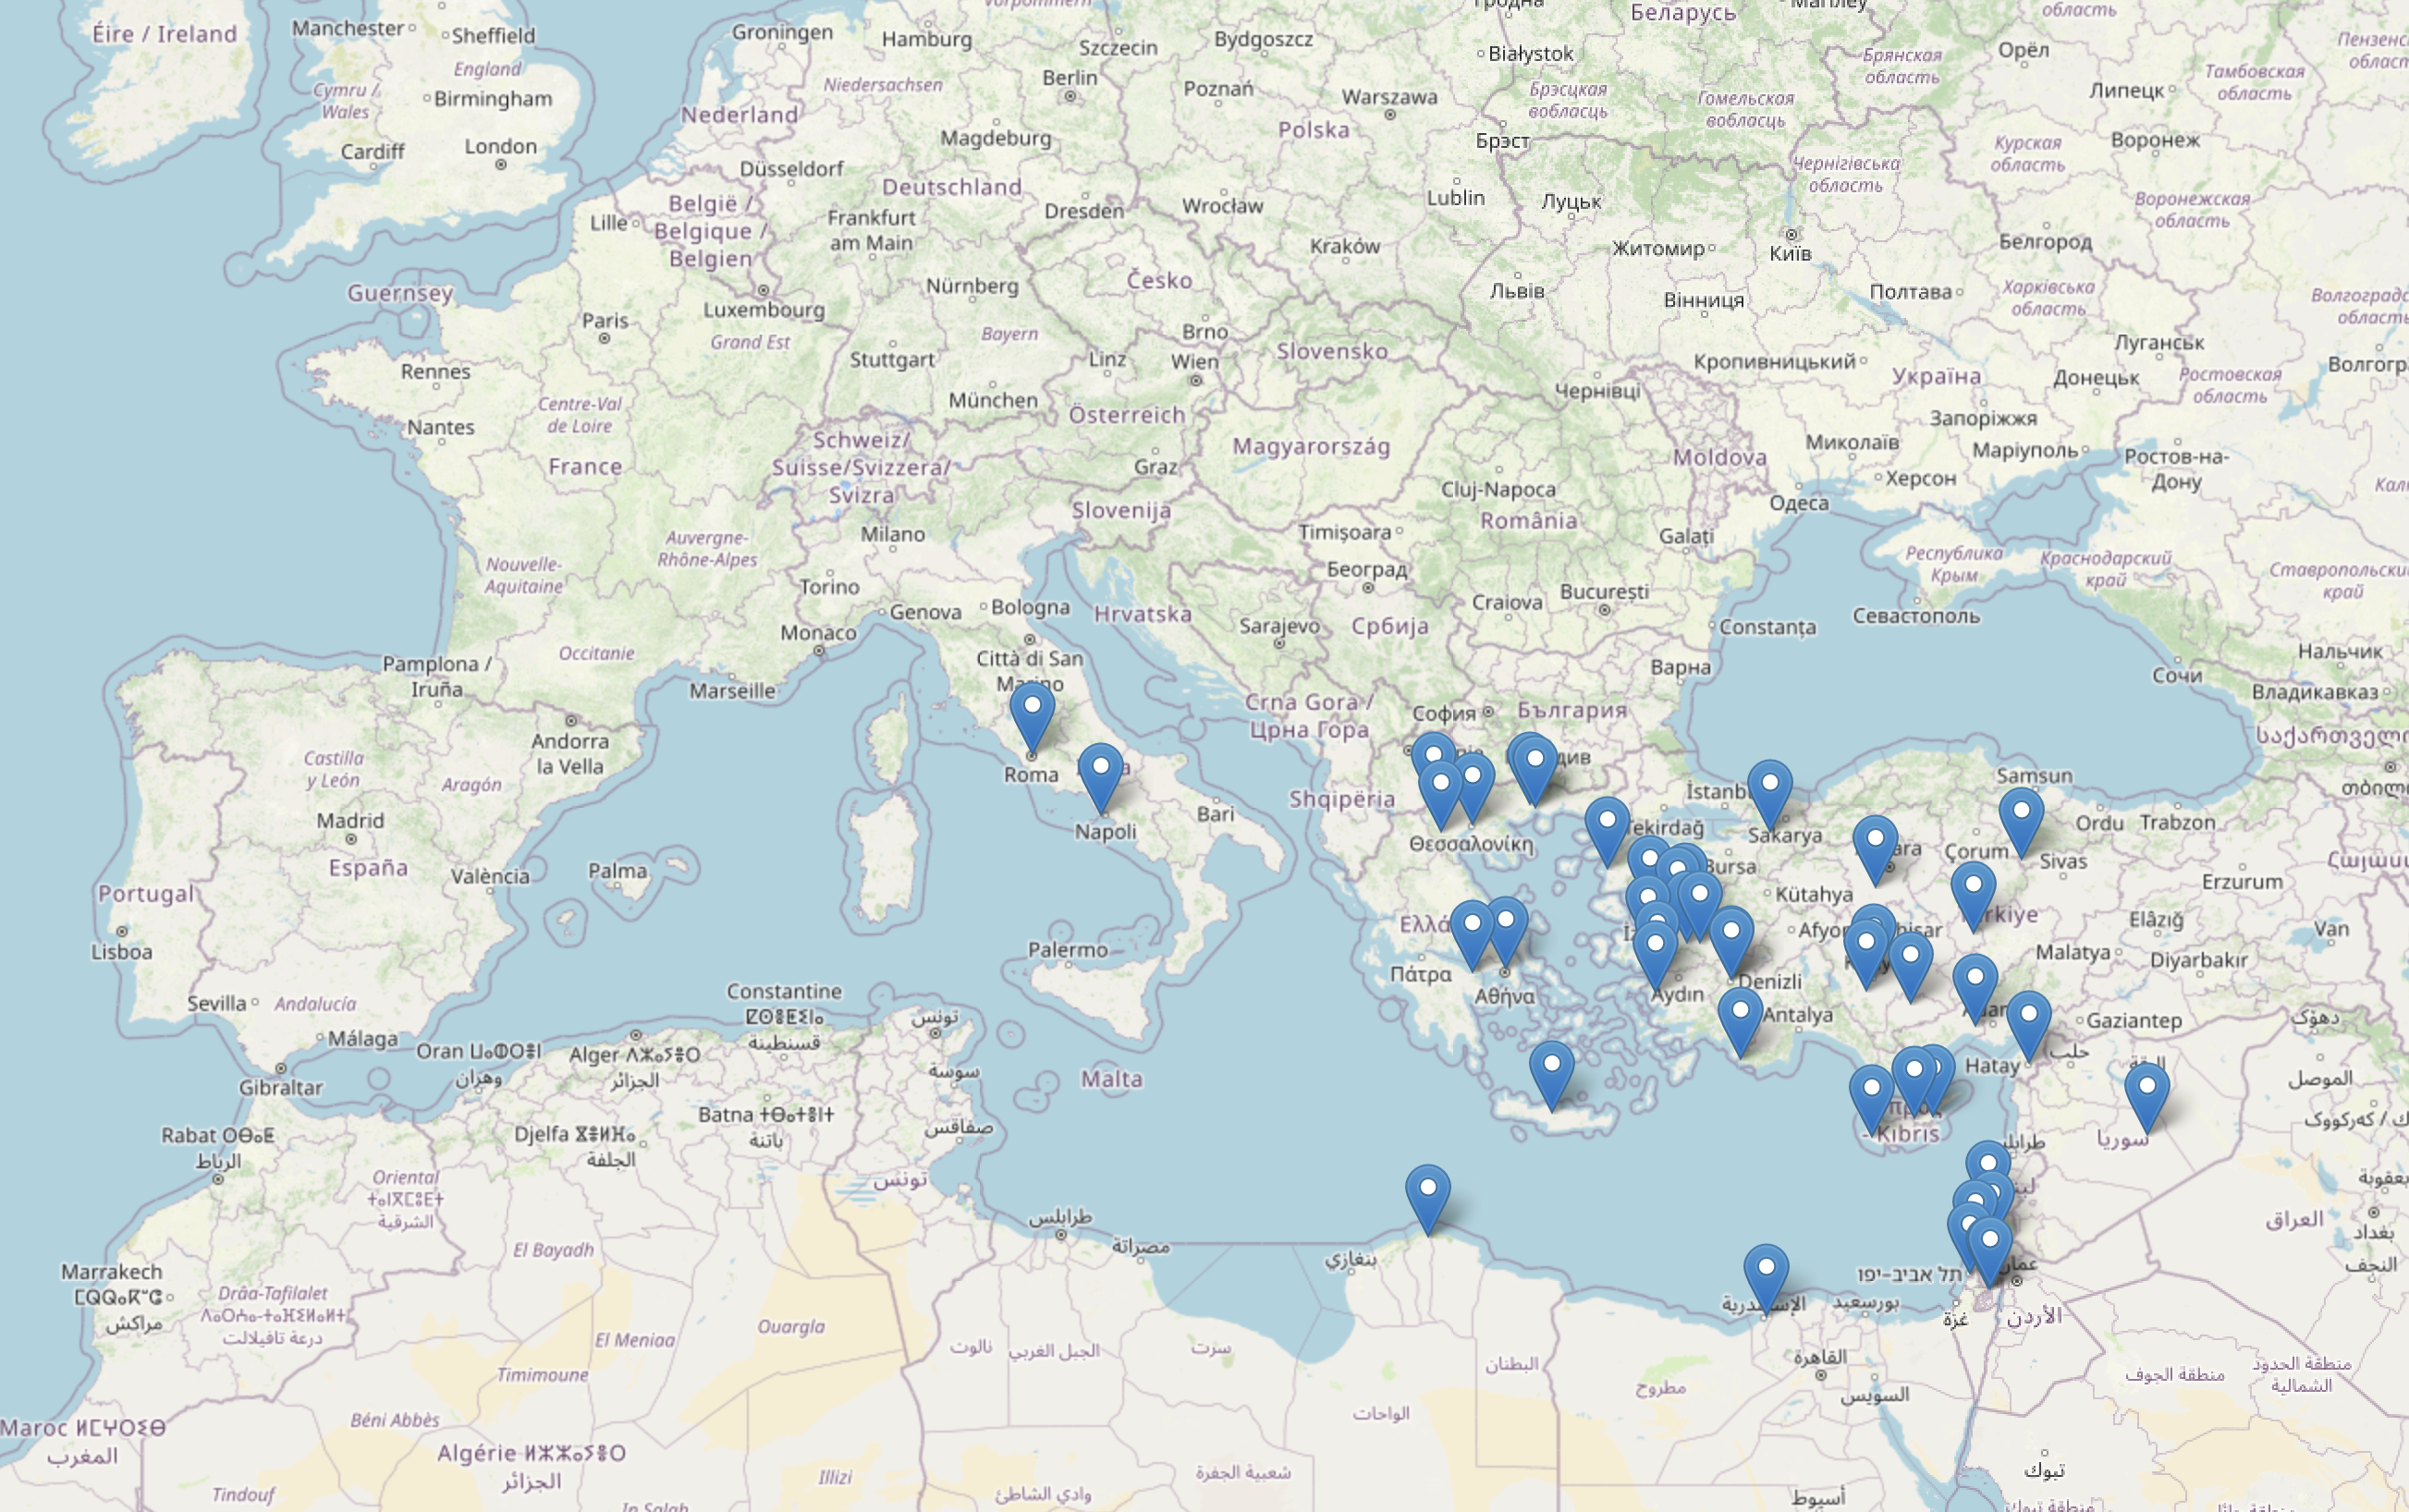
\includegraphics[width=\textwidth, keepaspectratio]{locations_map}
    \caption{Map of all the locations mentioned in the Acts and the epistles.}
    \label{fig:figure}
\end{figure}

For those geographically inclined you can spot the near perfect correlation with the borders of Eastern Roman Empire.
Of note is the trip to Rome, which was substantially different in nature to the other trips.
\href{https://en.wikipedia.org/wiki/Byzantine_Empire_under_the_Theodosian_dynasty\#/media/File:4KTHEODOSIAN.png}{Rome Map}

\paragraph{3.
The striking statistics of the cities mentioned in the Acts and the epistles are that they are all in the former Greek empire, and not one mention of a city in the Roman empire that was not part of the former Greek empire.}\label{par:the-striking-statistics-of-the-cities-mentioned-in-the-acts-and-the-epistles-are-that-they-are-all-in-the-former-greek-empire-and-not-one-mention-of-a-city-in-the-roman-empire-that-was-not-part-of-the-former-greek-empire.}

This fact makes any theory that deems Christianity as a religious and not a political movement immediately highly implausible.

\paragraph{4.
Finally we consider the apparent minimal resistance to the acceptance of the new religion.}\label{par:finally-we-consider-the-apparent-minimal-resistance-to-the-acceptance-of-the-new-religion.}

The new religion was accepted by the masses in the former Greek empire, and not a single mention of any resistance to the new religion from the Greeks themselves.
The only real opposition comes from the Temple authorities in Jerusalem.
This is consistent with Christianity being a continuation of Greek imperial philosophy, which the Hellenized population already accepted.

\paragraph{5.
We should also consider that even though the religion was so successful at converting the masses, it still had all the conspiratorial parts to it.}\label{par:we-should-also-consider-that-even-though-the-religion-was-so-successful-at-converting-the-masses-it-still-had-all-the-conspiratorial-parts-to-it.}

Early Christians used secret symbols to identify each other, they frequently met in secret, often at night in the catacombs.
This is not unlike the initiation practices of other imperial soldier cults such as Mithras.
The Pauline language of ``soldiers of Christ'' fits this conspiratorial military model.

\paragraph{6.
Consider why the religion was seemingly much more prosecuted than any other religion in the Roman empire.}\label{par:consider-why-the-religion-was-seemingly-much-more-prosecuted-than-any-other-religion-in-the-roman-empire.}

The Roman empire was very tolerant of other religions, and the only time they would prosecute a religion was if it was a threat to the empire.
Christians were persecuted not for worshipping a strange god, but for refusing the Roman emperor cult while insisting that only their Christ was king.
This was a political treason, not theological quibbling.

\paragraph{7.
The phrase ``soldiers of Christ'' is not used explicitly in the Gospels, but it appears prominently in the Pauline Epistles.}\label{par:the-phrase-soldiers-of-christ-is-not-used-explicitly-in-the-gospels-but-it-appears-prominently-in-the-pauline-epistles-particularly-in-the-context-of-the-christian-life-being-compared-to-a-military-struggle-or-a-spiritual-battle.}

The metaphor emphasizes loyalty, discipline, and readiness for conflict under a divine king.
It reflects the military cultic environment of the empire, not a rural Jewish sect.

\paragraph{8.
Paul barely mentions the life of Jesus, and almost never quotes him.}\label{par:paul-barely-mentions-the-life-of-jesus-and-almost-never-quotes-him.}

It is frequently claimed that Paul's religion is not the religion of Jesus, but the religion about Jesus.
There is a shocking lack of references to any of the teachings of Jesus, the Jewish law, and any of the events surrounding Jesus's life and death.
So we may go one step further.
It is a religion focusing on restoring the kingdom of God by resurrecting the office of the Christos, the rightful king of the kingdom of God.
And so to Paul and all the early Christians, it was all about resurrecting a Christ, not teachings of the particular Jesus Christ.
The idea that God will once again send a king that will restore the Greek empire, the kingdom of God, headed by Christos, the rightful earthly king of the kingdom of God.

\paragraph{9.
Using this conspiratorial language clearly worked.}\label{par:using-this-conspiratorial-language-clearly-worked}

Rome did not even realize the new religion's goal was to restore the Eastern Empire until it actually happened.

\paragraph{10.
Alexandria was the capital of the Greek Empire and the center of the Hellenistic world and yet there are no missions or letters to Alexandria.}\label{par:alexandria-was-the-capital-of-the-greek-empire-and-the-center-of-the-hellenistic-world-and-yet-there-are-no-missions-or-letters-to-alexandria.}

The absence of Alexandria in the New Testament is striking, especially considering its significance.
Alexandria was erased from the text, as it was the origin city of Apollos, as well as some of the other companions of Paul such as Mark, Demas, and Luke.
The omission is best explained as deliberate suppression, precisely because Alexandria was already the center of the movement.
Just as the Old Testament largely omits the Ptolemaic empire despite its centrality, so the New Testament minimizes Alexandria while still presuming its leadership.

\subsection{Acts of the Apostles}\label{subsec:acts-of-the-apostles}

Is called the Acts of the Apostles, not acts of the disciples.
Apostles doing imperial work of letting all nations of the empire know the will of the God king.

\paragraph{10.
Acts opens with a royal enthronement}\label{par:acts-opens-with-a-royal-enthronement}

Acts 1:6 --- ``Lord, will you at this time restore the kingdom to Israel?'' This is not a spiritual question.
It implies Jesus had a claim to political kingship.
Your theory: Jesus was understood as the rightful monarch of a revived kingdom---a successor to the Herodian or Hasmonean thrones under Greek imperial ideals.

\paragraph{10.
Jesus is taken up like an emperor}\label{par:jesus-is-taken-up-like-an-emperor}

Acts 1:9--11 --- The Ascension mimics apotheosis scenes (e.g., Alexander, Roman emperors).
It frames Jesus in imperial terms, being enthroned in heaven---like a divine emperor.
This matches your view that Christianity was about loyalty to the ``Christ Emperor.''

\paragraph{10.
The Pentecost scene mimics an imperial inauguration}\label{par:the-pentecost-scene-mimics-an-imperial-inauguration}

Acts 2 --- Multilingual miracle and mass conversion reflects the imperial ideal of uniting nations under one divine king.
The language of ``tongues'' is political: the emperor's message is for all nations.

\paragraph{10.
Acts 5: The trial of the apostles}\label{par:acts-5-the-trial-of-the-apostles}

Gamaliel references past revolutionary figures---Theudas and Judas the Galilean.
This acknowledges that messianic revolts were political, and that Jesus' movement was seen in similar terms.

\paragraph{10.
Stephen's speech in Acts 7 is anti-Temple}\label{par:stephens-speech-in-acts-7-is-anti-temple}

Stephen attacks the Temple and Mosaic tradition, echoing Philo and Stoic-influenced criticisms of Jewish legalism.
This supports the view that early Christianity rejected the Mosaic religion and aligned more with philosophical monotheism.

\paragraph{10.
Paul as imperial envoy}\label{par:paul-as-imperial-envoy}

Paul appeals to Caesar, travels through Greek cities, and preaches to Hellenized elites.
His speeches (e.g., Acts 17 in Athens) are clearly political-philosophical, not sectarian Jewish.
Acts frames Paul as a philosopher-diplomat for the Christ-emperor.

\paragraph{11.
Acts ends without resolution}\label{par:acts-ends-without-resolution}

The book ends in Rome, with Paul freely preaching ``the kingdom of God.''
It lacks a narrative climax because its real message is that the empire is now Christian.
It presumes a pre-existing audience that sees Christianity as a political-theological force.

\subsubsection{James the Just}\label{par:james-the-just}

\paragraph{1.
James the Just also wrote an epistle to all nations.}\label{par:james-the-just-also-wrote-an-epistle-to-all-nations.}

He was the brother of Jesus, and the next in line to the throne.
Much like Jesus Christ the Soter, James also held a royal title, the Just.

James the Just also wrote an epistle to all nations, which is included in the New Testament.
James, like John, refers to the same understanding of Logos as Philo of Alexandria.
The writing style of James and John also bears a striking resemblance to the writing style of Philo of Alexandria.

In Greek, James 1:21 reads as:
``Διὸ ἀποθέμενοι πάσαν ἀκαθαρσίαν καὶ περισσείαν κακίας ἐν πραΰτητι δέξασθε τὸν ἐμφυτον λόγον, ὃς δύναται σῶσαι τὰς ψυχὰς ὑμῶν.''
Transliteration: ``Dio apothemenoi pasan akatharsian kai perisseian kakias en prautēti dexasthē ton emphuton logon, hos dynatai sōsai tas psychas hymōn.''
A literal translation: ``Therefore, putting away all filthiness and the overflow of wickedness, with meekness receive the implanted word, which is able to save your souls.''

It should go without saying that the advanced writing style of James and John is not something that would be expected from a simple fisherman or a son of a carpenter.
Rather, it confirms Alexandrian philosophical schooling at the very center of the Greek imperial world.


\chapter{The Purple Phoenix Raises Again}\label{ch:the-purple-phoenix-raises-again}
\section{Chapter 5 - Purple Phoenix Raises}\label{par:chapter-5---purple-phoenix-raises}

A common unassailable but certainly wrong assumption of modern scholarship is that all early christian literature was written in Greek because Greek was the lingua franca of the Roman empire.

According to this claim we would expect Julius Caesar, the People and the Senate of Rome, Virgil, Seneca to all be fluent and write and speak extensively in Greek.

In fact, it is correct Greek was the administrative language of nearly the oll of the former Greek empire which later became known as the Eastern Roman Empire.

Notably nearly all Christian writers including Clement of Rome, Ignatius of Antioch, Polycarp, Justin Martyr, Irenaeus, Origen wrote in Greek.

The first non-greek church father is Tertulian close to the end of second century.

In this chapter we want to highlight that Christianity was Greek-only religion, while there were many mentions of Jesus in non-greek sources, and very notably, religious sources about written in coptic, were not considered the same religion as Christianity.

In this chapter we look at the writings of the church fathers from the prism of the Byzantine Empire resurgence.

\paragraph{0.
Alexandria Egypt suffered enormous hardship and persecution during the Roman Empire.}\label{par:alexandria-egypt-suffered-enormous-hardship-and-persecution-during-the-roman-empire.}

The 200-year struggle of the Rome to conquer all the Greek world ended in enormous tax burden of the newly conquered territories.
Almost all tax revenue of the Roman Empire at the time of Jesus and shortly after was coming from the newly conquered territories of the Greeks and nearly half of it came from Egypt.
It is often misunderstood that Egypt was simply so wealthy and more developed than the rest of the world that it could account for such a large share of the tax revenue.
Egypt was indeed the richest, but by no means by such a large margin.
The tax was simply so high to transfer the wealth of the Greeks to Rome and destroy the heartland of the Greek world and their capability to resist in the future.
Given the hardships that the Greeks suffered, there should be no doubt they would seek to restore their kingdom of God and not be ruled by the beast of Rome.

Egypt was considered property of the emperor and not subject to normal senatorial and imperial governance system.

\paragraph{1.
Many other early Christian texts were written to seemingly promote the restoration of the Eastern Roman Empire.}\label{par:many-other-early-christian-texts-were-written-to-seemingly-promote-the-restoration-of-the-eastern-roman-empire.}

The Clement of Alexandria, a very prominent early Christian theologian, wrote in his book ``Stromata'' that the true philosophy was the Greek philosophy, and that the Greek philosophy was the true philosophy.
He wrote of the bird Phoenix, which was a symbol of the Eastern Roman Empire, and that the bird was purple, which was the color of the Eastern Roman Empire.
Universally the phoenix has been assumed to be a symbol of the resurrection of Jesus, but the phoenix was a symbol of the Eastern Roman Empire.

\paragraph{2.
The very famous shields of with the Chi-Rho symbol were a symbol of the creation of the Eastern Roman Empire.}\label{par:the-very-famous-shields-of-with-the-chi-rho-symbol-were-a-symbol-of-the-creation-of-the-eastern-roman-empire.}

The creation of the Eastern Roman Empire as a kingdom of God ruled by the Christ by a Christian army of Christian emperor Constantine was a very important event in the history of the world.
At that point the symbol of the soldiers was not a cross.
The symbol of the soldiers was the Chi-Rho symbol, which was a symbol of the Christos.
Note the shields only signified the Christos on them and not Jesus directly, which may have been a designation that we are the soldiers of the Christ, rightful king of the kingdom of God, and the battles for the restoration of the kingdom of the Christos.
If the war was thought for religious reasons primarily, there would have likely been a lot more emphasis on the cross and mass conversions to Christianity, and we do not that being strongly emphasized in the historical records of this particular war.
We do however see the large emphasis on political changes and restoring the rule in the East.

\paragraph{2.
Rome converting to Christianity matched in time with Rome splitting into two empires, the Western Roman Empire and the Eastern Roman Empire.}\label{par:rome-converting-to-christianity-matched-in-time-with-rome-splitting-into-two-empires-the-western-roman-empire-and-the-eastern-roman-empire.}

The restoration of the Eastern Roman Empire was the actual goal of the christians and christians taking over corresponded with the restoration of the Eastern Roman Empire.

\paragraph{3.
Hippolytus of Rome (c.~170--235 AD) and other early Christian thinkers believed that the fall of Rome was part of God's plan for the eventual establishment of Christ's eternal empire.}\label{par:hippolytus-of-rome-c.-170235-ad-and-other-early-christian-thinkers-believed-that-the-fall-of-rome-was-part-of-gods-plan-for-the-eventual-establishment-of-christs-eternal-empire.}

\paragraph{4.
The Apocalyptic Restoration - The End of Time and the Empire:}\label{par:the-apocalyptic-restoration---the-end-of-time-and-the-empire}

In the Apocalyptic literature, particularly found in Revelation, Christians looked forward to a new heaven and new earth (Revelation 21).
The New Jerusalem would come down from heaven, and it was often interpreted as both a spiritual and literal kingdom that would restore what was lost with the fall of the world.
Eschatological visions were tied to the restoration of an empire under Christ's rule, not just in a spiritual sense, but in a political and cosmic sense.
The Roman Empire was viewed by some as a precursor to the final divine kingdom.

\paragraph{5.
Similarly, Origen (c.~185--254 AD) also held that Christianity could restore the world order.
He saw the future reign of Christ as the ultimate restoration of order, justice, and peace in a new universal kingdom, where Christianity would reign.}\label{par:similarly-origen-c.-185254-ad-also-held-that-christianity-could-restore-the-world-order.-he-saw-the-future-reign-of-christ-as-the-ultimate-restoration-of-order-justice-and-peace-in-a-new-universal-kingdom-where-christianity-would-reign.}

\paragraph{6.
Irenaeus (c.~130--202 AD) - In his work Against Heresies, Irenaeus speaks about the role of the Roman Empire in God's providence and the eventual victory of Christianity.
He hints at a future unity and a cosmic victory which could be seen as the ``restoration'' of the world through Christ's reign.}\label{par:irenaeus-c.-130202-ad---in-his-work-against-heresies-irenaeus-speaks-about-the-role-of-the-roman-empire-in-gods-providence-and-the-eventual-victory-of-christianity.-he-hints-at-a-future-unity-and-a-cosmic-victory-which-could-be-seen-as-the-restoration-of-the-world-through-christs-reign.}

Irenaeus of Lyons (c.~130--202 AD) In his Against Heresies, Irenaeus focuses on defending orthodox Christian beliefs, but there are also passages where he highlights the role of the Roman Empire in God's plan.
He stresses that the empire's rule is part of God's providence and suggests that its peaceful reign is a way of preparing the world for Christ's return, offering a sense of the empire's importance in Christian restoration.

\paragraph{7.
Tertullian (c.~155--240 AD) - In his writings, such as Apology and On the Resurrection of the Flesh, Tertullian often implies the eventual triumph of Christianity within the Roman Empire, framing it as part of a divine plan.
While he doesn't directly speak of the ``restoration'' of the empire, there is a sense of Christianity fulfilling the destiny of the Roman state.}\label{par:tertullian-c.-155240-ad---in-his-writings-such-as-apology-and-on-the-resurrection-of-the-flesh-tertullian-often-implies-the-eventual-triumph-of-christianity-within-the-roman-empire-framing-it-as-part-of-a-divine-plan.-while-he-doesnt-directly-speak-of-the-restoration-of-the-empire-there-is-a-sense-of-christianity-fulfilling-the-destiny-of-the-roman-state.}

\paragraph{8.
Eusebius of Caesarea (c.~260--340 AD)}\label{par:eusebius-of-caesarea-c.-260340-ad}

In his work Ecclesiastical History and Life of Constantine, Eusebius explicitly presents the rise of Constantine and the establishment of Christianity as the fulfillment of God's plan for the Roman Empire.
He sees Constantine's reign as a ``restoration'' of the empire, aligning it with divine will.
This reflects the idea that Christianity would not only restore the empire but also bring it to its true, Christian purpose.

\paragraph{9.
Athanasius of Alexandria (c.~296--373 AD)}\label{par:athanasius-of-alexandria-c.-296373-ad}

In his writings, particularly in his defense against Arianism and his theological works, Athanasius talks about the cosmic victory of Christ over evil, which has implications for the empire's restoration.
He often frames the Christian emperor as the rightful ruler under divine guidance, which could be seen as linking the restoration of the empire to Christ's victory.

\paragraph{10.
Victorinus of Pettau (c.~250--303 AD)}\label{par:victorinus-of-pettau-c.-250303-ad}

In his Commentary on the Apocalypse, Victorinus draws connections between the Roman Empire and the eventual triumph of Christianity.
Like many of his contemporaries, he believes that the empire is part of God's plan and that its ultimate transformation into a Christian empire would bring about the fulfillment of prophecy.
This can be seen as a form of ``restoration'' through the christianization of the empire.

\paragraph{11.
The revolt is not militaristic Rome chose to spiritually convert to Christianity, and the Eastern Roman Empire was restored peacefully while the Christian writers started to praise rome.}\label{par:the-revolt-is-not-militaristic-rome-chose-to-spiritually-convert-to-christianity-and-the-eastern-roman-empire-was-restored-peacefully-while-the-christian-writers-started-to-praise-rome.}

Augustine of Hippo (354--430 AD) -- Expanded In City of God, Augustine offers a vision where the fall of the Roman Empire is viewed through a Christian lens.
He argues that the decline of the empire does not indicate the failure of divine providence.
While he focuses on the spiritual aspects of empire, he acknowledges the empire's role in preparing the world for the Christian kingdom, suggesting a ``restoration'' of the Roman Empire as a Christian entity in the future.

\paragraph{12.
The Shepherd of Hermas (c.~100-160 AD)}\label{par:the-shepherd-of-hermas-c.-100-160-ad}

Apocalyptic Elements: This early Christian text, written by Hermas, is a visionary work similar in nature to Revelation.
It contains visions and allegories about the future of the Church and the world.
The Shepherd speaks about the coming of the end times and the restoration of the Church through repentance and faithfulness, much like how Revelation portrays the establishment of the New Jerusalem and God's final victory over evil.
Restoration: Hermas depicts the hope of restoration for the Church and its ultimate triumph, paralleling Revelation's theme of the faithful being vindicated at the end of time.

\paragraph{13.
Clement of Alexandria's Exhortation to the Greeks (c.~190 AD)}\label{par:clement-of-alexandrias-exhortation-to-the-greeks-c.-190-ad}

Apocalyptic Elements: In his writings, Clement combines Christian eschatology with Greek philosophy, advocating for the return of the ``Logos'' and the eventual restoration of humanity to divine harmony.
While not strictly apocalyptic in the sense of a Revelation-style vision, his vision of the future aligns with the idea of cosmic renewal.
Restoration: Clement's apocalyptic themes include the eventual restoration of the world through the Logos, an idea that ties back to the restoration of divine order similar to the eschatological views found in Revelation.

\paragraph{14.
Cyprian of Carthage's The Lapsed (c.~250 AD)}\label{par:cyprian-of-carthages-the-lapsed-c.-250-ad}

Apocalyptic Elements: Cyprian writes about the persecution of Christians and the imminent return of Christ.
His works anticipate the final judgment, the victory of the righteous, and the establishment of a divine kingdom.
Restoration: Like other early Christian apocalyptic writers, Cyprian believed that the Church would be restored and triumph over its persecutors, reflecting the broader apocalyptic hope seen in Revelation.


\end{document}
